\documentclass{beamer}
%
% Choose how your presentation looks.
%
% For more themes, color themes and font themes, see:
% http://deic.uab.es/~iblanes/beamer_gallery/index_by_theme.html
%
\mode<presentation>
{
  \usetheme{Madrid}      % or try Darmstadt, Madrid, Warsaw, ...
  \usecolortheme{beaver} % or try albatross, beaver, crane, ...
  \usefonttheme{default}  % or try serif, structurebold, ...
  \setbeamertemplate{navigation symbols}{}
  \setbeamertemplate{caption}[numbered]
}

%\usepackage{blindtext}
%\usepackage{enumitem}
\usepackage{mathrsfs,amsmath,amssymb,bm,amsthm}
\usepackage[english]{babel}
\usepackage[utf8x]{inputenc}
\usepackage{makecell}
\usepackage{longtable}
\usepackage{rotating}
\usepackage{multirow}
\usepackage{algorithmic}
\usepackage[]{algorithm}
\usepackage{multimedia}
\usepackage[font=small,labelsep=none]{caption}
%\usepackage[dvipsnames]{xcolor}

\newcommand{\bmx}{x}
\newcommand{\Real}{\mathbb{R}}
\newcommand{\eps}{\varepsilon}
\newtheorem{assume}{Assumption}
\newtheorem{remark}{Remark}
\newtheorem{proposition}{Proposition}
\newtheorem{notation}{Notation}

\definecolor{mypink1}{rgb}{0.858, 0.188, 0.478}
\definecolor{mypink2}{RGB}{219, 48, 122}
\definecolor{mypink3}{cmyk}{0, 0.7808, 0.4429, 0.1412}
\definecolor{mygray}{gray}{0.6}

\DeclareMathOperator*{\argmin}{\mathrm{argmin}}
\DeclareMathOperator*{\argmax}{\mathrm{argmax}}

\title[Stick Hill-Climbing Optimization]
{A finite-step convergent derivative-free method for unconstrained
optimization}
\author[Y. Huang, XTU]{Yunqing Huang}

\institute[]{Xiangtan University
\\
\vspace{0.3cm}
joint work with Kai Jiang}

%\date{Dec. 30, 2018}
\date{\today }

\begin{document}

\begin{frame}
  \titlepage
\end{frame}

% Uncomment these lines for an automatically generated outline.
\begin{frame}{Outline}
  \tableofcontents[hideallsubsections]
\end{frame}

\AtBeginSection[]
{
\begin{frame}{Outline}
%    \tableofcontents[sectionstyle=show,subsectionstyle=shaded]
	\tableofcontents[currentsection,hideallsubsections]
\end{frame}
}

\section{Introduction}


%\begin{frame}\frametitle{Examples4}
%    Itemize example: \pause
%    \begin{itemize}
%    \item Hello, world! is simple;  \pause
%     \item \LaTeX{} beamer is easy. \pause
%      \end{itemize}
%      Enumerate example: \pause
%      \begin{enumerate}
%      \item \LaTeX{} beamer is powerful, and \pause
%     \item beautiful. \pause
%     \end{enumerate}
%   \end{frame}

%%%%%%%%%%%%%%%%%%%%%%%%%%%%%%%%%%%%%%%%%%%%%%%%%%%%%%%%%%%%%%%%%%%%
\begin{frame}{Unconstrained Optimization}
\begin{align*}
	 \hspace{0.6cm} \min f(x,\gamma)
\end{align*}
where $x$ may be continue variable or discrete data, $\gamma$ is
a set of parameters.

\begin{itemize}
\item Derivative-based optimization: Taylor's expansion
	\begin{itemize}[]
		\item Steepest Descent Method, CG, Newton,
			Quasi-Newton, Trust-Region, \ldots
	\end{itemize}
\item Derivative-free optimization \\
	\begin{itemize}[]
		\item Function derivative evaluation: \large{\textcolor{blue}{costly, unreliable}
			}
			(one cannot trust derivatives or approximate them by finite differences)
	\end{itemize}
\end{itemize}

\end{frame}
%%%%%%%%%%%%%%%%%%%%%%%%%%%%%%%%%%%%%%%%%%%%%%%%%%%%%%%%%%%%%%%%%%%%

%%%%%%%%%%%%%%%%%%%%%%%%%%%%%%%%%%%%%%%%%%%%%%%%%%%%%%%%%%%%%%%%%%%%
\begin{frame}{Derivative-Free Optimization}
	\begin{itemize}
		\item Direct search methods
			\\
			{\large
			\textcolor{blue}{Predetermined search
			directions + Search step} }
			\begin{itemize}
				\item Directional direct-search methods:
					\begin{itemize}
						\item Hooke-Jeeves algorithm (1961);
						 (Generalized) Pattern-search methods
							(Torczon, 1997, Audet-Dennis, 2003);
						Multidirectional search algorithm: Torczon (1991);
						Probabilistic descent directions
							(Gratton-Royer-Vicente-Zhang, 2015),
						\dots
					\end{itemize}
				\item Simplex algorithm: Nelder-Mead (1965),
					\dots
			\end{itemize}
		\item Model-based algorithms
			\\
			{\large \textcolor{blue}{
				Interpolation model like the trust-region method
				but \textbf{NOT} depend on the derivatives
				}}
			\begin{itemize}
				\item
					{\footnotesize
					DFO (Conn-Scheinberg-Toint,
					1997, 1998), UOBYQA (Powell, 2000), NEWUOA
					(Powell, 2004), NEWUOAs (Zhang, 2012), \dots
					}
			\end{itemize}
		\item Heuristic approaches
			\begin{itemize}
				\item Simulated annealing, Genetic algorithm, \ldots
			\end{itemize}
	\end{itemize}
\end{frame}
%%%%%%%%%%%%%%%%%%%%%%%%%%%%%%%%%%%%%%%%%%%%%%%%%%%%%%%%%%%%%%%%%%%%

%%%%%%%%%%%%%%%%%%%%%%%%%%%%%%%%%%%%%%%%%%%%%%%%%%%%%%%%%%%%%%%%%%%%
\begin{frame}{Derivative-Free Optimization}
\begin{itemize}
	\item Molecular geometry conformation
		(minimizing the potential energy of clusters)
	\item Biomedical image processing
	\item Circuit design (tuning parameters of relatively small
		circuits using accurate simulation)
	\item Dynamic pricing
	\item Growing sophistication of computer hardware and
		mathematical algorithms and software (which opens new
		possibilities for optimization)
	\item \dots
\end{itemize}
\end{frame}
%%%%%%%%%%%%%%%%%%%%%%%%%%%%%%%%%%%%%%%%%%%%%%%%%%%%%%%%%%%%%%%%%%%%

\section{Algorithm Description}

%%%%%%%%%%%%%%%%%%%%%%%%%%%%%%%%%%%%%%%%%%%%%%%%%%%%%%%%%%%%%%%%%%%%
\begin{frame}{Motivation: the behavior of the blind for hill-climbing }
\begin{figure}[!htbp]
	\centering
	  \includegraphics[scale=0.2]{./figures/blindman.png}
\end{figure}
\begin{itemize}
	\item Find a higher place with a stick in a circular motion
	\item No predetermined search directions
\end{itemize}
\end{frame}
%%%%%%%%%%%%%%%%%%%%%%%%%%%%%%%%%%%%%%%%%%%%%%%%%%%%%%%%%%%%%%%%%%%%

%%%%%%%%%%%%%%%%%%%%%%%%%%%%%%%%%%%%%%%%%%%%%%%%%%%%%%%%%%%%%%%%%%%%
\begin{frame}{Search Set}


\begin{itemize}
	\item Not neighborhood, BUT boundary
%        
%        a circle in two dimensions, a spherical surface in higher dimensions
%    \item jump out of the local minimum trap quickly with very little memory
%    \item like using fishing net to filter optimal states
\end{itemize}
\begin{figure}[!htbp]
	\centering
	  \includegraphics[scale=0.4]{./figures/nc.png}
\end{figure}
\end{frame}
%%%%%%%%%%%%%%%%%%%%%%%%%%%%%%%%%%%%%%%%%%%%%%%%%%%%%%%%%%%%%%%%%%%%

%%%%%%%%%%%%%%%%%%%%%%%%%%%%%%%%%%%%%%%%%%%%%%%%%%%%%%%%%%%%%%%%%%%%
\begin{frame}{Suspected minimum point}
	
\begin{definition}[Suspected minimum point]
	For a given function $f(x)$,
	$\tilde{x}$ is a suspected minimum point (SMP) if $f(\tilde
	x)\leq f(x)$ for $\forall x\in \partial U(\tilde{x},\rho)$,
	where $\partial U(\tilde{x},\rho)$ is the boundary of
	a neighborhood $U(\tilde{x}, \rho)$ of $\tilde{x}$.
\end{definition}

\begin{itemize}
	\item When $\tilde{x}$ is a minimizer in the neighborhood of
		$U(\tilde{x}, \rho)$, $\tilde{x}$ is a SMP.
	\item The opposite is not always true.
	\item The distance of the SMP and a minimizer is smaller than $\rho$.
%    \item It can be extended to describe suspected maximum point.
\end{itemize}
\end{frame}
%%%%%%%%%%%%%%%%%%%%%%%%%%%%%%%%%%%%%%%%%%%%%%%%%%%%%%%%%%%%%%%%%%%%

%%%%%%%%%%%%%%%%%%%%%%%%%%%%%%%%%%%%%%%%%%%%%%%%%%%%%%%%%%%%%%%%%%%%
\begin{frame}{\textcolor{blue}{Hi}ll-\textcolor{blue}{C}limbing
	method with a \textcolor{blue}{S}tick
	(\textcolor{blue}{\textbf{HiCS}})}

\begin{itemize}
	\item Consider the unconstrained optimization problem
\end{itemize}
\vspace{-0.3cm}
\begin{columns}[c]
	\column{8cm}
\begin{align*}
	\min_x f(x,\gamma),~~ \mbox{where}~~
f: \mathbb{R}^n \rightarrow \mathbb{R}.
\end{align*}
%where $f: \mathbb{R}^n \rightarrow \mathbb{R}$, $\gamma$ is a set of parameters.
%\vspace{0.1cm}
{\scriptsize
\begin{algorithm}[H]
	\caption{\textcolor{blue}{HiCS}}
	\label{alg:shc}
\begin{algorithmic}[1]
	\STATE \textbf{Initialization:} choose $x_0$ and $\rho$.
	\STATE \textbf{for} $k=0,1,2,\dots$
	\\
	\hspace{0.2cm} Find $\bar{x}=\argmin_{y\in O(x_k,\rho)} f(y)$
			\\
	\hspace{0.2cm} If $f(\bar x)<f(x_k)$, then set $x_{k+1}= \bar{x}$.
		  \\
		   \hspace{0.2cm} Otherwise, a SMP is found, and declare the
		   \\
		   \hspace{0.2cm}
		   iteration successful.
\end{algorithmic}
\end{algorithm}
}
	\column{3.5cm}
\begin{figure}[!htbp]
	\centering
	  \includegraphics[scale=0.45]{./figures/shc.png}
\end{figure}
\end{columns}

\end{frame}
%%%%%%%%%%%%%%%%%%%%%%%%%%%%%%%%%%%%%%%%%%%%%%%%%%%%%%%%%%%%%%%%%%%%

%%%%%%%%%%%%%%%%%%%%%%%%%%%%%%%%%%%%%%%%%%%%%%%%%%%%%%%%%%%%%%%%%%%%
\begin{frame}{Finite-Step Convergence}

\footnotesize{
\begin{theorem}[Finite-step convergence]
	Suppose that objective function $f(x)$ is continuous and the
	search domain $\Omega$ is a compact set.
	If there are not two SMPs $x_*$ and $x^*$ satisfying
	$f(x^*)=f(x_*)=A$ when $|x_*-x^*|=\rho$.
	Then HiCS algorithm converges in finite steps.
\end{theorem}
}
\pause
\begin{proof}
\begin{itemize}
\footnotesize{
	\item The stick hill-climbing method produces $\{x_n,
		f(x_n)\}_{n=0}^{\infty}$.
	\item From the assumption, $f(x)$ is bounded, then
		the decreasing sequence $\{f(x_n)\}$ is convergent.
		Assume that $f(x_n)\rightarrow A$.
	\item Exists a convergent subsequence $\{x_{n_k}\}\subset
		\{x_n\}$, s.t.  $x_{n_k}\rightarrow x^*$. $x^*$ is a
		SMP.
	\item We have a bounded subsequence
		$\{x_{n_{k}-1}\}\subset \{x_n\}$ which satisfies
		$|x_{n_k}-x_{n_{k}-1}|=\rho$. Obviously,
		$f(x_{{n_k}-1})\rightarrow A$.
	\item $\{x_{n_{k}-1}\}$ has a
		convergent subsequence $\{x_{n_{m}}\}$, s.t.
		$x_{n_{m}}\rightarrow x_*$. $x_*$ is also a SMP.
	\item From $\{x_{n_{m}}\}$, we have a subsequence
		$\{x_{n_{m}+1}\}\subset\{ x_{n_k}\}$ satisfying
		$|x_{n_m}-x_{n_{m}+1}|=\rho$, and $x_{{n_m}+1}\rightarrow x^*$.
	\item We have $|x^* - x_*|=\rho$, but $f(x^*)=f(x_*)=A$.
		\pause
		~\textcolor{blue}{Contradiction}
		}
\end{itemize}
\end{proof}

\end{frame}
%%%%%%%%%%%%%%%%%%%%%%%%%%%%%%%%%%%%%%%%%%%%%%%%%%%%%%%%%%%%%%%%%%%%

%%%%%%%%%%%%%%%%%%%%%%%%%%%%%%%%%%%%%%%%%%%%%%%%%%%%%%%%%%%%%%%%%%%%
\begin{frame}{Finite-Step Convergence}

\footnotesize{
\begin{theorem}[Finite-step convergence]
	Suppose that objective function $f(x)$ is continuous and the
	search domain $\Omega$ is a compact set.
	If there are not two SMPs $x_*$ and $x^*$ satisfying
	$f(x^*)=f(x_*)=A$ when $|x_*-x^*|=\rho$.
	Then HiCS algorithm converges in finite steps.
\end{theorem}
}
\begin{figure}[!htbp]
	\centering
	  \includegraphics[scale=0.5]{./figures/HiCSprove.png}
\end{figure}

\end{frame}
%%%%%%%%%%%%%%%%%%%%%%%%%%%%%%%%%%%%%%%%%%%%%%%%%%%%%%%%%%%%%%%%%%%%

%%%%%%%%%%%%%%%%%%%%%%%%%%%%%%%%%%%%%%%%%%%%%%%%%%%%%%%%%%%%%%%%%%%%
\begin{frame}{$O(x_k, \rho)\rightarrow O_h(x_k, \rho)$}

The principles of sampling $O(x_k,\rho)$
\textit{\textcolor{blue}{without} a priori information of objective function}
\begin{itemize}
	\item Symmetry
	\item Uniform distribution
	\item As few points as possible
\end{itemize}

\end{frame}
%%%%%%%%%%%%%%%%%%%%%%%%%%%%%%%%%%%%%%%%%%%%%%%%%%%%%%%%%%%%%%%%%%%%

%%%%%%%%%%%%%%%%%%%%%%%%%%%%%%%%%%%%%%%%%%%%%%%%%%%%%%%%%%%%%%%%%%%%
\begin{frame}{$O(x_k, \rho)\rightarrow O_h(x_k, \rho)$}

	\begin{itemize}
		\item Spherical coordinate frame
		\begin{itemize}
			\item Not uniform distribution
			\item Sampling points: $2m^{n-1}$, $n$ is dimension,
				$m$ is the number of equal division points in
				each direction
		\end{itemize}
	\end{itemize}

	\begin{itemize}
		\item Bisection method
		\begin{itemize}
			\item Symmetry, uniform distribution
			\item Sampling points: $2n$
		\end{itemize}
	\end{itemize}
\begin{figure}[!htbp]
	\centering
	  \includegraphics[scale=0.08]{./figures/2Dbisection.png}
	  \hspace{1cm}
	  \includegraphics[scale=0.08]{./figures/3Dbisection.png}
%    \caption{: 2D Gauss function.}
\label{fig:gauss:2drand}
\end{figure}
\end{frame}
%%%%%%%%%%%%%%%%%%%%%%%%%%%%%%%%%%%%%%%%%%%%%%%%%%%%%%%%%%%%%%%%%%%%


%%%%%%%%%%%%%%%%%%%%%%%%%%%%%%%%%%%%%%%%%%%%%%%%%%%%%%%%%%%%%%%%%%%%
\begin{frame}{$O(x_k, \rho)\rightarrow O_h(x_k, \rho)$: Regular Simplex}

\begin{itemize}
	\footnotesize{
	\item Generate $n$-D regular simplex coordinates
		(\textcolor{blue}{$n+1$ vertices}):
		}
	\begin{enumerate}
		\scriptsize{
		\item For a regular simplex, the distances of its vertices
			$\{a_1,\dots,a_n,a_{n+1}\}$ to its center are equal.
		\item The angle subtended by any two vertices of
			$n$-dimension simplex through its center is
			$\theta=arccos(-1/n)$.  }
	\begin{figure}[!htbp]
		\centering
		  \includegraphics[scale=0.19]{./figures/simplex.png}
		  \caption{: \scriptsize{cited from wiki}}
	\end{figure}
	\end{enumerate}
\end{itemize}
%\pause
%\begin{algorithm}[H]
%    \footnotesize{
%    \caption{Generate $n$-D regular simplex coordinates}
%    \label{alg:shc}
%\begin{algorithmic}[1]
%    \STATE Give an $n\times(n+1)$-order zero matrix $x(1:n,1:n+1)$
%    \FOR {$i=1:1:n$}
%    \STATE $x(i,i)=\sqrt{1-\sum_{k=1}^{i-1} [x(k, i)]^{2}}$
%        \FOR {$j=i+1:1:n+1$}
%        \STATE $x(i,j)
%        =\dfrac{1}{x(i,i)}\Big(-\dfrac{1}{n}-x(1:i-1, i)^T \cdot
%        x(1:i-1, j)\Big)$
%        \ENDFOR
%    \ENDFOR
%\end{algorithmic}
%}
%\end{algorithm}
\end{frame}
%%%%%%%%%%%%%%%%%%%%%%%%%%%%%%%%%%%%%%%%%%%%%%%%%%%%%%%%%%%%%%%%%%%%

%%%%%%%%%%%%%%%%%%%%%%%%%%%%%%%%%%%%%%%%%%%%%%%%%%%%%%%%%%%%%%%%%%%%%
%\begin{frame}{Sampling Search Set $O(x_k, \rho)$}
%
%\begin{itemize}
%    \item We rotate the \textcolor{blue}{regular simplex} to sample $O(x_k, \rho)$.
%    \item The rotation matrices can be obtained through Euler angles.
%    \item 2D case:
%\begin{figure}[!htbp]
%    \centering
%      \includegraphics[scale=0.35]{./figures/sketch.png}
%%    \caption{2D schematic diagram of rotating regular simplex for
%%    sampling the search set $O(\bmx_k, \rho)$.}
%\label{fig:obset:sketch}
%\end{figure}
%    \item 3D case:
%  \movie[externalviewer,label=mymovie,width=1in,height=0.2in,poster]{}{simplex_tot.mp4}
%  \hyperlinkmovie[play]{mymovie}{\textcolor{blue}{3D sampling}}
%    \pause
%    \item Computational complexity: \textcolor{blue}{$m(n+1)$}
%\end{itemize}
%%\begin{itemize}
%%\end{itemize}
%\end{frame}
%%%%%%%%%%%%%%%%%%%%%%%%%%%%%%%%%%%%%%%%%%%%%%%%%%%%%%%%%%%%%%%%%%%%%


%%%%%%%%%%%%%%%%%%%%%%%%%%%%%%%%%%%%%%%%%%%%%%%%%%%%%%%%%%%%%%%%%%%%
\begin{frame}{Refinement Strategy}

\begin{itemize}
	\item Principle: No-repeat, Uniform distribution
		\pause
	\item Strategy: Rotation
		\pause
	\item Simplex: rotation matrices can be obtained through Euler angles
	\begin{enumerate}
			\vspace{0.2cm}
		\item 2D case:
	\begin{figure}[!htbp]
		\centering
		  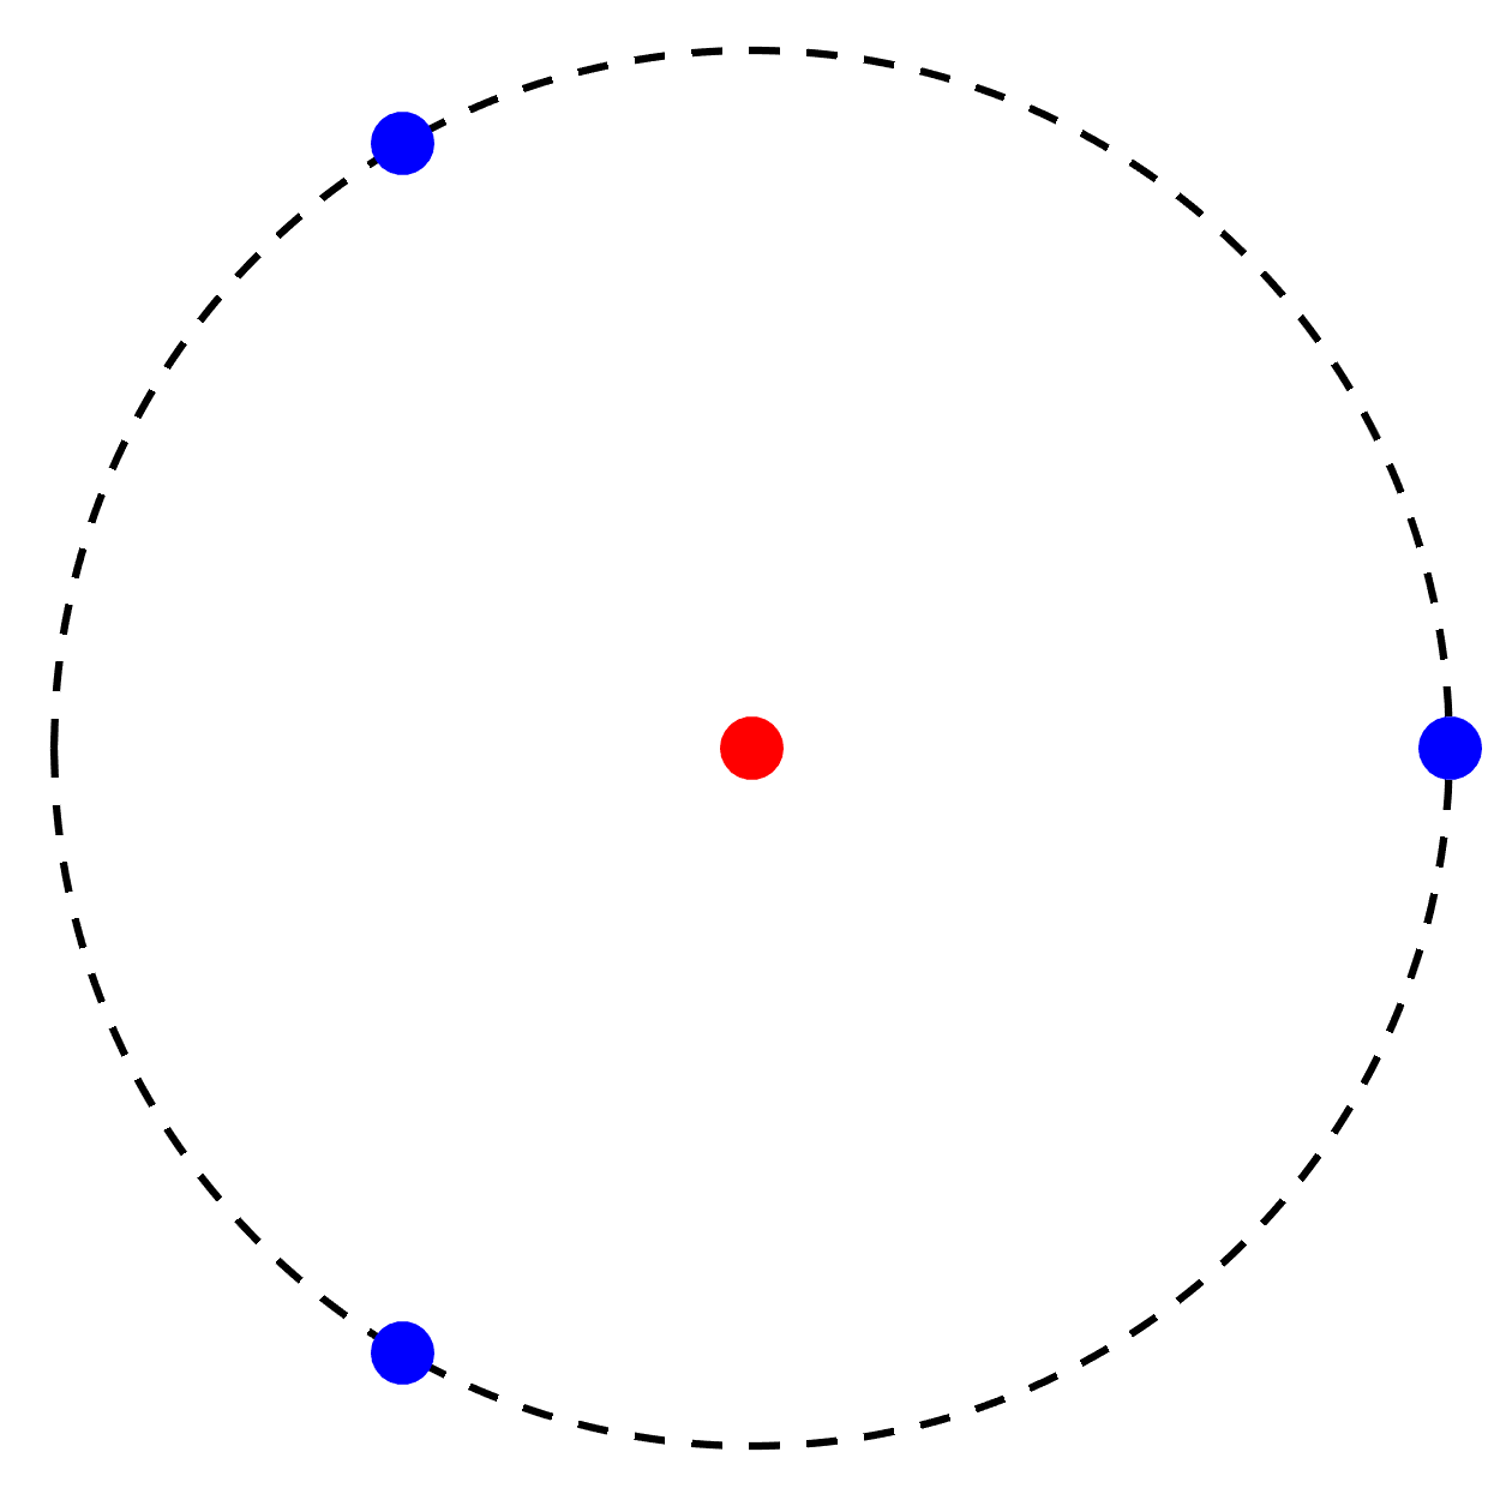
\includegraphics[scale=0.08]{./figures/2D1.png}
		  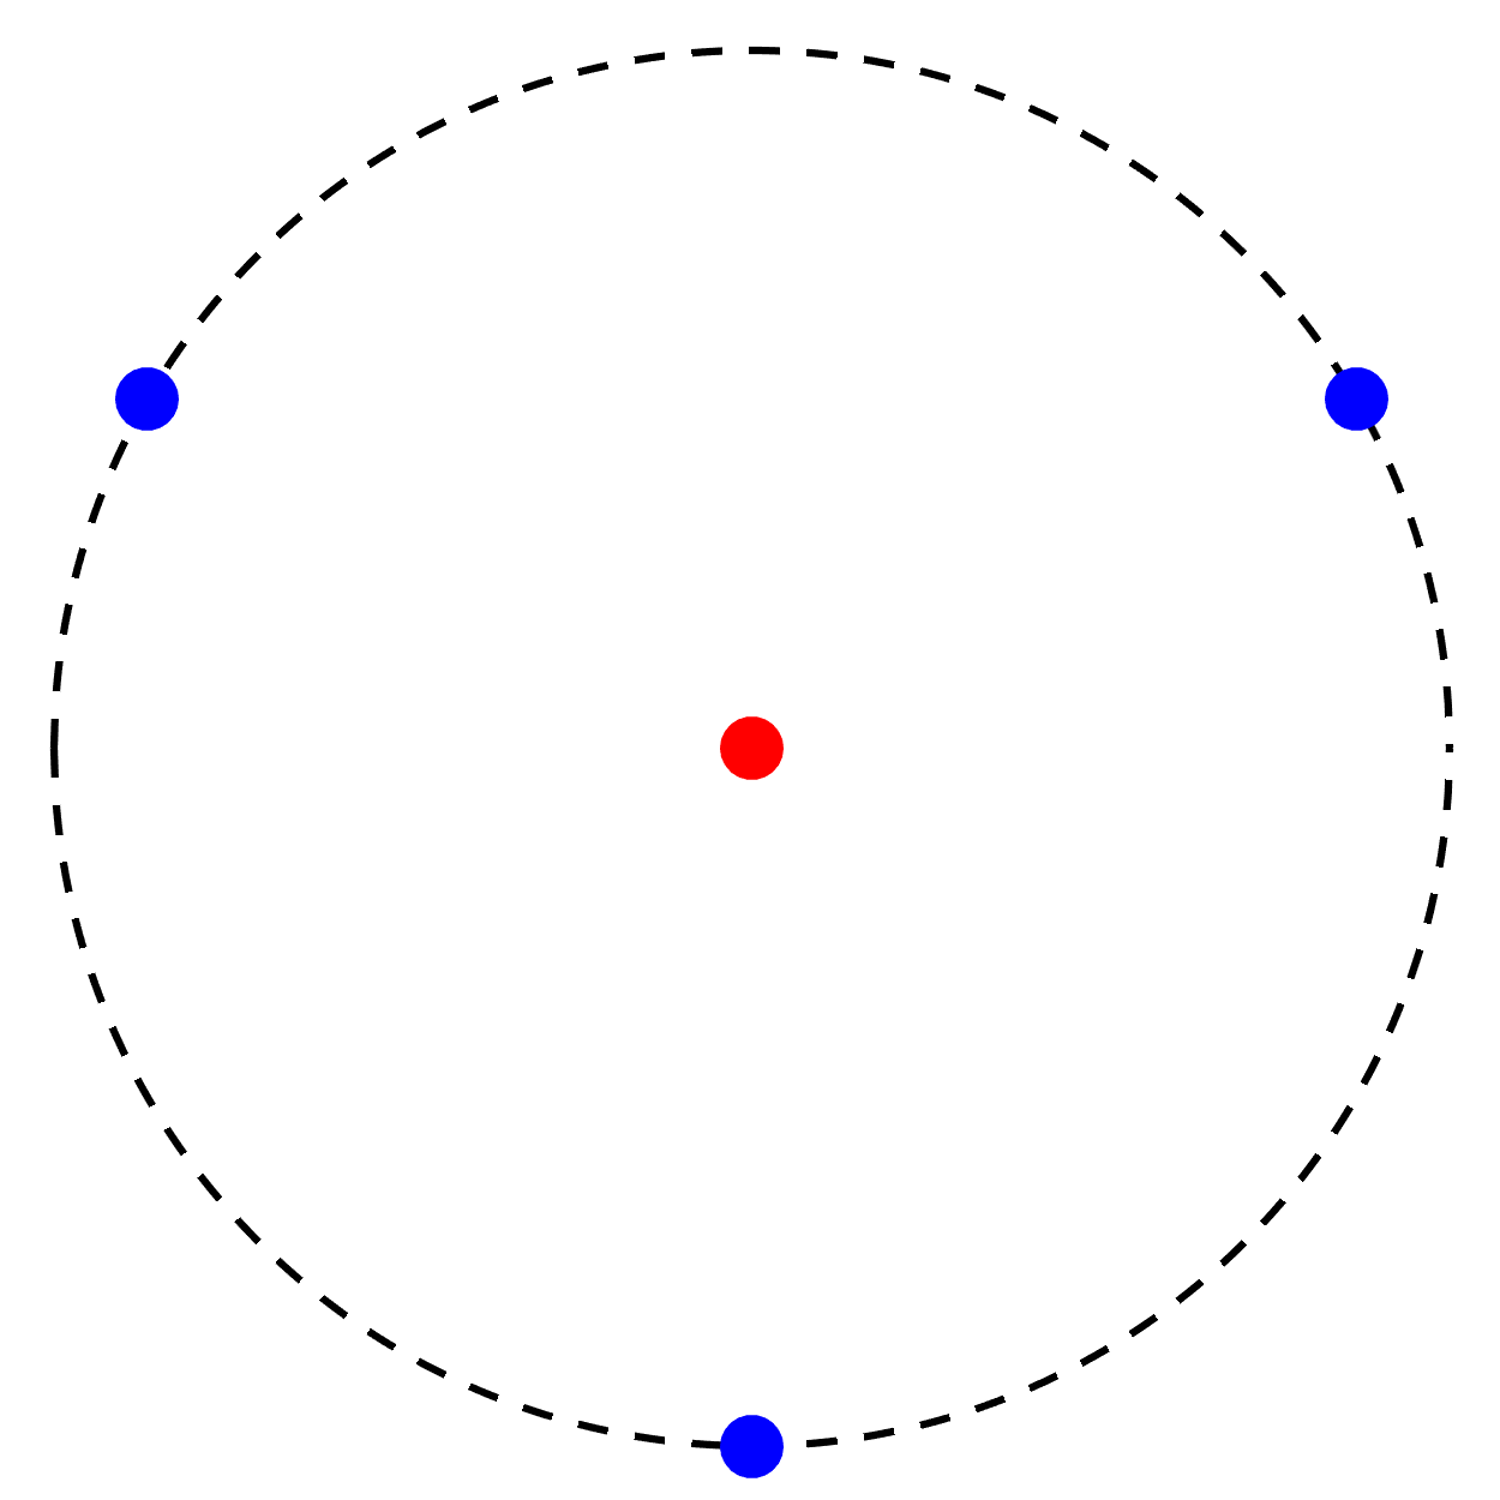
\includegraphics[scale=0.08]{./figures/2D2.png}
		  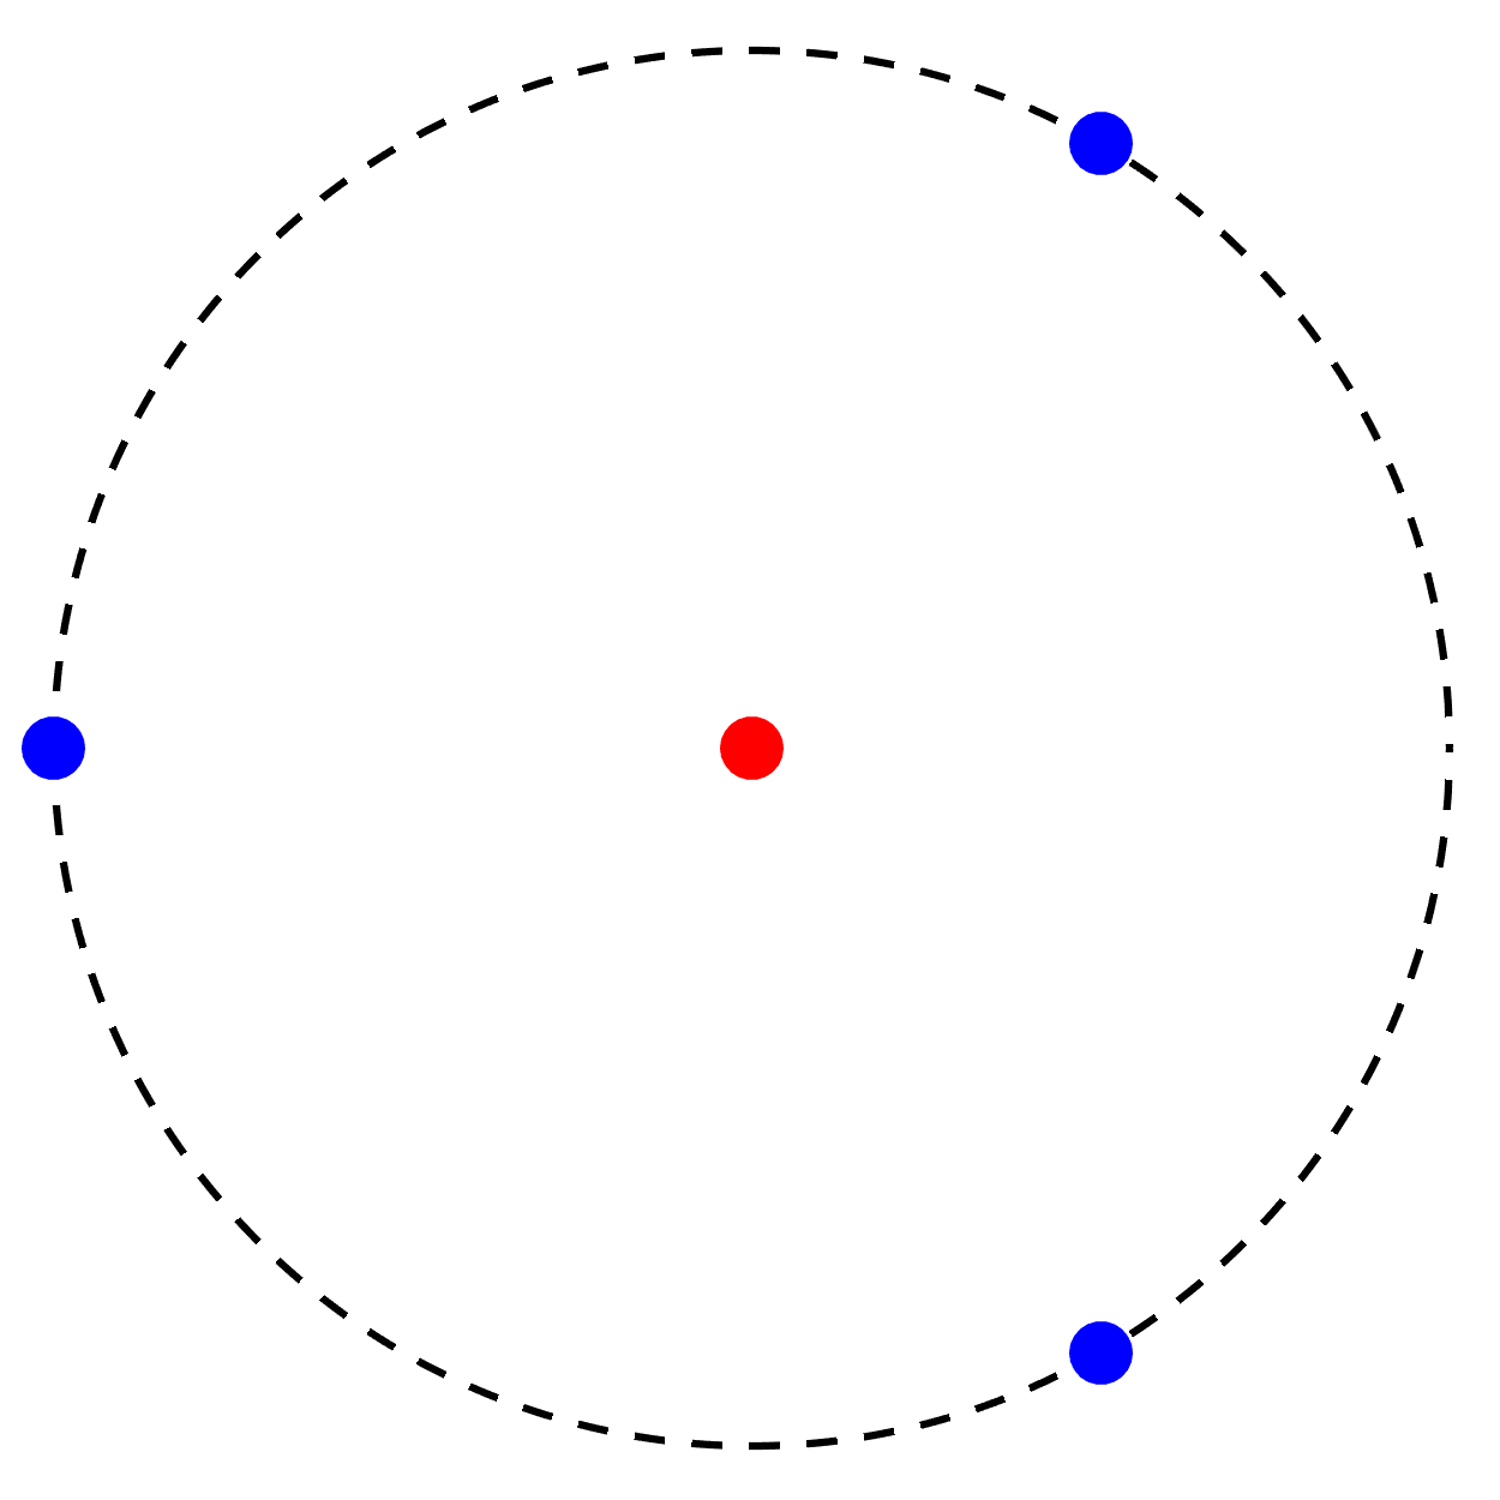
\includegraphics[scale=0.08]{./figures/2D3.png}
		  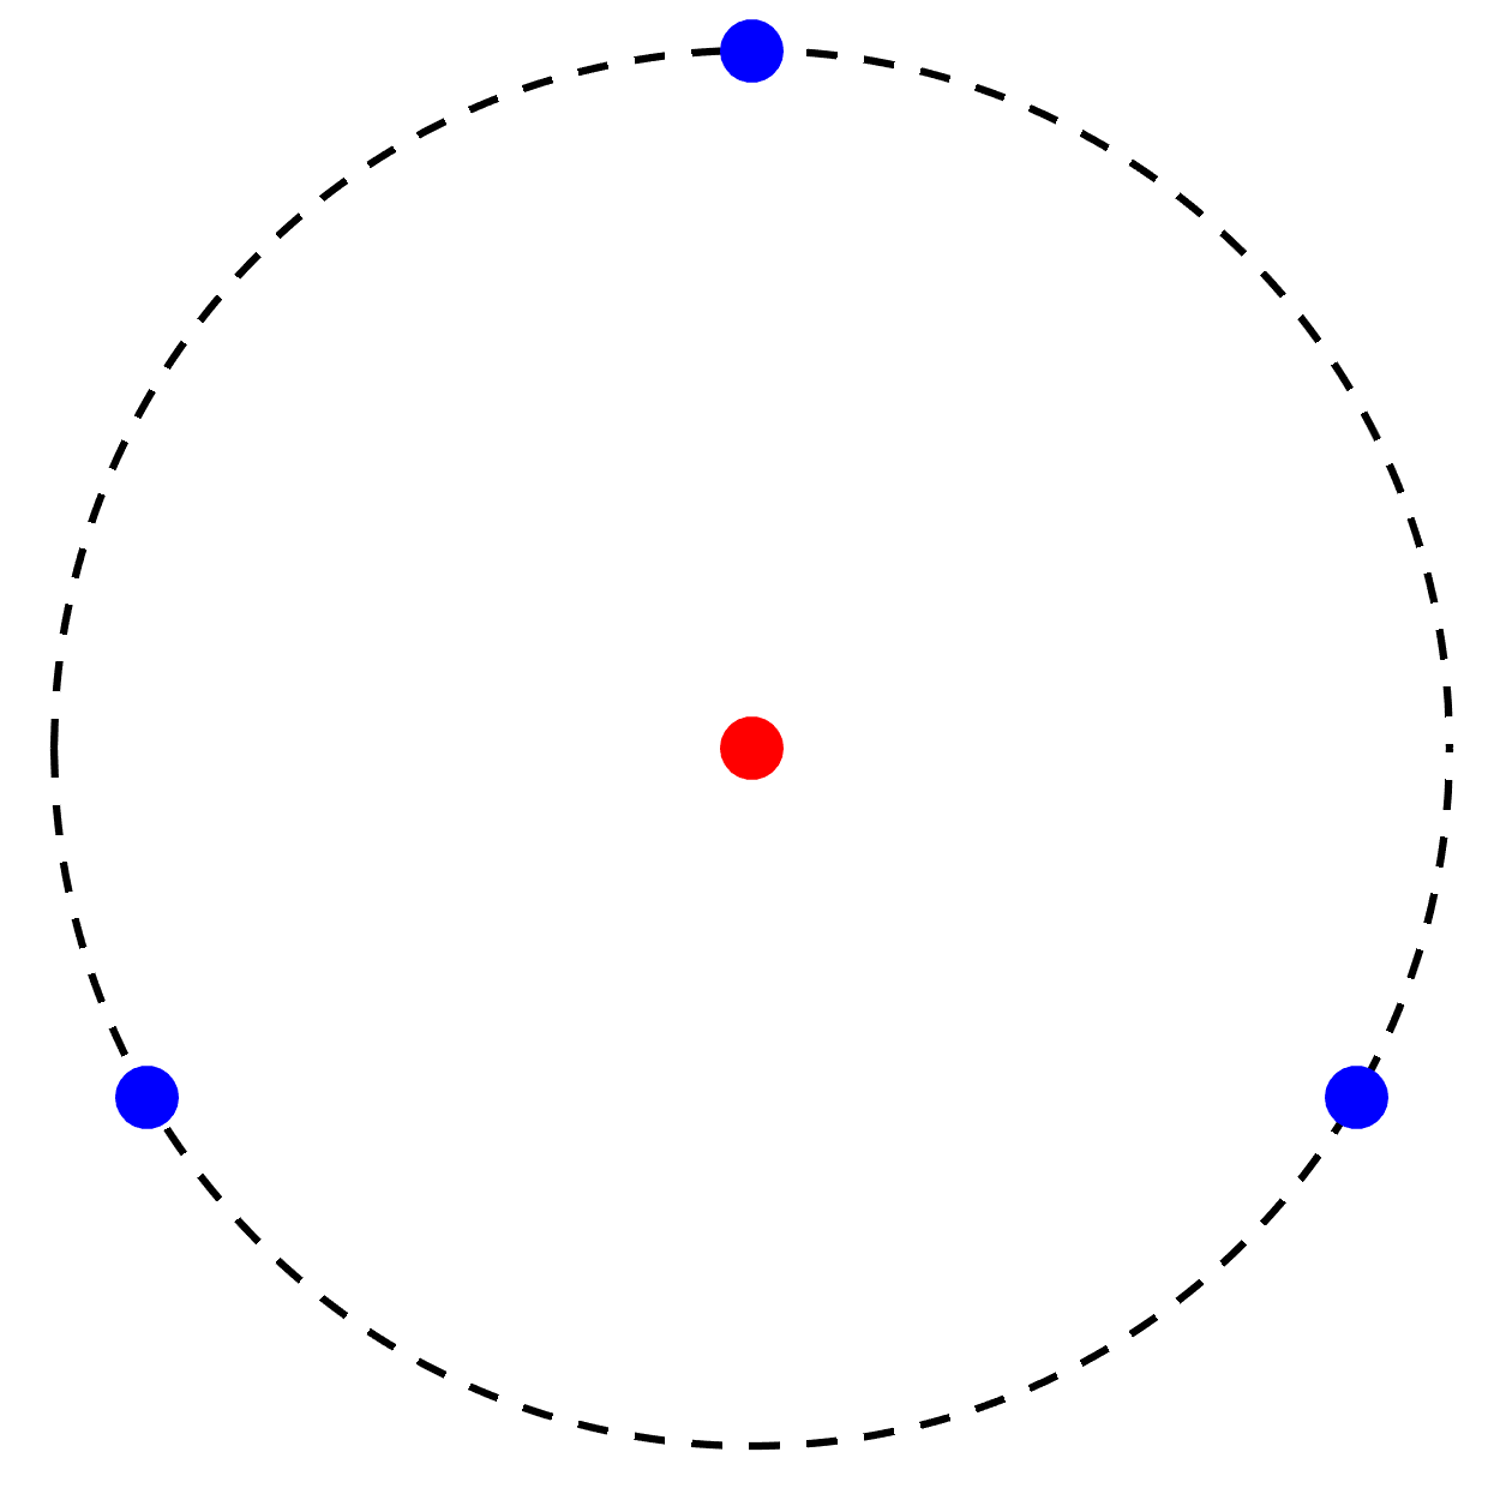
\includegraphics[scale=0.08]{./figures/2D4.png}
%          \includegraphics[scale=0.3]{./figures/sketch.png}
	%    \caption{2D schematic diagram of rotating regular simplex for
	%    sampling the search set $O(\bmx_k, \rho)$.}
	\label{fig:obset:sketch}
	\end{figure}
		\item 3D case:
			\movie[externalviewer,label=mymovie,width=1in,height=0.2in,poster]{}{./figures/3Dschematic.avi}
	  \hyperlinkmovie[play]{mymovie}{\textcolor{blue}{Movie}}
	  \vspace{0.5cm}
	\item Computational complexity: \textcolor{blue}{$m(n+1)$}
	\end{enumerate}
\end{itemize}

\end{frame}


%%%%%%%%%%%%%%%%%%%%%%%%%%%%%%%%%%%%%%%%%%%%%%%%%%%%%%%%%%%%%%%%%%%%
\begin{frame}{HiCS}

\begin{itemize}
	\item In practice, the HiCS algorithm can be given as follows
\end{itemize}

\begin{algorithm}[H]
\footnotesize{
	\caption{HiCS}
\begin{algorithmic}[1]
	\STATE Input $x_0$, $\rho$, and $m_{\max}$
	\FOR {$k=0,1,2,\cdots$}
		\STATE Set $m=0$
		\IF {$m\leq m_{\max}$}
			\STATE Discrete $O(x_k,\rho)$ to obtain $O^m_h(x_k,\rho)$
			\IF {$\exists x_j \in O^m_h(x_k,\rho)$, s.t.  $f(x_j)<f(x_k)$}
				\STATE Set $x_{k+1}=x_j$, and $m=m_{\max}+1$
			\ELSE
				\STATE Set $m = m+1$
			\ENDIF
		\ELSE
			\STATE Declare that find a SMP, end program
		\ENDIF
	\ENDFOR
\end{algorithmic}
}
\end{algorithm}
\end{frame}
%%%%%%%%%%%%%%%%%%%%%%%%%%%%%%%%%%%%%%%%%%%%%%%%%%%%%%%%%%%%%%%%%%%%

%%%%%%%%%%%%%%%%%%%%%%%%%%%%%%%%%%%%%%%%%%%%%%%%%%%%%%%%%%%%%%%%%%%%
\begin{frame}{HiCS: adjust $\rho$ (HiCSa)}

\begin{itemize}
\footnotesize{
	\item We can repeat HiCS algorithm through changing $\rho$
		}
\vspace{-0.2cm}
\begin{algorithm}[H]
\scriptsize{
	\caption{HiCS: adjust $\rho$}
	\label{alg:refined}
\begin{algorithmic}[1]
	\STATE Input $x_0$, $\rho$, $m_{\max}$,
	\textcolor{blue}{$\varepsilon$ and $\eta<1$}
	\IF { \textcolor{blue}{ $\rho>\varepsilon$}}
	\FOR {$k=0,1,2,\cdots$}
		\STATE Set $m=0$
		\IF {$m\leq m_{\max}$}
			\STATE Discrete $O(x_k,\rho)$ to obtain $O^m_h(x_k,\rho)$
			\IF {$\exists x_j \in O^m_h(x_k,\rho)$, s.t.  $f(x_j)<f(x_k)$}
			\STATE Set $x_{k+1}=x_j$, 
				and \textcolor{blue}{$m=m_{\max}+1$} 
%                (Jump out of IF statement) 
			\ELSE
				\STATE Set $m = m+1$
			\ENDIF
		\ELSE
			\STATE \textcolor{blue}{ Set $\rho=\eta\rho$}
		\ENDIF
		\STATE \textcolor{blue}{Set $k=k+1$}
	\ENDFOR
\ENDIF
\end{algorithmic}
}
\end{algorithm}
\pause
\vspace{-0.3cm}
\footnotesize{
	\item The restart mechanism can be obtained by set $\eta>1$
		}
\end{itemize}
\end{frame}
%%%%%%%%%%%%%%%%%%%%%%%%%%%%%%%%%%%%%%%%%%%%%%%%%%%%%%%%%%%%%%%%%%%%

%%%%%%%%%%%%%%%%%%%%%%%%%%%%%%%%%%%%%%%%%%%%%%%%%%%%%%%%%%%%%%%%%%%%%
%\begin{frame}{Adaptive Stick Hill-Climbing (HiCSa) Algorithm}
%
%\footnotesize{
%\begin{itemize}
%    \item The convergent result provide a good initial value to other
%        optimization methods.
%    \item We can further exploit the potential of HiCS algorithm
%        to improve the approximation precision by tuning the search radius $\rho$.
%\end{itemize}
%}
%
%\begin{algorithm}[H]
%\footnotesize{
%    \caption{Adaptive Stick Hill-Climbing Algorithm}
%    \label{alg:pshc}
%\begin{algorithmic}[]
%    \STATE \textbf{Initialization:} Choose $\bmx_0$, $\rho$,
%    and control factor $\eta$.
%    \STATE \textbf{For} $k=0,1,2,\dots$
%    \STATE \hspace{0.5cm} Use \textbf{Algorithm\,\ref{alg:shc}} to find
%    $\bar{\bmx}\in O(\bmx_k, \rho)$ such that
%    $f(\bar\bmx)<f(\bmx_k)$.
%         \\
%         \hspace{0.5cm} If such a point is found, then set
%                         $\bmx_{k+1}= \bar\bmx$.
%          \\
%           \hspace{0.5cm} Otherwise, change the search radius
%          $\rho = \eta \cdot \rho$.
%\end{algorithmic}
%}
%\end{algorithm}
%\end{frame}
%%%%%%%%%%%%%%%%%%%%%%%%%%%%%%%%%%%%%%%%%%%%%%%%%%%%%%%%%%%%%%%%%%%%%


\section{Numerical Results}

\subsection{Gauss Function}

%%%%%%%%%%%%%%%%%%%%%%%%%%%%%%%%%%%%%%%%%%%%%%%%%%%%%%%%%%%%%%%%%%%%%
%\begin{frame}{Gauss Function}
%\footnotesize{
%\begin{align*}
%    f(\bmx) = -h \exp\left( -\sum_{i=1}^n x_i^2/s_i \right),
%    ~~ h =20, s_i = 1.0, i=1,\cdots,n.
%\end{align*}
%\begin{itemize}
%    \item A unique global minimum $\vec{0}$ with $f(\vec{0})=-20$.
%\end{itemize}
%%\begin{figure}[!htbp]
%%    \centering
%%      \includegraphics[scale=0.17]{./figures/gauss.png}
%%    \caption{: 2D Gauss function.}
%%\label{fig:gauss:2drand}
%%\end{figure}
%}
%\end{frame}
%%%%%%%%%%%%%%%%%%%%%%%%%%%%%%%%%%%%%%%%%%%%%%%%%%%%%%%%%%%%%%%%%%%%%

%%%%%%%%%%%%%%%%%%%%%%%%%%%%%%%%%%%%%%%%%%%%%%%%%%%%%%%%%%%%%%%%%%%%
\begin{frame}{Gauss Function}
\footnotesize{
\begin{align*}
	f(\bmx) = -20 \exp\left( -\sum_{i=1}^n x_i^2 \right),
	~~ ~~i=1,\cdots,n.
\end{align*}
\begin{itemize}
	\item A unique global minimum $0$ with $f(0)=-20$.
\end{itemize}
}
\pause
\footnotesize{
	\begin{itemize}
		\item Apply HiCS to 2D Gauss function with $x_0 = (0.57, -0.6)$,
			$\rho=0.3$, $m_{max}=4$.
\end{itemize}
}
\vspace{-0.2cm}
\begin{table}[!htbp]
%\footnotesize{
%\caption{: Iteration information of HiCS}
%}
\begin{center}
\footnotesize{
\begin{tabular}{|c|c|c|}
 \hline
    Iter. & $\ell^2$-distance &  Fun. Val.
 \\\hline
  1 & 8.27587e-01 & -1.00828e+01
 \\ \hline                                                                                                                                       
  1 & 5.40491e-01 & -1.49334e+01
  \\ \hline  
  1 & 2.81712e-01 & -1.84741e+01  
    \\ \hline  
  1 & 2.15853e-01 & -1.90895e+01  
    \\ \hline  
  4 & 8.58004e-02 & -1.98533e+01  
 \\\hline
\end{tabular}
}
\end{center}
\end{table}
\vspace{-0.3cm}
\pause
\footnotesize{
	\begin{itemize}
		\item We can further apply HiCSa approach ($\eta=0.5$) to this case.
	\end{itemize}
\vspace{-0.1cm}
  \movie[externalviewer,label=mymovie,width=1in,height=0.005in,poster]{}{./figures/gauss.avi}
	\hyperlinkmovie[play]{mymovie}{\textcolor{blue}{Movie: Iteration procedure}}
}
\end{frame}
%%%%%%%%%%%%%%%%%%%%%%%%%%%%%%%%%%%%%%%%%%%%%%%%%%%%%%%%%%%%%%%%%%%%

%%%%%%%%%%%%%%%%%%%%%%%%%%%%%%%%%%%%%%%%%%%%%%%%%%%%%%%%%%%%%%%%%%%%
\begin{frame}{10D Gauss Function: finite-step convergence}
\footnotesize{
	\begin{itemize}
		\item HiCS can capture the global minimizer within finite-step iterations
		\item{The iterations of convergence of the HiCS with
			constant \textcolor{blue}{$\rho=0.3$} for
			\textcolor{blue}{10D} Gauss function. The initial
			values were randomly generated in $[-1,1]^2$.}
	\end{itemize}
	}
	\vspace{-0.6cm}
\begin{figure}[!htbp]
	\centering
	  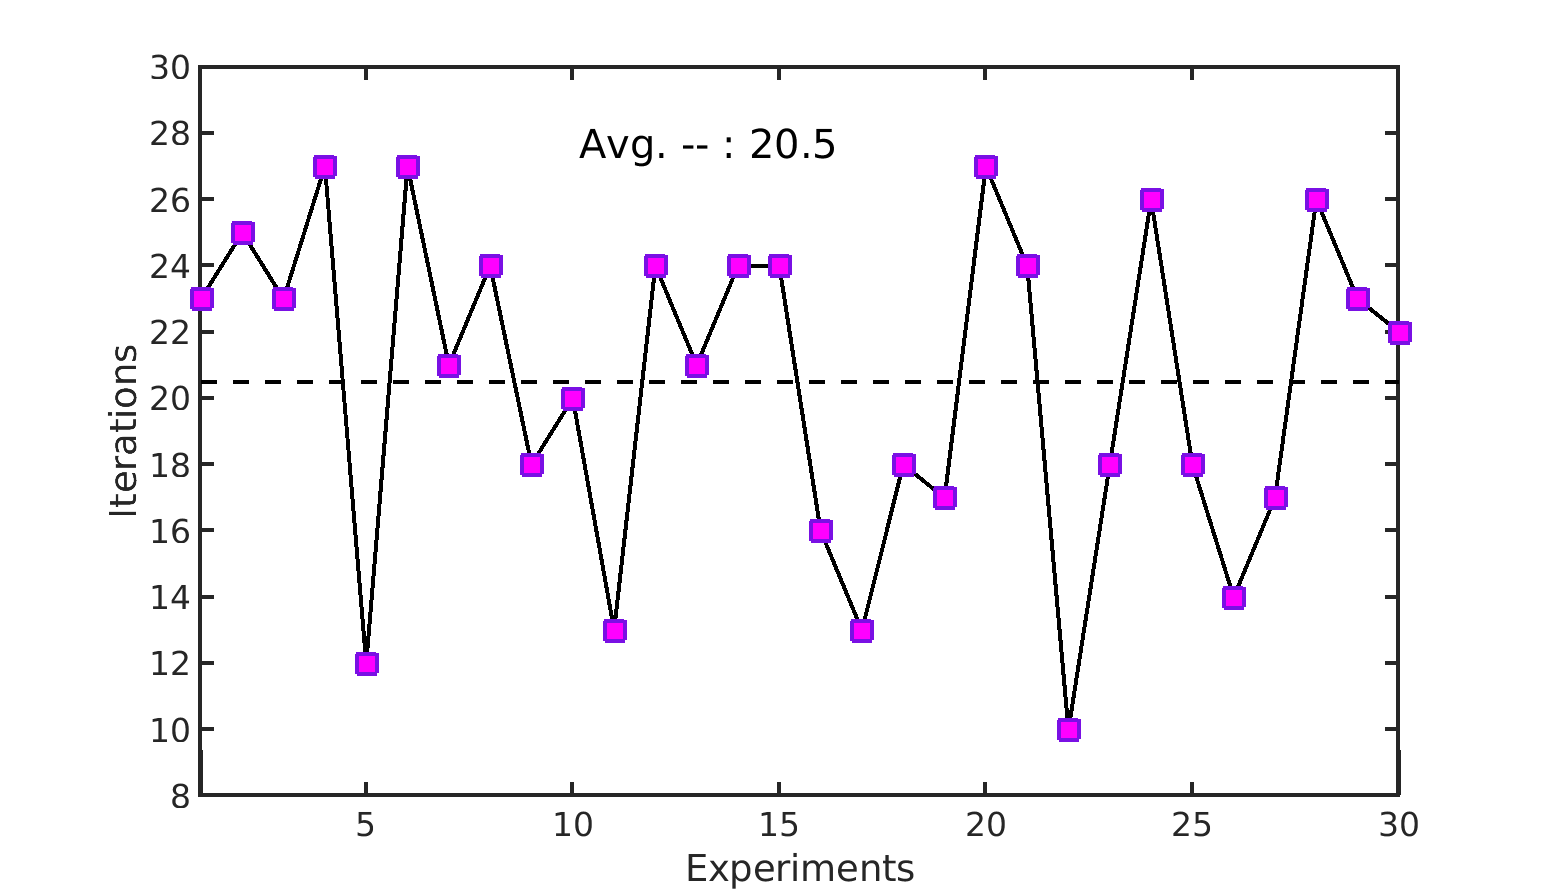
\includegraphics[scale=0.22]{./figures/gauss10Drandr0_3.png}
\end{figure}
\end{frame}
%%%%%%%%%%%%%%%%%%%%%%%%%%%%%%%%%%%%%%%%%%%%%%%%%%%%%%%%%%%%%%%%%%%%

%%%%%%%%%%%%%%%%%%%%%%%%%%%%%%%%%%%%%%%%%%%%%%%%%%%%%%%%%%%%%%%%%%%%
\begin{frame}{10D Gauss Function: finite-step convergence}
\footnotesize{
	\begin{itemize}
		\item{Decreasing \textcolor{blue}{$\rho$} to
			\textcolor{blue}{$0.1$} for 10D Gauss function. The
			initial values were randomly generated in
			$[-1,1]^2$.}
	\end{itemize}
	}
	\vspace{-0.6cm}
\begin{figure}[!htbp]
	\centering
	  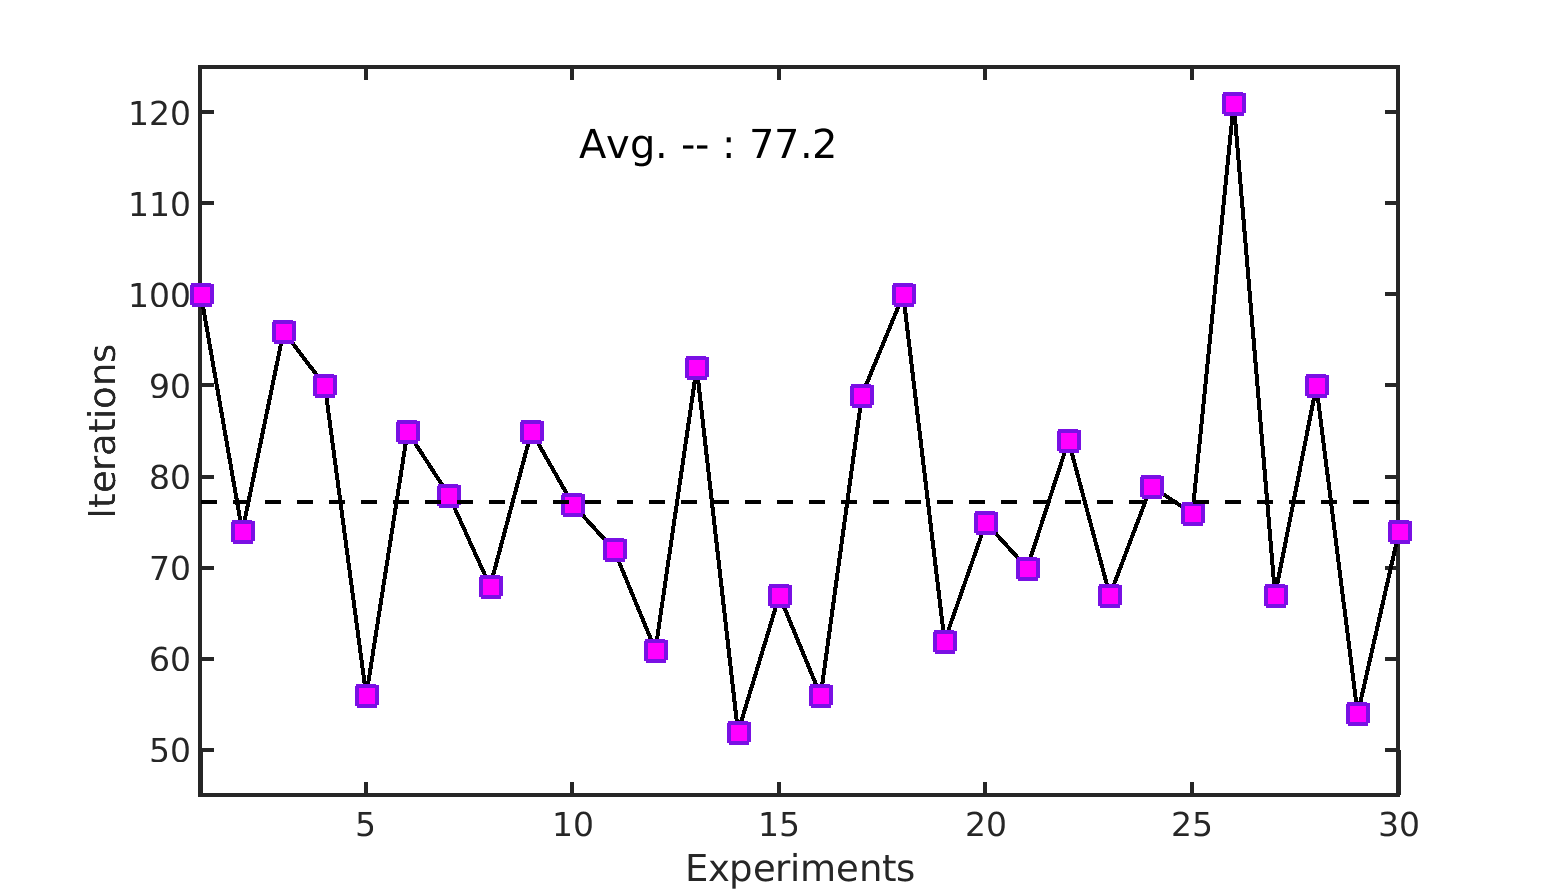
\includegraphics[scale=0.22]{./figures/gauss10Drandr0_1.png}
\end{figure}
\end{frame}
%%%%%%%%%%%%%%%%%%%%%%%%%%%%%%%%%%%%%%%%%%%%%%%%%%%%%%%%%%%%%%%%%%%%

%%%%%%%%%%%%%%%%%%%%%%%%%%%%%%%%%%%%%%%%%%%%%%%%%%%%%%%%%%%%%%%%%%%%%
%\begin{frame}{15D Gauss Function: finite-step convergence}
%\normalsize{
%    \begin{itemize}
%        \item HiCS can capture the global minimizer within finite-step iterations
%    \end{itemize}
%    }
%\begin{figure}[!htbp]
%    \centering
%      \includegraphics[scale=0.22]{./figures/gauss15Drand.png}
%\footnotesize{
%    \caption{: The iterations of convergence of the HiCS with
%    constant $\rho=0.3$ for \textcolor{blue}{15D} Gauss function. The initial
%    values were randomly generated in $[-1,1]^2$.}
%    }
%\end{figure}
%\end{frame}
%%%%%%%%%%%%%%%%%%%%%%%%%%%%%%%%%%%%%%%%%%%%%%%%%%%%%%%%%%%%%%%%%%%%%
%
%%%%%%%%%%%%%%%%%%%%%%%%%%%%%%%%%%%%%%%%%%%%%%%%%%%%%%%%%%%%%%%%%%%%
\begin{frame}{1000D Gauss Function: HiCSa}
\normalsize{
	\begin{itemize}
		\item HiCSa can approximate the minimizer through shrinking $\rho$ 
	\end{itemize}
	}
\begin{figure}[!htbp]
	\centering
	  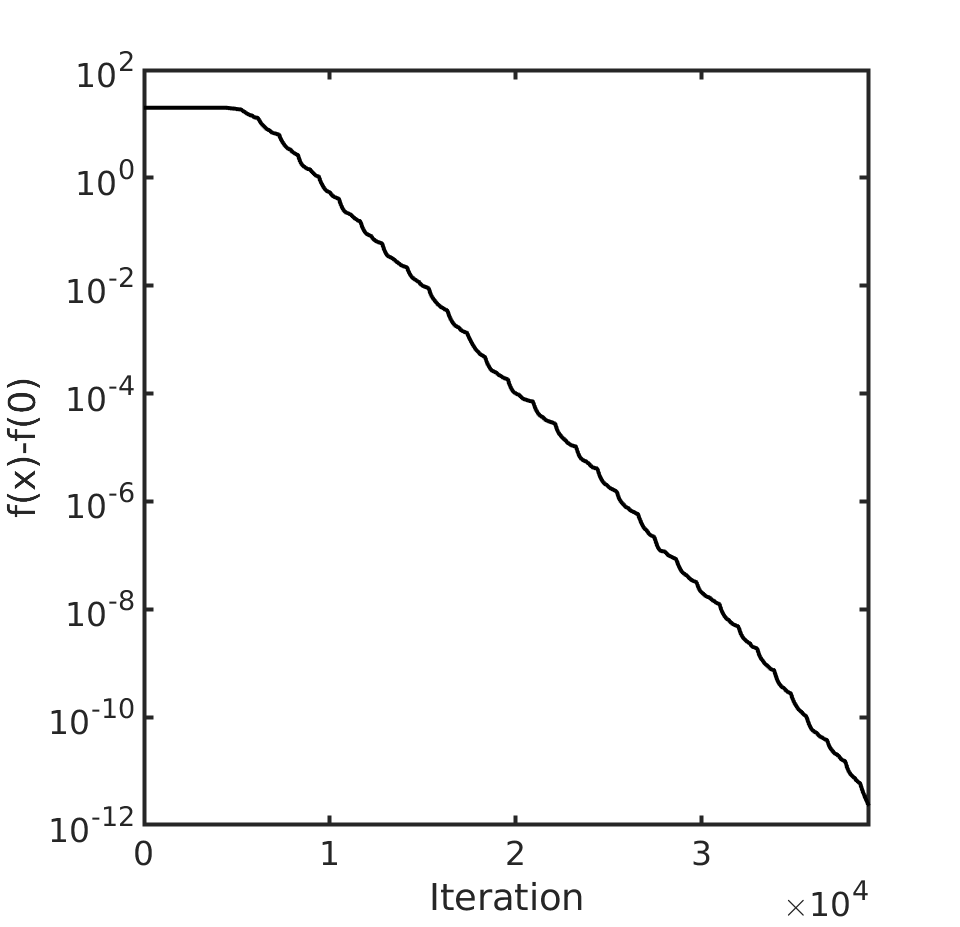
\includegraphics[scale=0.2]{./figures/gauss1000D.png}
	  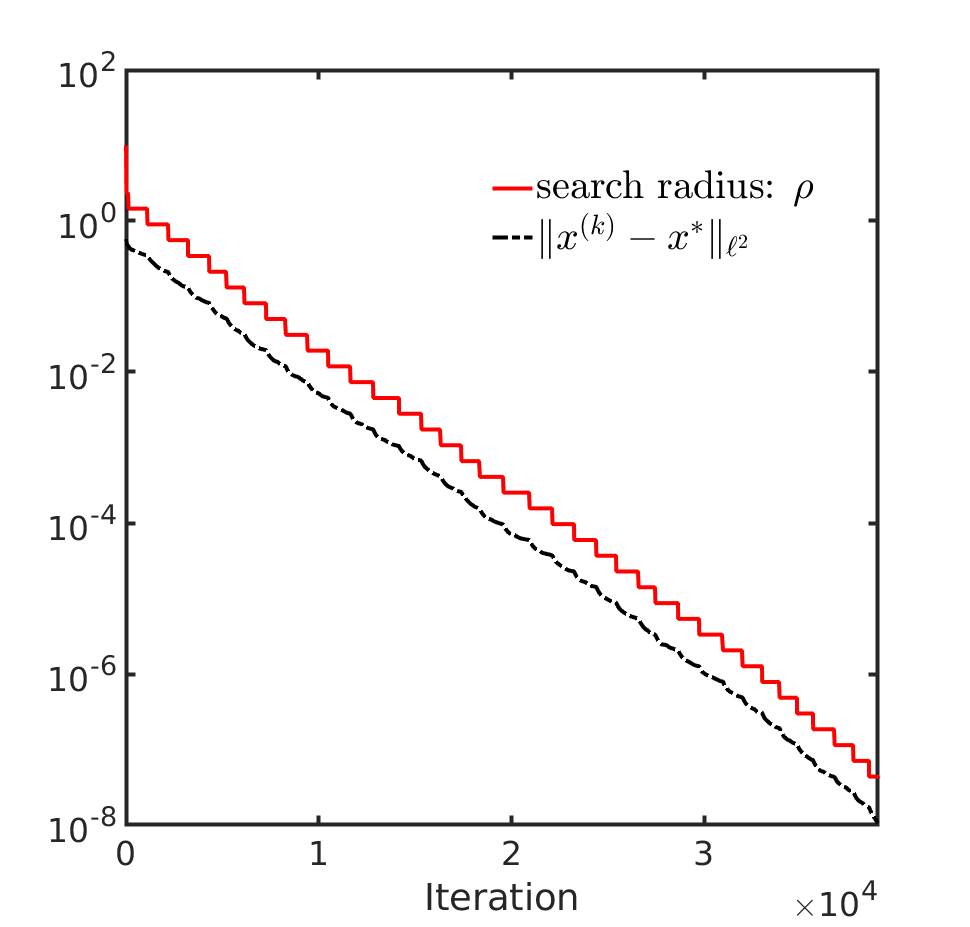
\includegraphics[scale=0.2]{./figures/gauss1000D_dist.png}
\footnotesize{
	\caption{: 
	The initial value was randomly generated in $[-1,1]^{1000}$.
	$\rho_0=0.3$, $\eta=(\sqrt{5}-1)/2$, and $m_{\max}=32$.}
%    The iterations of convergence of the HiCS with
%    constant $\rho=0.3$ for \textcolor{blue}{15D} Gauss function. 
	}
\end{figure}

\end{frame}
%%%%%%%%%%%%%%%%%%%%%%%%%%%%%%%%%%%%%%%%%%%%%%%%%%%%%%%%%%%%%%%%%%%%

%%%%%%%%%%%%%%%%%%%%%%%%%%%%%%%%%%%%%%%%%%%%%%%%%%%%%%%%%%%%%%%%%%%%%
%\begin{frame}{Gauss Function: Iteration}
%    \begin{itemize}
%        \item HiCSa: initial value $x_0 = (6.7, -8.0)$, $\rho=1.0$, $m_{max}=32$.
%    \end{itemize}
%  \movie[externalviewer,label=mymovie,width=1in,height=0.8in,poster]{}{gauss.mp4}
%    \hyperlinkmovie[play]{mymovie}{Movie: Iteration procedure}
%
%\end{frame}
%%%%%%%%%%%%%%%%%%%%%%%%%%%%%%%%%%%%%%%%%%%%%%%%%%%%%%%%%%%%%%%%%%%%%


%%%%%%%%%%%%%%%%%%%%%%%%%%%%%%%%%%%%%%%%%%%%%%%%%%%%%%%%%%%%%%%%%%%%
\subsection{Dennis-Woods Function}

\begin{frame}{Dennis-Woods Function}

\footnotesize{
\begin{align*}
	f(z) = \frac{1}{2}\max\{\|z - c_1 \|^2, \|z - c_2
	\|^2\}, ~~~~ z = (x,y),
	\label{eqn:dwfun}
\end{align*}
where $c_1 = (1,-1)^T$, $c_2 = -c_1$, $\|\cdot\|$ denotes
$\ell^2$-norm.
\begin{itemize}
	\item continuous, strictly convex, but its gradient is
		\textcolor{blue}{discontinuous} along the line $x=y$
\end{itemize}
}
\begin{figure}[!htbp]
	\centering
	  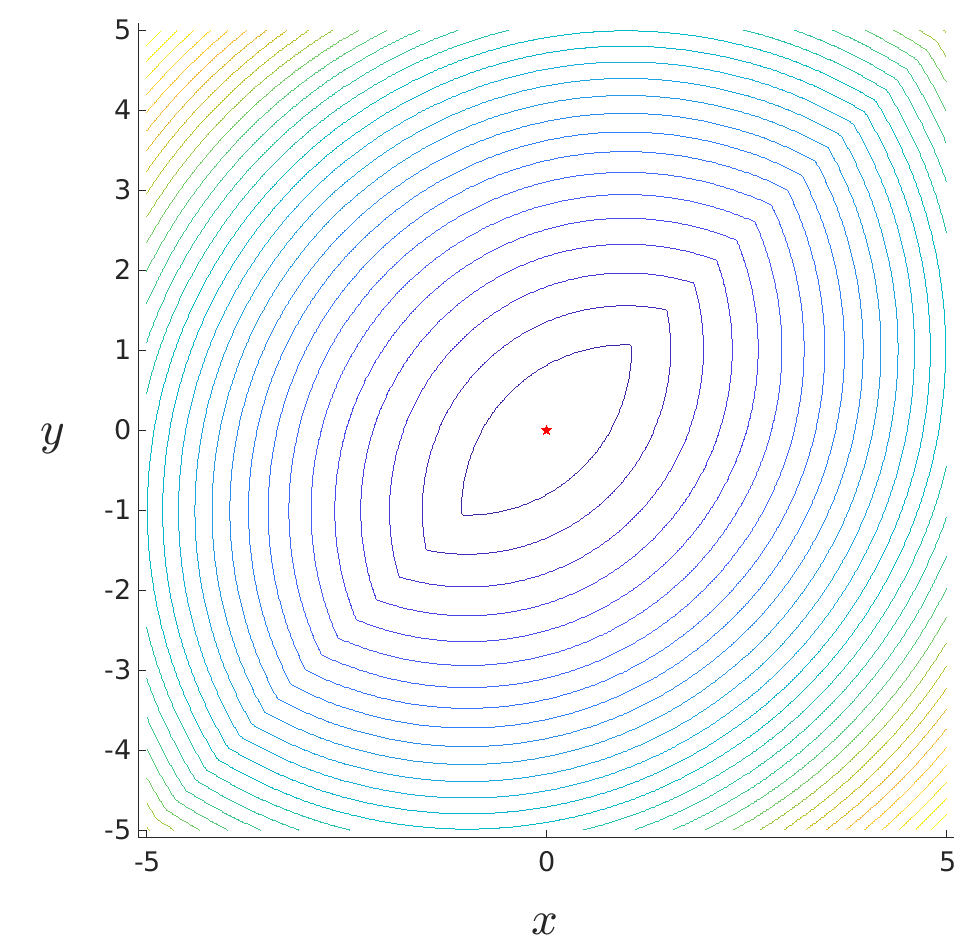
\includegraphics[scale=0.13]{./figures/dWoods.png}
	  \vspace{-0.1cm}
	\footnotesize{
	\caption{: Contours of the variant of the Dennis-Woods function}
	}
\label{fig:dwfun}
\end{figure}
\end{frame}
%%%%%%%%%%%%%%%%%%%%%%%%%%%%%%%%%%%%%%%%%%%%%%%%%%%%%%%%%%%%%%%%%%%%

%%%%%%%%%%%%%%%%%%%%%%%%%%%%%%%%%%%%%%%%%%%%%%%%%%%%%%%%%%%%%%%%%%%%
\begin{frame}{Dennis-Woods Function}
\normalsize{
	\begin{itemize}
		\item HiCS can capture the minimizer within finite-step iterations
	\end{itemize}
	}
\begin{figure}[!htbp]
	\centering
	  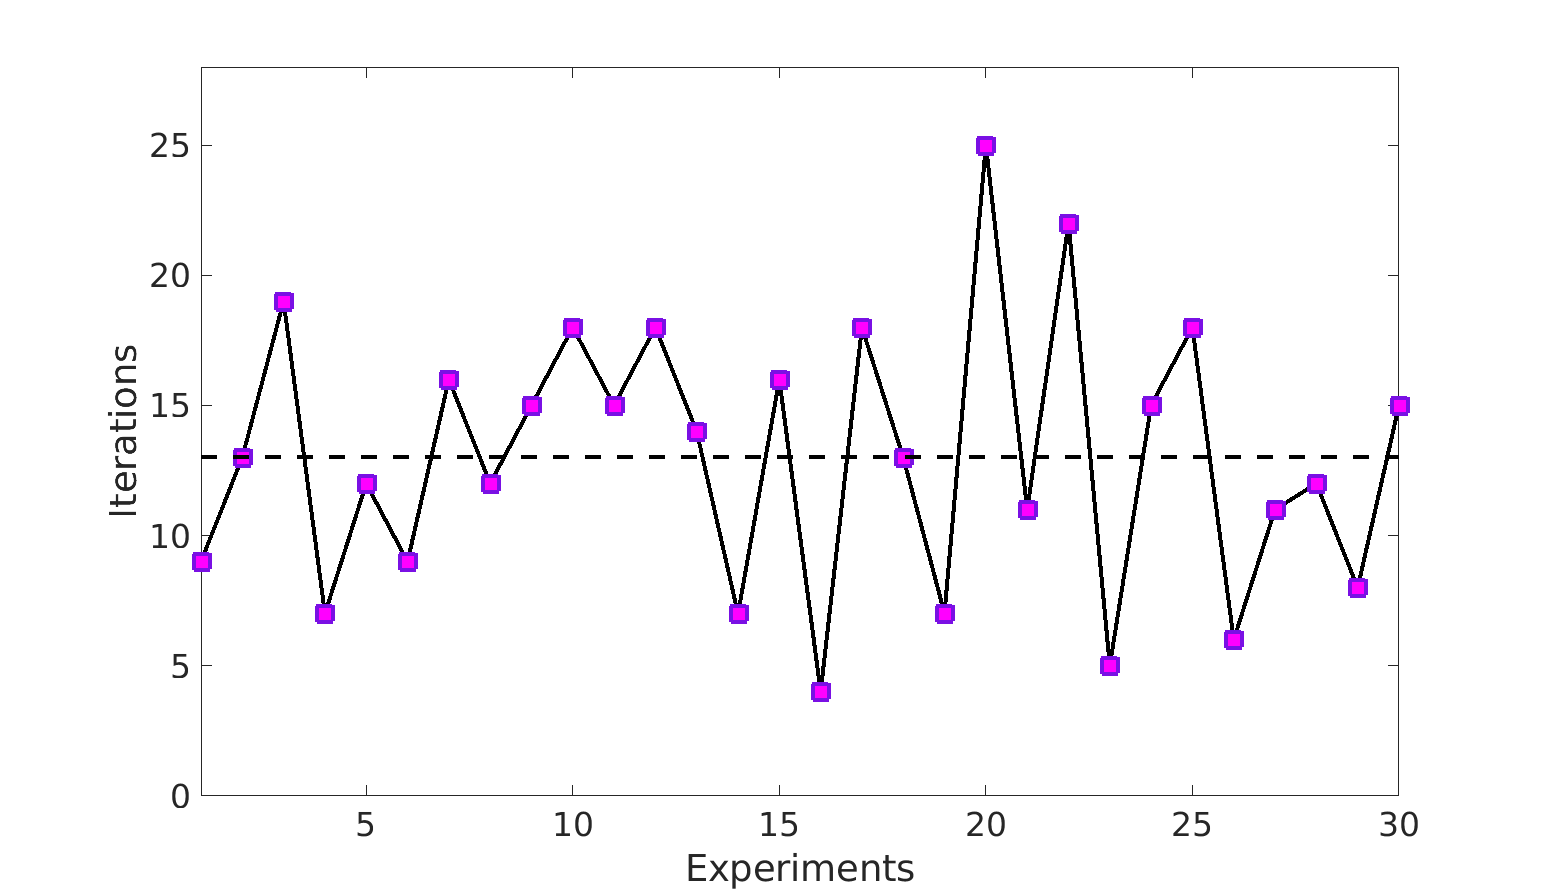
\includegraphics[scale=0.22]{./figures/dwoodrand.png}
	\caption{:
\footnotesize{
	The iterations of convergence of the HiCS with
	constant $\rho=0.5$ for 2D Gauss function. The initial
	values were randomly generated in $[-5,5]^2$.}
}
\label{fig:dwfunrand}
\end{figure}
\end{frame}
%%%%%%%%%%%%%%%%%%%%%%%%%%%%%%%%%%%%%%%%%%%%%%%%%%%%%%%%%%%%%%%%%%%%

%%%%%%%%%%%%%%%%%%%%%%%%%%%%%%%%%%%%%%%%%%%%%%%%%%%%%%%%%%%%%%%%%%%%%
%\begin{frame}{Dennis-Woods Function: Iteration}
%    \begin{itemize}
%        \item HiCS: initial value $x_0 = (3.2, 1.5)$, $\rho=0.5$, $m_{max}=32$.
%    \end{itemize}
%
%  \movie[externalviewer,label=mymovie,width=1in,height=0.8in,poster]{}{dwoods.mp4}
%    \hyperlinkmovie[play]{mymovie}{\textcolor{blue}{Movie: Iteration procedure}}
%\end{frame}
%%%%%%%%%%%%%%%%%%%%%%%%%%%%%%%%%%%%%%%%%%%%%%%%%%%%%%%%%%%%%%%%%%%%%


%%%%%%%%%%%%%%%%%%%%%%%%%%%%%%%%%%%%%%%%%%%%%%%%%%%%%%%%%%%%%%%%%%%%
\begin{frame}{Dennis-Woods Function}
	\begin{itemize}
		\item HiCS: initial value $x_0 = (3.2, 1.5)$, $\rho=0.5$, $m_{max}=32$.
	\end{itemize}
\footnotesize{
\begin{table}[!htbp]
%\caption{: Iteration information}
\begin{center}
\begin{tabular}{|c|c|c|}
 \hline
    Iter. & $\ell^2$-distance &  Fun. Val.
 \\\hline
 \makecell{ 1 (1-15) } & \makecell{ 3.53412 \\ $\downarrow$ \\ 3.79272e-01 }
 & \makecell{8.94500  \\ $\downarrow$ \\1.13987 }
 \\\hline
 3  &1.34218e-01 & 1.12407
 \\\hline
 15  & \textcolor{blue}{3.89309e-01} & 1.09854
 \\\hline
 32  & 1.12185e-01 &  1.02906
 \\\hline
\end{tabular}
\end{center}
\end{table}
}
\pause
\vspace{-1cm}
\normalsize{
  \movie[externalviewer,label=mymovie,width=1in,height=0.8in,poster]{}{./figures/dw1.avi}
  \hyperlinkmovie[play]{mymovie}{\textcolor{blue}{Movie: Iteration procedure}}
}
\end{frame}
%%%%%%%%%%%%%%%%%%%%%%%%%%%%%%%%%%%%%%%%%%%%%%%%%%%%%%%%%%%%%%%%%%%%

%%%%%%%%%%%%%%%%%%%%%%%%%%%%%%%%%%%%%%%%%%%%%%%%%%%%%%%%%%%%%%%%%%%%
\begin{frame}{Dennis-Woods Function: Comparison}
\begin{itemize}
	\item The popular Nelder-Mead simplex algorithm \textcolor{blue}{fails}
	\item The coordinate-search (CS) method (with predetermined search
		directions $\mathcal{D}_\oplus$) \textcolor{blue}{stalls}
\end{itemize}
\begin{figure}[!htbp]
	\centering
	  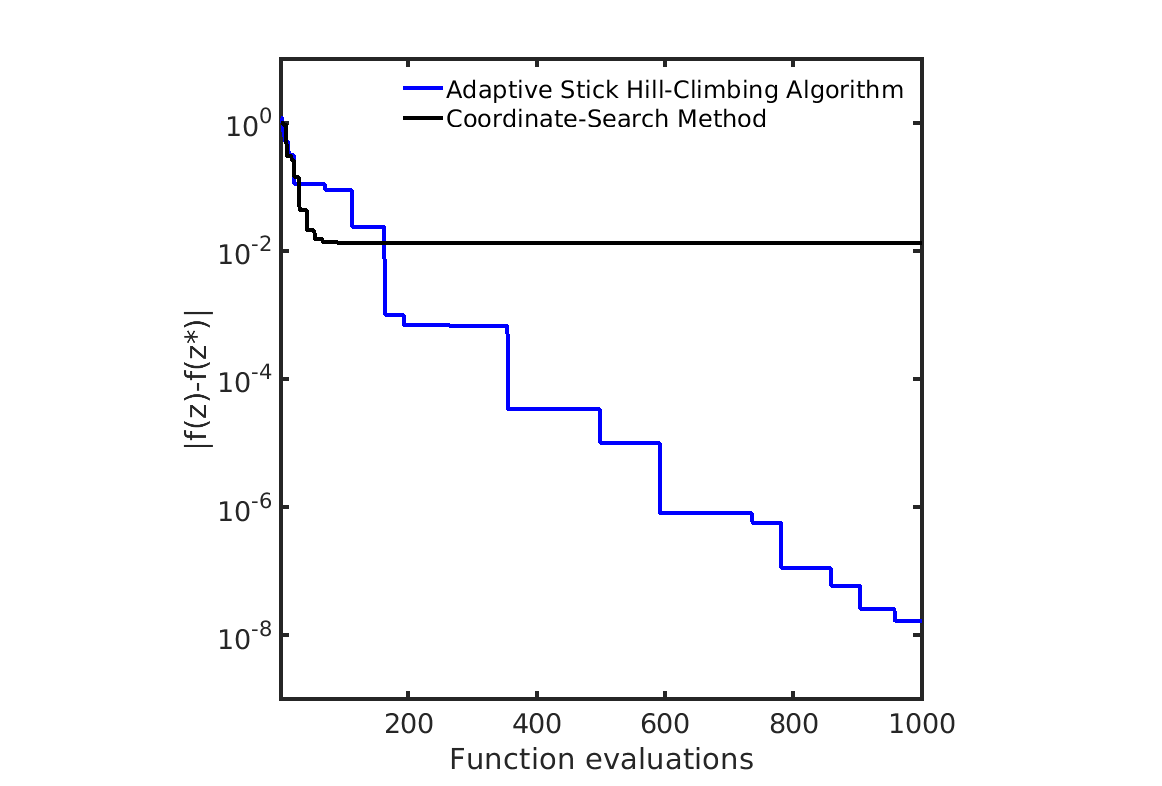
\includegraphics[scale=0.17]{./figures/dwoods_cmp.png}
	  \caption{
	  \footnotesize{
	  Application of the adaptive stick hill-climbing method
	  ($m_{\max}=8$) and the CS method with
	  $\mathcal{D}_{\oplus}=\{(1,0), (0,1), (-1,0), (0,-1)\}$,
	  starting from $x_0=(1.1, 0.9)$.
	  The initial search radii are both $\rho_0 = 1.0$,
	  the control factor $\eta=0.5$.}
	  }
\label{fig:dwfun:cmp}
\end{figure}
\end{frame}
%%%%%%%%%%%%%%%%%%%%%%%%%%%%%%%%%%%%%%%%%%%%%%%%%%%%%%%%%%%%%%%%%%%%

\subsection{Ackley Function}

%%%%%%%%%%%%%%%%%%%%%%%%%%%%%%%%%%%%%%%%%%%%%%%%%%%%%%%%%%%%%%%%%%%%
\begin{frame}{Ackley Function}
\footnotesize{
\begin{itemize}
	\item Many local minima and a unique global
minimum $0$ with $f(0)=0$.
	\item Non-convex
\end{itemize}
\vspace{-0.2cm}
\begin{align*}
	f(\bmx) =
	-20\cdot\exp\left(-0.2\cdot\sqrt{\frac{1}{n}\sum_{i=1}^n
	x_i^2}~\right)-
	\exp\left(\frac{1}{n}\sum_{i=1}^n \cos(2\pi x_i)\right)+20+e
\end{align*}
}
%$n$ is the dimension.
\vspace{-0.4cm}
\begin{figure}[!htbp]
	\centering
	  \includegraphics[scale=0.2]{./figures/ackley.png}
	  \caption{: 2D Ackley function}
\end{figure}
\end{frame}
%%%%%%%%%%%%%%%%%%%%%%%%%%%%%%%%%%%%%%%%%%%%%%%%%%%%%%%%%%%%%%%%%%%%

%%%%%%%%%%%%%%%%%%%%%%%%%%%%%%%%%%%%%%%%%%%%%%%%%%%%%%%%%%%%%%%%%%%%
\begin{frame}{Ackley Function: 2D}
	\begin{itemize}
		\item HiCSa: initial value $x_0 = (6.12, 5.426)$, $\rho=2.5$
	\end{itemize}

  \movie[externalviewer,label=mymovie,width=1in,height=0.8in,poster]{}{./figures/ackley1.avi}
  \hyperlinkmovie[play]{mymovie}{\textcolor{blue}{Movie: Iteration procedure}}
\end{frame}
%%%%%%%%%%%%%%%%%%%%%%%%%%%%%%%%%%%%%%%%%%%%%%%%%%%%%%%%%%%%%%%%%%%%


%%%%%%%%%%%%%%%%%%%%%%%%%%%%%%%%%%%%%%%%%%%%%%%%%%%%%%%%%%%%%%%%%%%%%
%\begin{frame}{Ackley Function: 2D}
%
%\footnotesize{
%    $\bullet$ Apply HiCSa to 2D Ackley.
%        The initial value is $x_0=(4.1,3.4)$, $\rho_0=2.5$, $\eta=0.5$, $m_{max}=32$
%    }
%    \vspace{0.3cm}
%\scriptsize{
%\begin{table}[!htbp]
%%\caption{: Iteration information}
%\begin{center}
%\vspace{-0.5cm}
%\begin{tabular}{|c|c|c||c|c|c|}
% \hline
% $\rho$ &  Iter. & $\ell^2$-distance
% & $\rho$ &  Iter. & $\ell^2$-distance
% \\\hline
% $2.5$ & \makecell{ 1 (1-5) \\  \\ 32} & \makecell{ 8.1789899132e+00
% \\ $\downarrow$ \\ 1.0770647084e+00 }
% & 7.812500e-02  & 32  &  2.8671697567e-02
% \\\hline
% $1.25$ & \makecell{ 1 \\ 1 \\ 6 \\ 3
% \\ 15 \\ 32} & \makecell{
%1.0770647084e+00
%\\
%7.5511786386e-01
%\\
%9.0643428768e-01
%\\
%3.7558136376e-01
%\\
%\textcolor{blue}{8.8719307270e-01}
%\\
%3.6508163385e-01
% }
% & 3.906250e-02& \makecell{1 \\ 32} & \makecell{
%2.8671697567e-02
%\\
%1.0415421005e-02
%}
%\\\hline
% $0.625$ & \makecell{ 1  \\ 2 \\ 32} & \makecell{
%3.6508163385e-01
%\\
%3.3018360271e-01
%\\
%2.9552513683e-01
% }
% & 1.953125e-02& \makecell{1 \\ 32} & \makecell{
%1.0415421005e-02
%\\
%9.1544465411e-03
% }
% \\\hline
% $0.3125$ & \makecell{ 1  \\ 32} & \makecell{
%2.9552513683e-01
%\\
%1.4349657932e-01
% }
%& $\downarrow$ & $\downarrow$ & $\downarrow$
% \\\hline
% 0.15625 & \makecell{  1 \\ 32 }
% & \makecell{
% 1.4349657932e-01  \\ 2.8671697567e-02
% }
% & 1.907349e-05 & \makecell{1 \\ 32}
% & \makecell{
%1.4744333518e-05 \\
%7.4878517018e-06
% }
% \\\hline
%\end{tabular}
%\end{center}
%\end{table}
%}
%\end{frame}
%%%%%%%%%%%%%%%%%%%%%%%%%%%%%%%%%%%%%%%%%%%%%%%%%%%%%%%%%%%%%%%%%%%%%

%%%%%%%%%%%%%%%%%%%%%%%%%%%%%%%%%%%%%%%%%%%%%%%%%%%%%%%%%%%%%%%%%%%
\begin{frame}{Ackley Function: 2D}
\begin{itemize}
	\item Has potential to distinguish different minima
\end{itemize}
\begin{figure}[!htbp]
	\centering
	  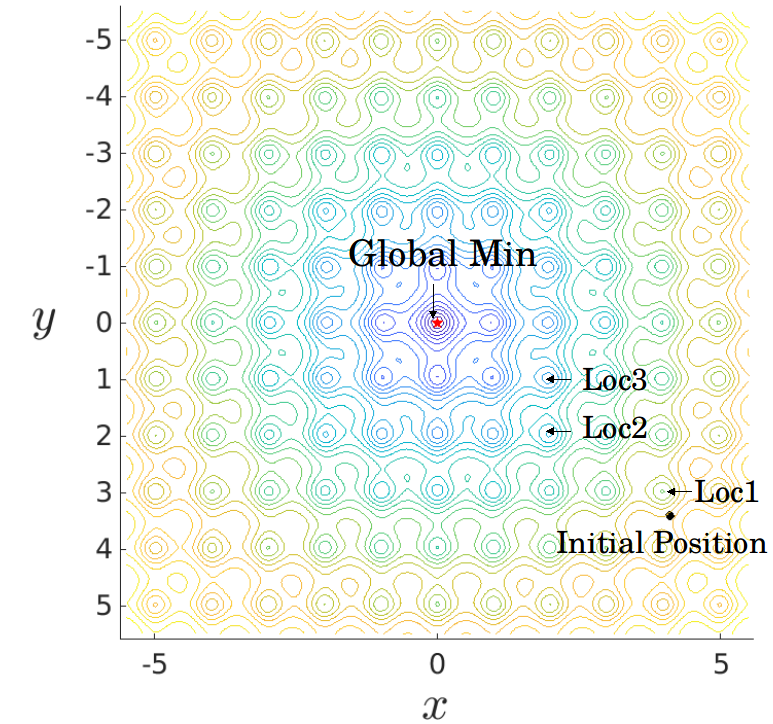
\includegraphics[scale=0.18]{./figures/ackley_LG.png}
\end{figure}
\vspace{-0.6cm}
\footnotesize{
\begin{table}[!htbp]
\caption{\label{tab:ackley:r}: The convergent results and required
iterations with differently \textcolor{blue}{constant $\rho$}
starting from the initial state $(x_0, y_0)=(4.1, 3.4)$.}
\begin{center}
\begin{tabular}{|c|c|c|c|c|c|c|c|}
 \hline
 $\rho$ & 0.1 & 0.3 & 0.5 & 0.55 & 0.58 &  0.6 & 1.0
 \\\hline
 Iter. & 7   & 3   &  2  & 6 & 7 & 15 & 7
 \\\hline
 Min. & $\rm{Loc_1}$ & $\rm{Loc_1}$ & $\rm{Loc_1}$ & $\rm{Loc_2}$
	& $\rm{Loc_3}$ & Global & Global
 \\\hline
\end{tabular}
\end{center}
\end{table}
}
\end{frame}
%%%%%%%%%%%%%%%%%%%%%%%%%%%%%%%%%%%%%%%%%%%%%%%%%%%%%%%%%%%%%%%%%%%%

%%%%%%%%%%%%%%%%%%%%%%%%%%%%%%%%%%%%%%%%%%%%%%%%%%%%%%%%%%%%%%%%%%%%
\begin{frame}{Ackley Function: 100D}
\footnotesize{
	\begin{itemize}
		\item We apply HiCS to 100D Ackley with constant $\rho_0=2$.
		The initial value is randomly generated in $[-10,10]^{100}$.
		$m_{\max}=32$.
	\end{itemize}
	\vspace{-0.5cm}
	}
\footnotesize{
\begin{table}[!htbp]
%\caption{Iteration information}
\begin{center}
\begin{tabular}{|c|c|c|}
 \hline
    Iter. & $\ell^2$-distance &  Fun. Val.
 \\\hline
 \makecell{ 1 (1-353) } & \makecell{ 43.76984 \\ $\downarrow$ \\
 5.67057 }
 & \makecell{  13.40276 \\ $\downarrow$ \\ 3.65003 }
 \\\hline
 3  &\textcolor{blue}{5.76768} & 3.64961
 \\\hline
 5  & \textcolor{blue}{5.84103} &3.64579
 \\\hline
  5  & 5.75717 &3.63706
 \\\hline
1  & 5.72732  & 3.63154
 \\\hline
 1 &   5.68106  & 3.63021
 \\\hline
 6 &   5.67458  & 3.60655
 \\\hline
 12 &  5.76181  &  3.60569
 \\\hline
 5  & \textcolor{blue}{5.84496}  & 3.59674
 \\\hline
1  & 5.76528  & 3.59377
 \\\hline
1  & 5.71754  & 3.59277
 \\\hline
 2  & \textcolor{blue}{5.90908} &  3.59054
 \\\hline
 32 ($m_{max}$) & \textcolor{blue}{5.93767} &  3.58252
 \\\hline
\end{tabular}
\end{center}
\end{table}
}
\end{frame}
%%%%%%%%%%%%%%%%%%%%%%%%%%%%%%%%%%%%%%%%%%%%%%%%%%%%%%%%%%%%%%%%%%%%


%%%%%%%%%%%%%%%%%%%%%%%%%%%%%%%%%%%%%%%%%%%%%%%%%%%%%%%%%%%%%%%%%%%%
\begin{frame}{Ackley Function: 100D}
	\begin{itemize}
		\item We can continue apply HiCSa ($\eta=0.5$) to 100D Ackley.
	\end{itemize}
\begin{figure}[!htbp]
	\centering
	  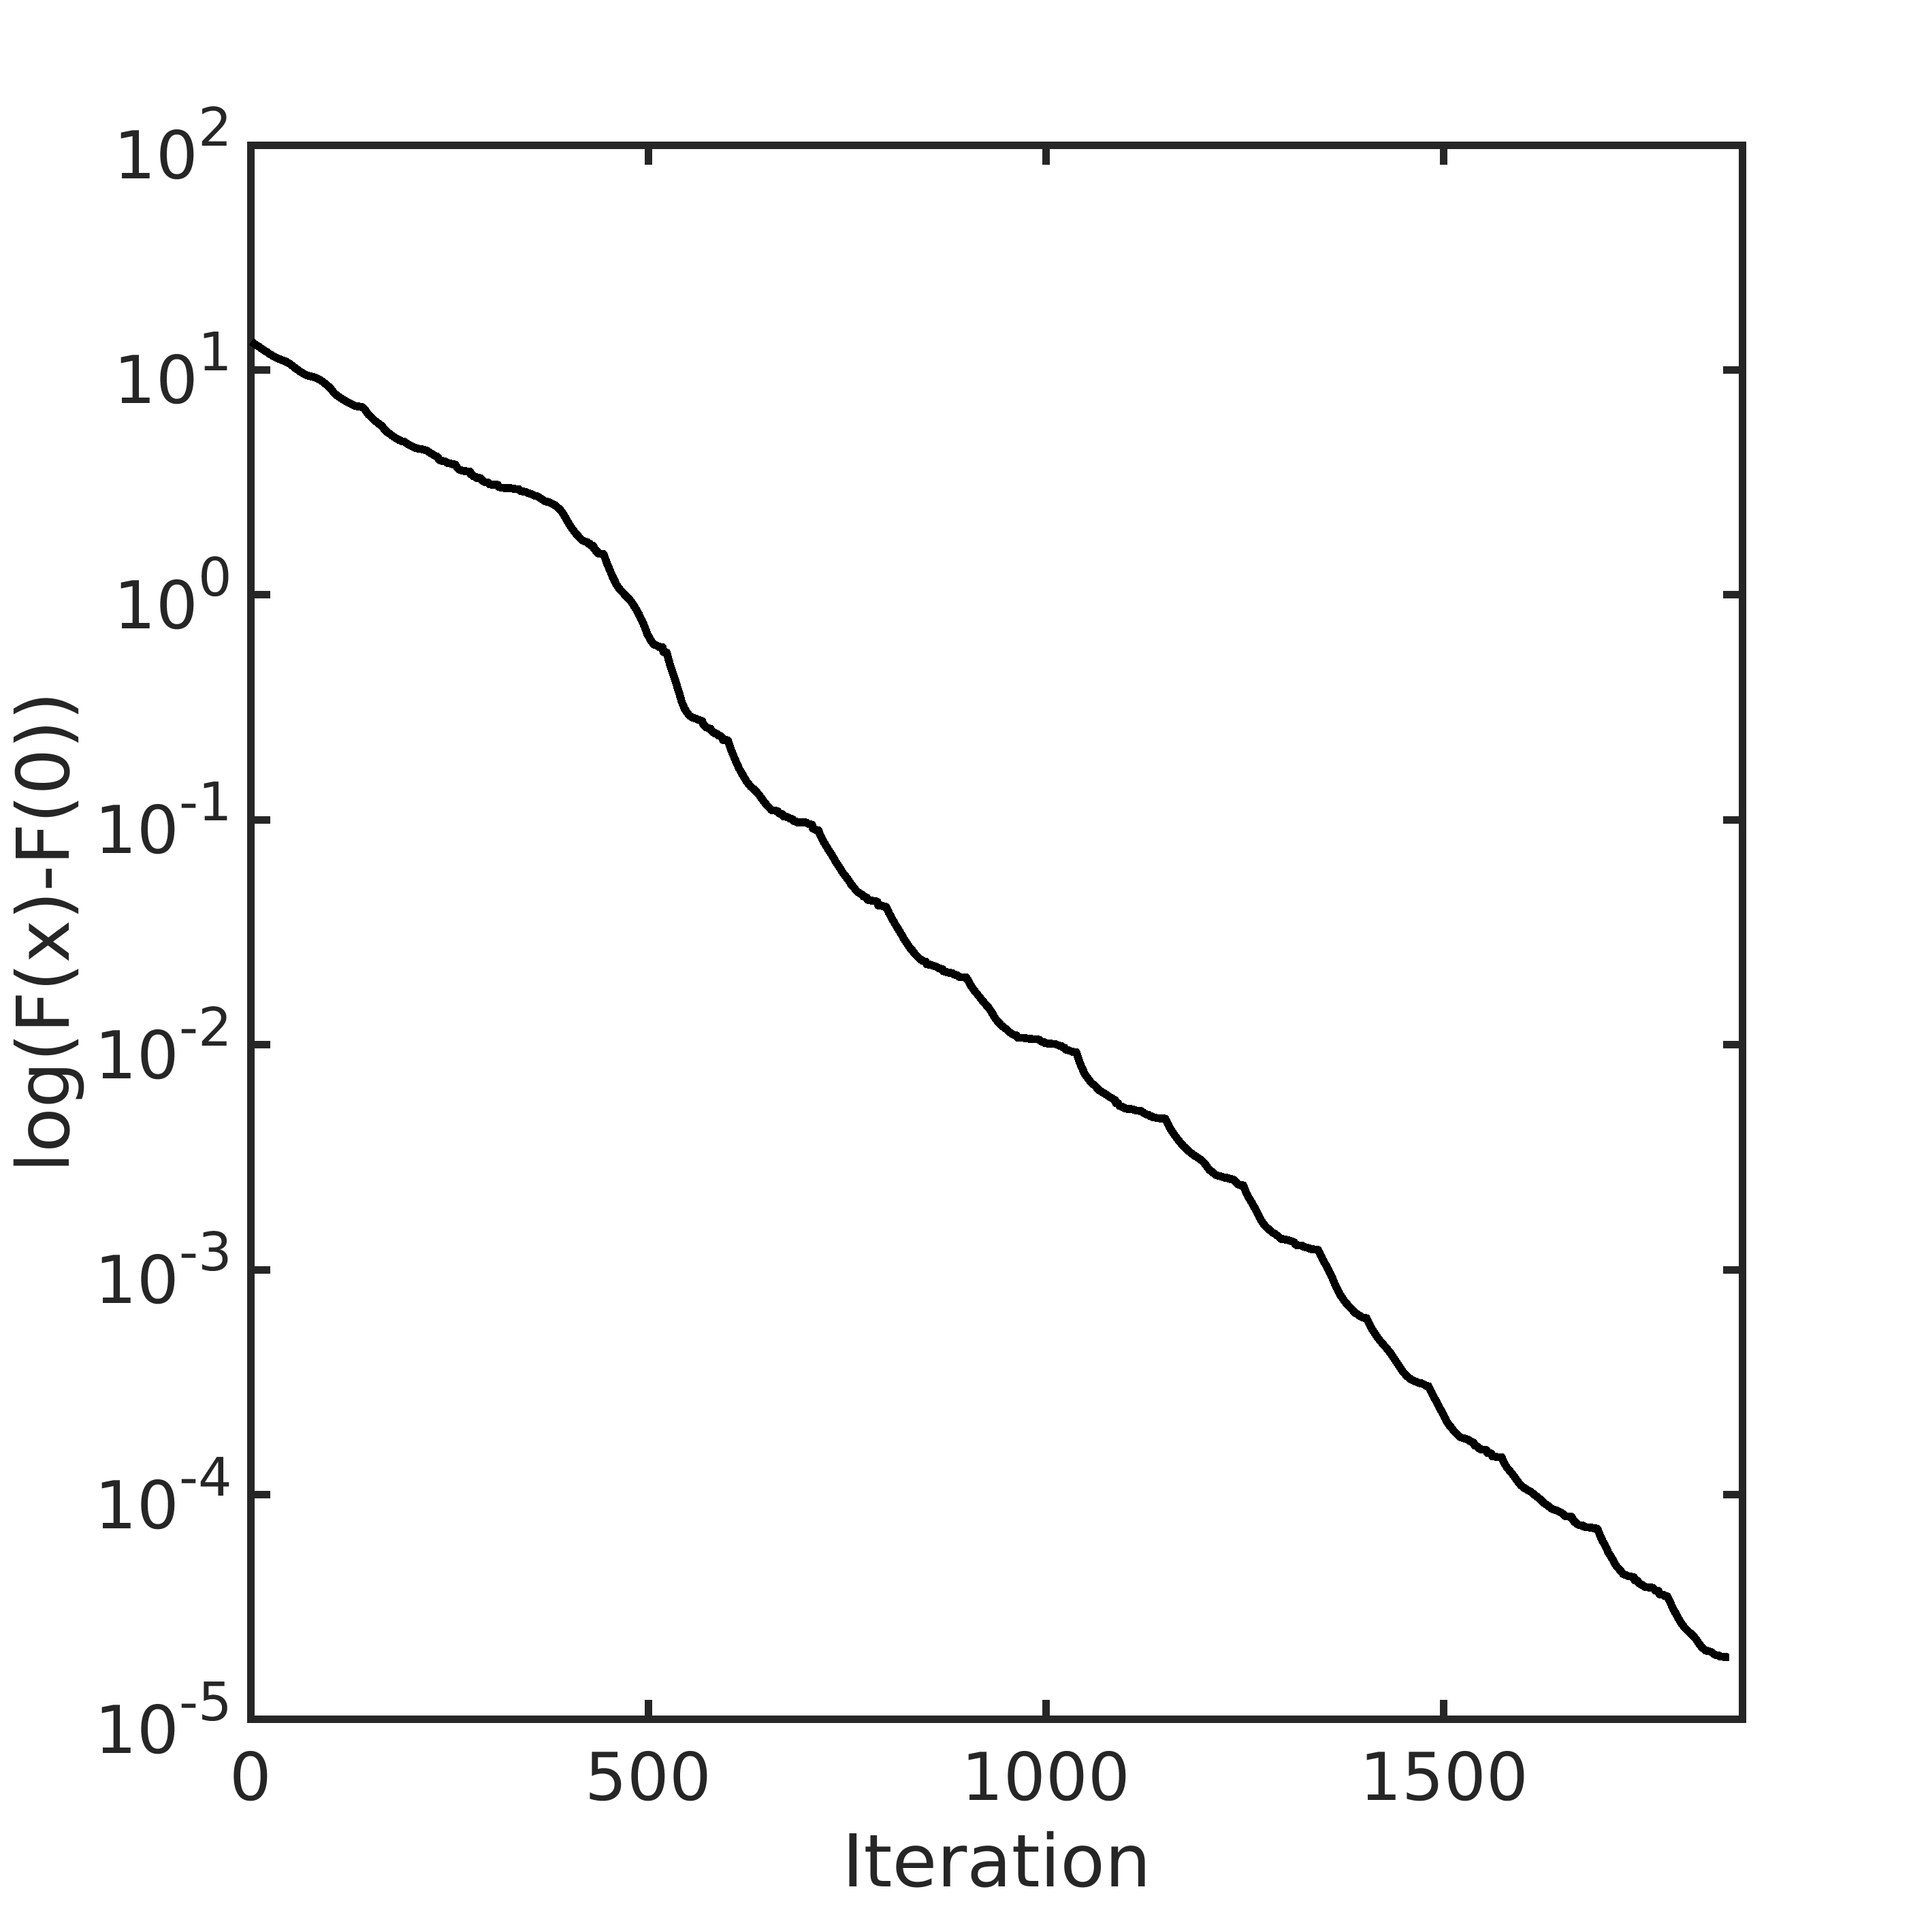
\includegraphics[scale=0.2]{./figures/ackley100D.png}
	  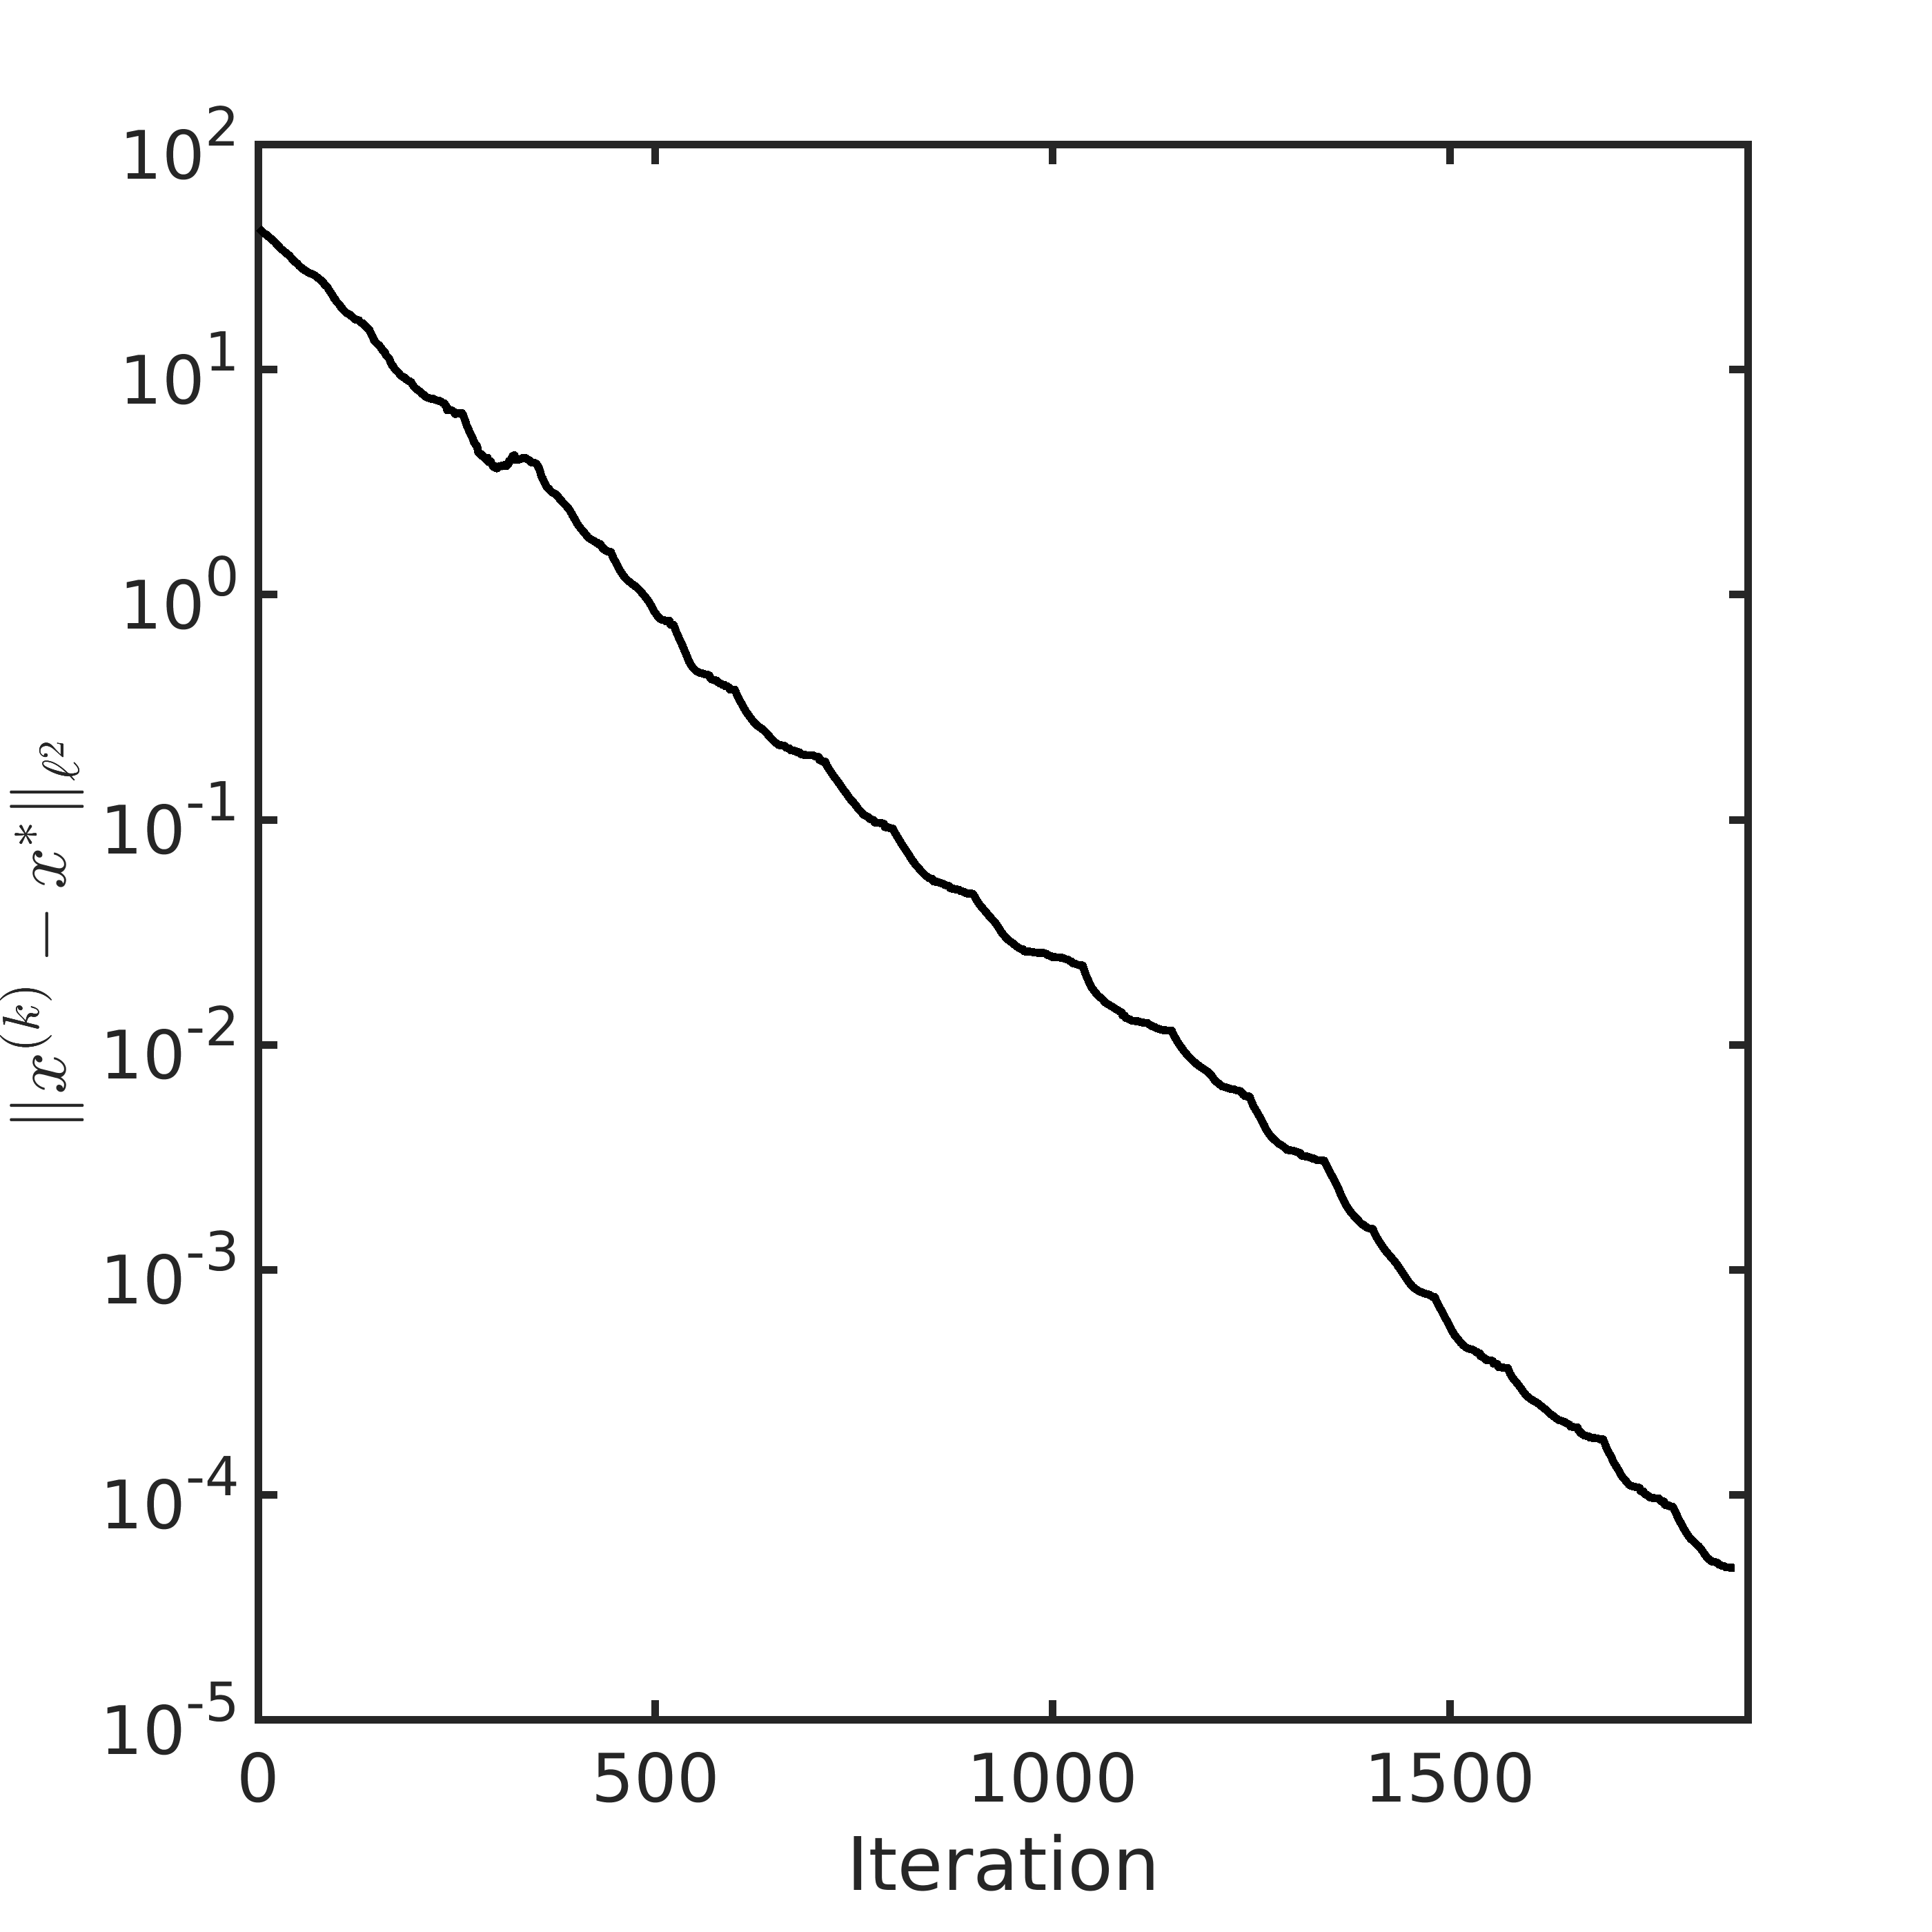
\includegraphics[scale=0.2]{./figures/ackley100D_dist.png}
\end{figure}
\end{frame}
%%%%%%%%%%%%%%%%%%%%%%%%%%%%%%%%%%%%%%%%%%%%%%%%%%%%%%%%%%%%%%%%%%%%


%%%%%%%%%%%%%%%%%%%%%%%%%%%%%%%%%%%%%%%%%%%%%%%%%%%%%%%%%%%%%%%%%%%%
\begin{frame}{Ackley Function: 100D}
\footnotesize{
	\begin{itemize}
		\item HiCSa can capture different local minima with
			smaller $\rho_0$.
		\item Setup: the start point is randonly generated in
			$[-5,5]^{\textcolor{blue}{100}}$, $m_{\max}=32$,
			$\eta=0.5$ and $r<1.0\times 10^{-14}$.
	\end{itemize}
}
\vspace{-0.6cm}
\begin{columns}[c]
	\column{6cm}
\begin{figure}[!htbp]
	\centering
	  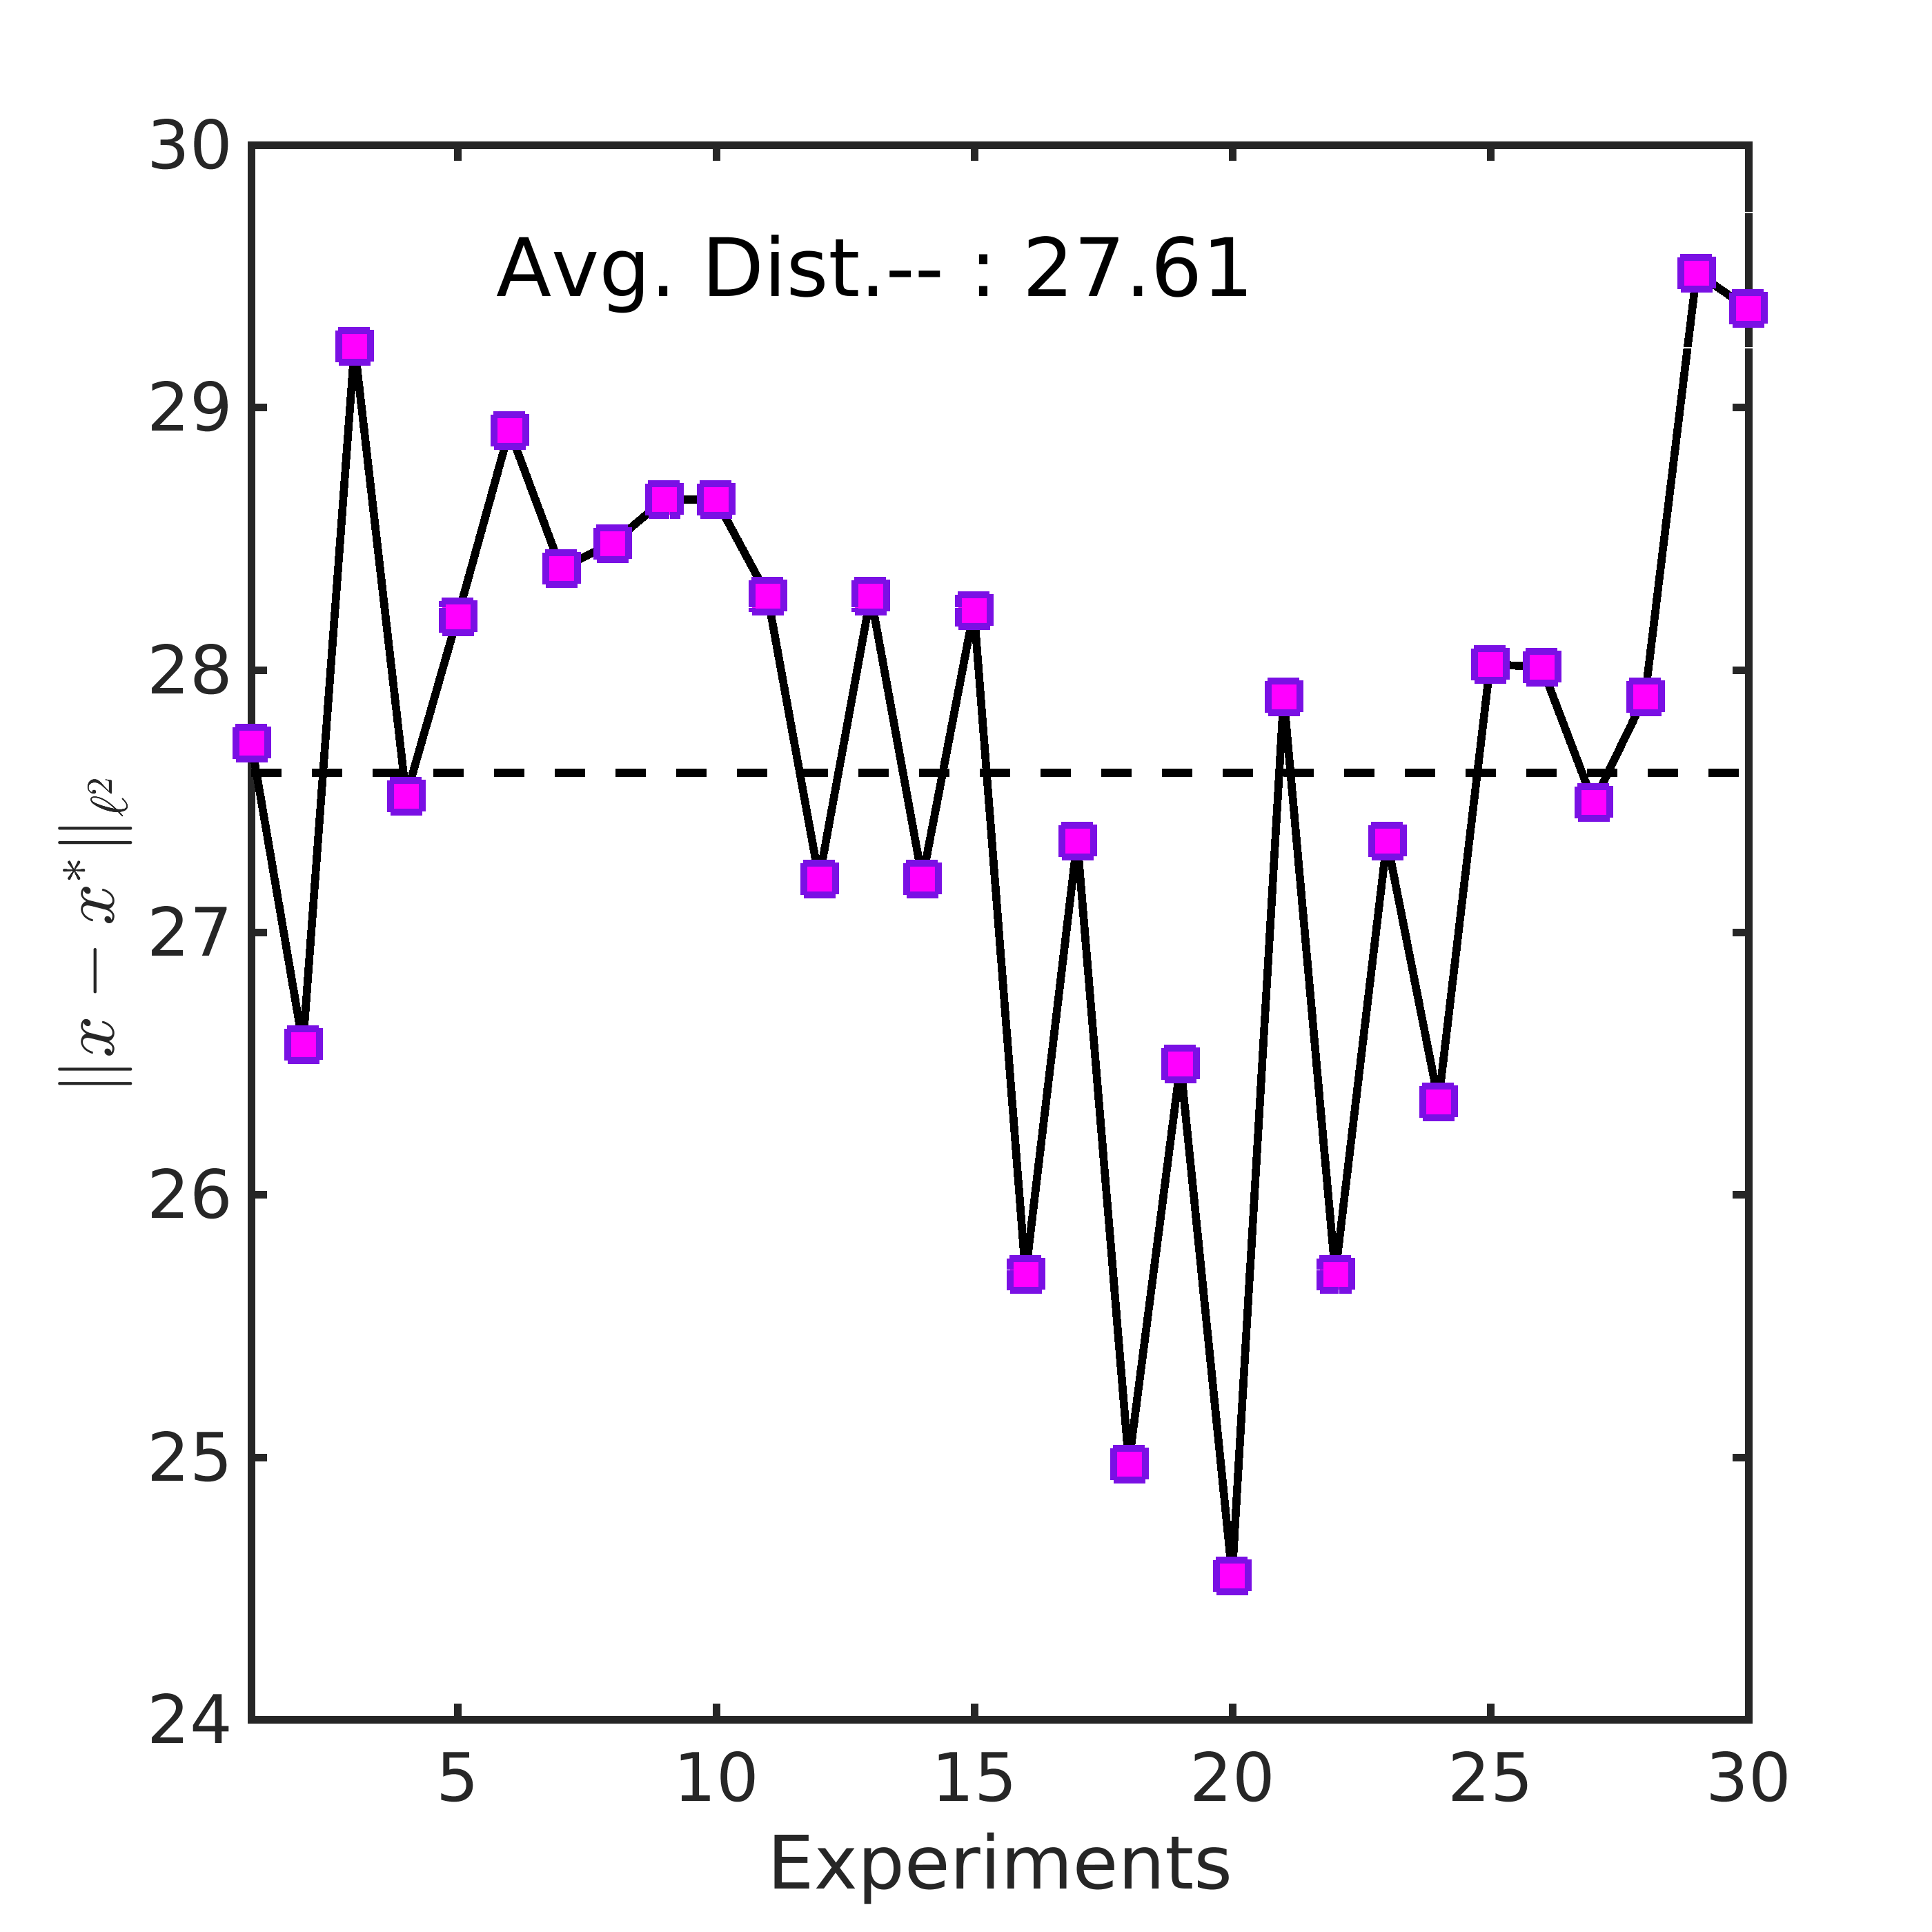
\includegraphics[scale=0.1]{./figures/ackley100Drandr0_05_dist.png}
	  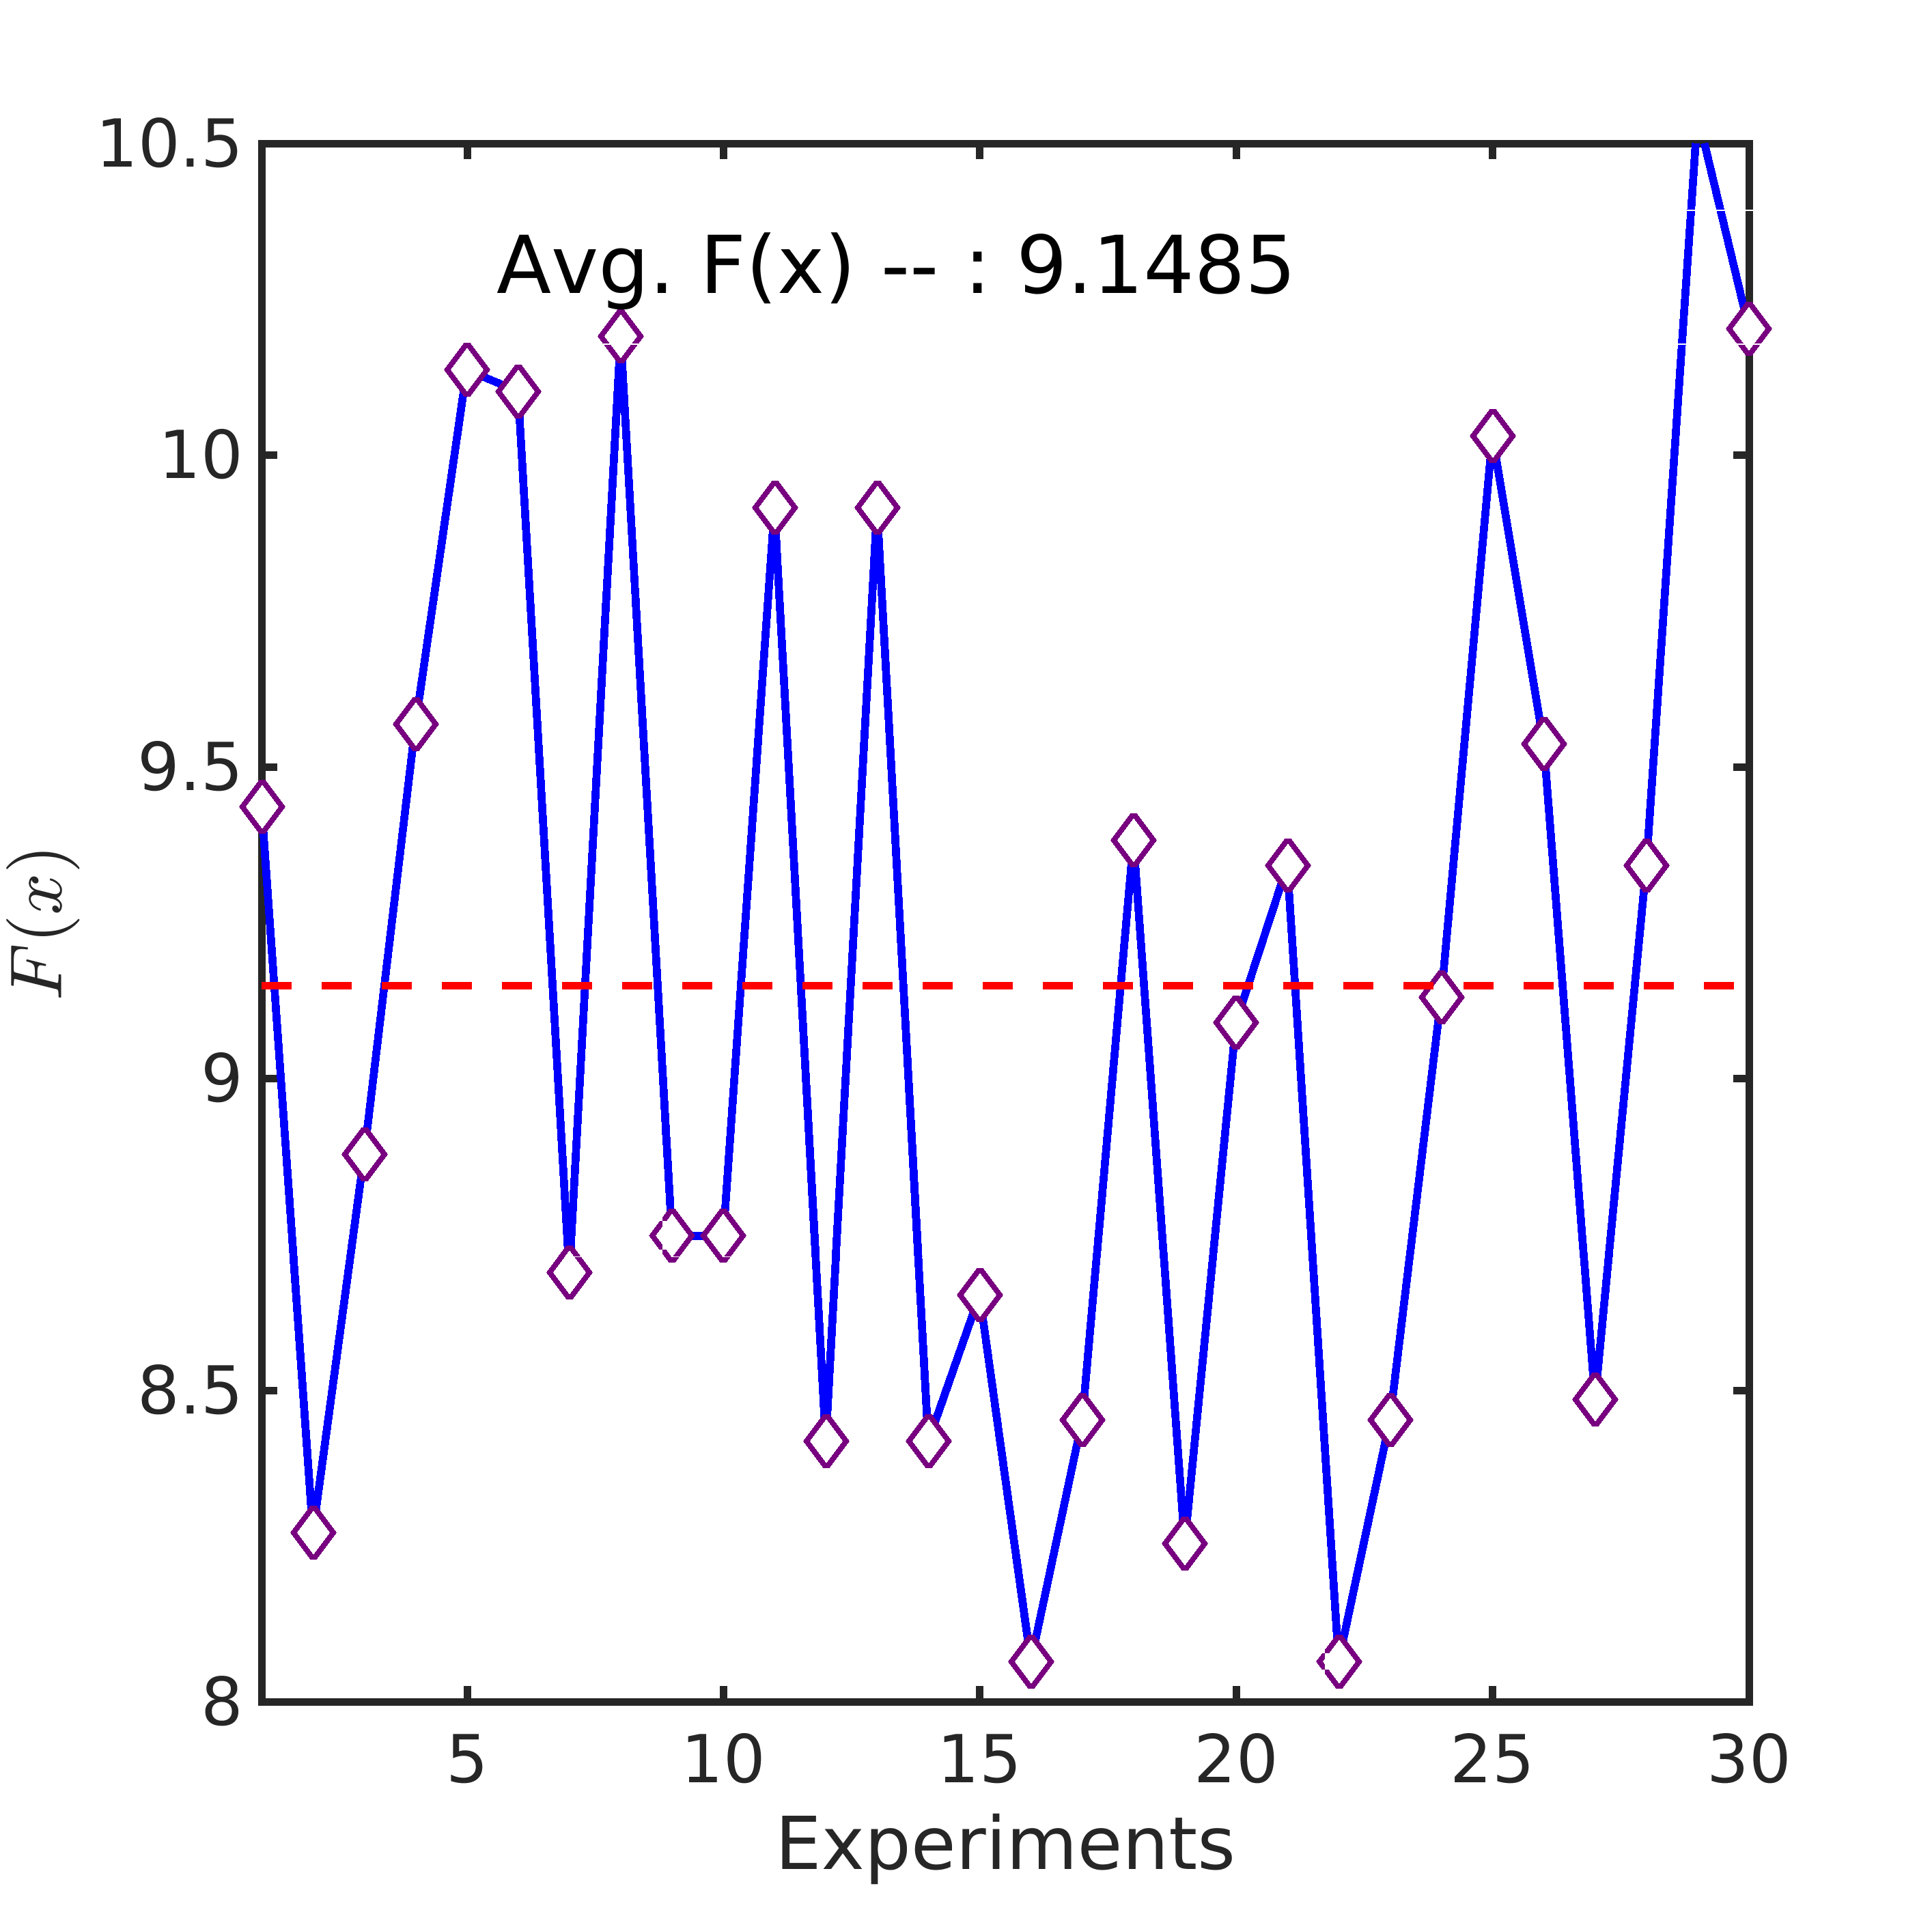
\includegraphics[scale=0.1]{./figures/ackley100Drandr0_05_val.png}
	  \vspace{-0.2cm}
	  \footnotesize{ \caption{: $\rho_0=0.05$.} }
\end{figure}
\column{6cm} 
\begin{figure}[!htbp]
	\centering
	  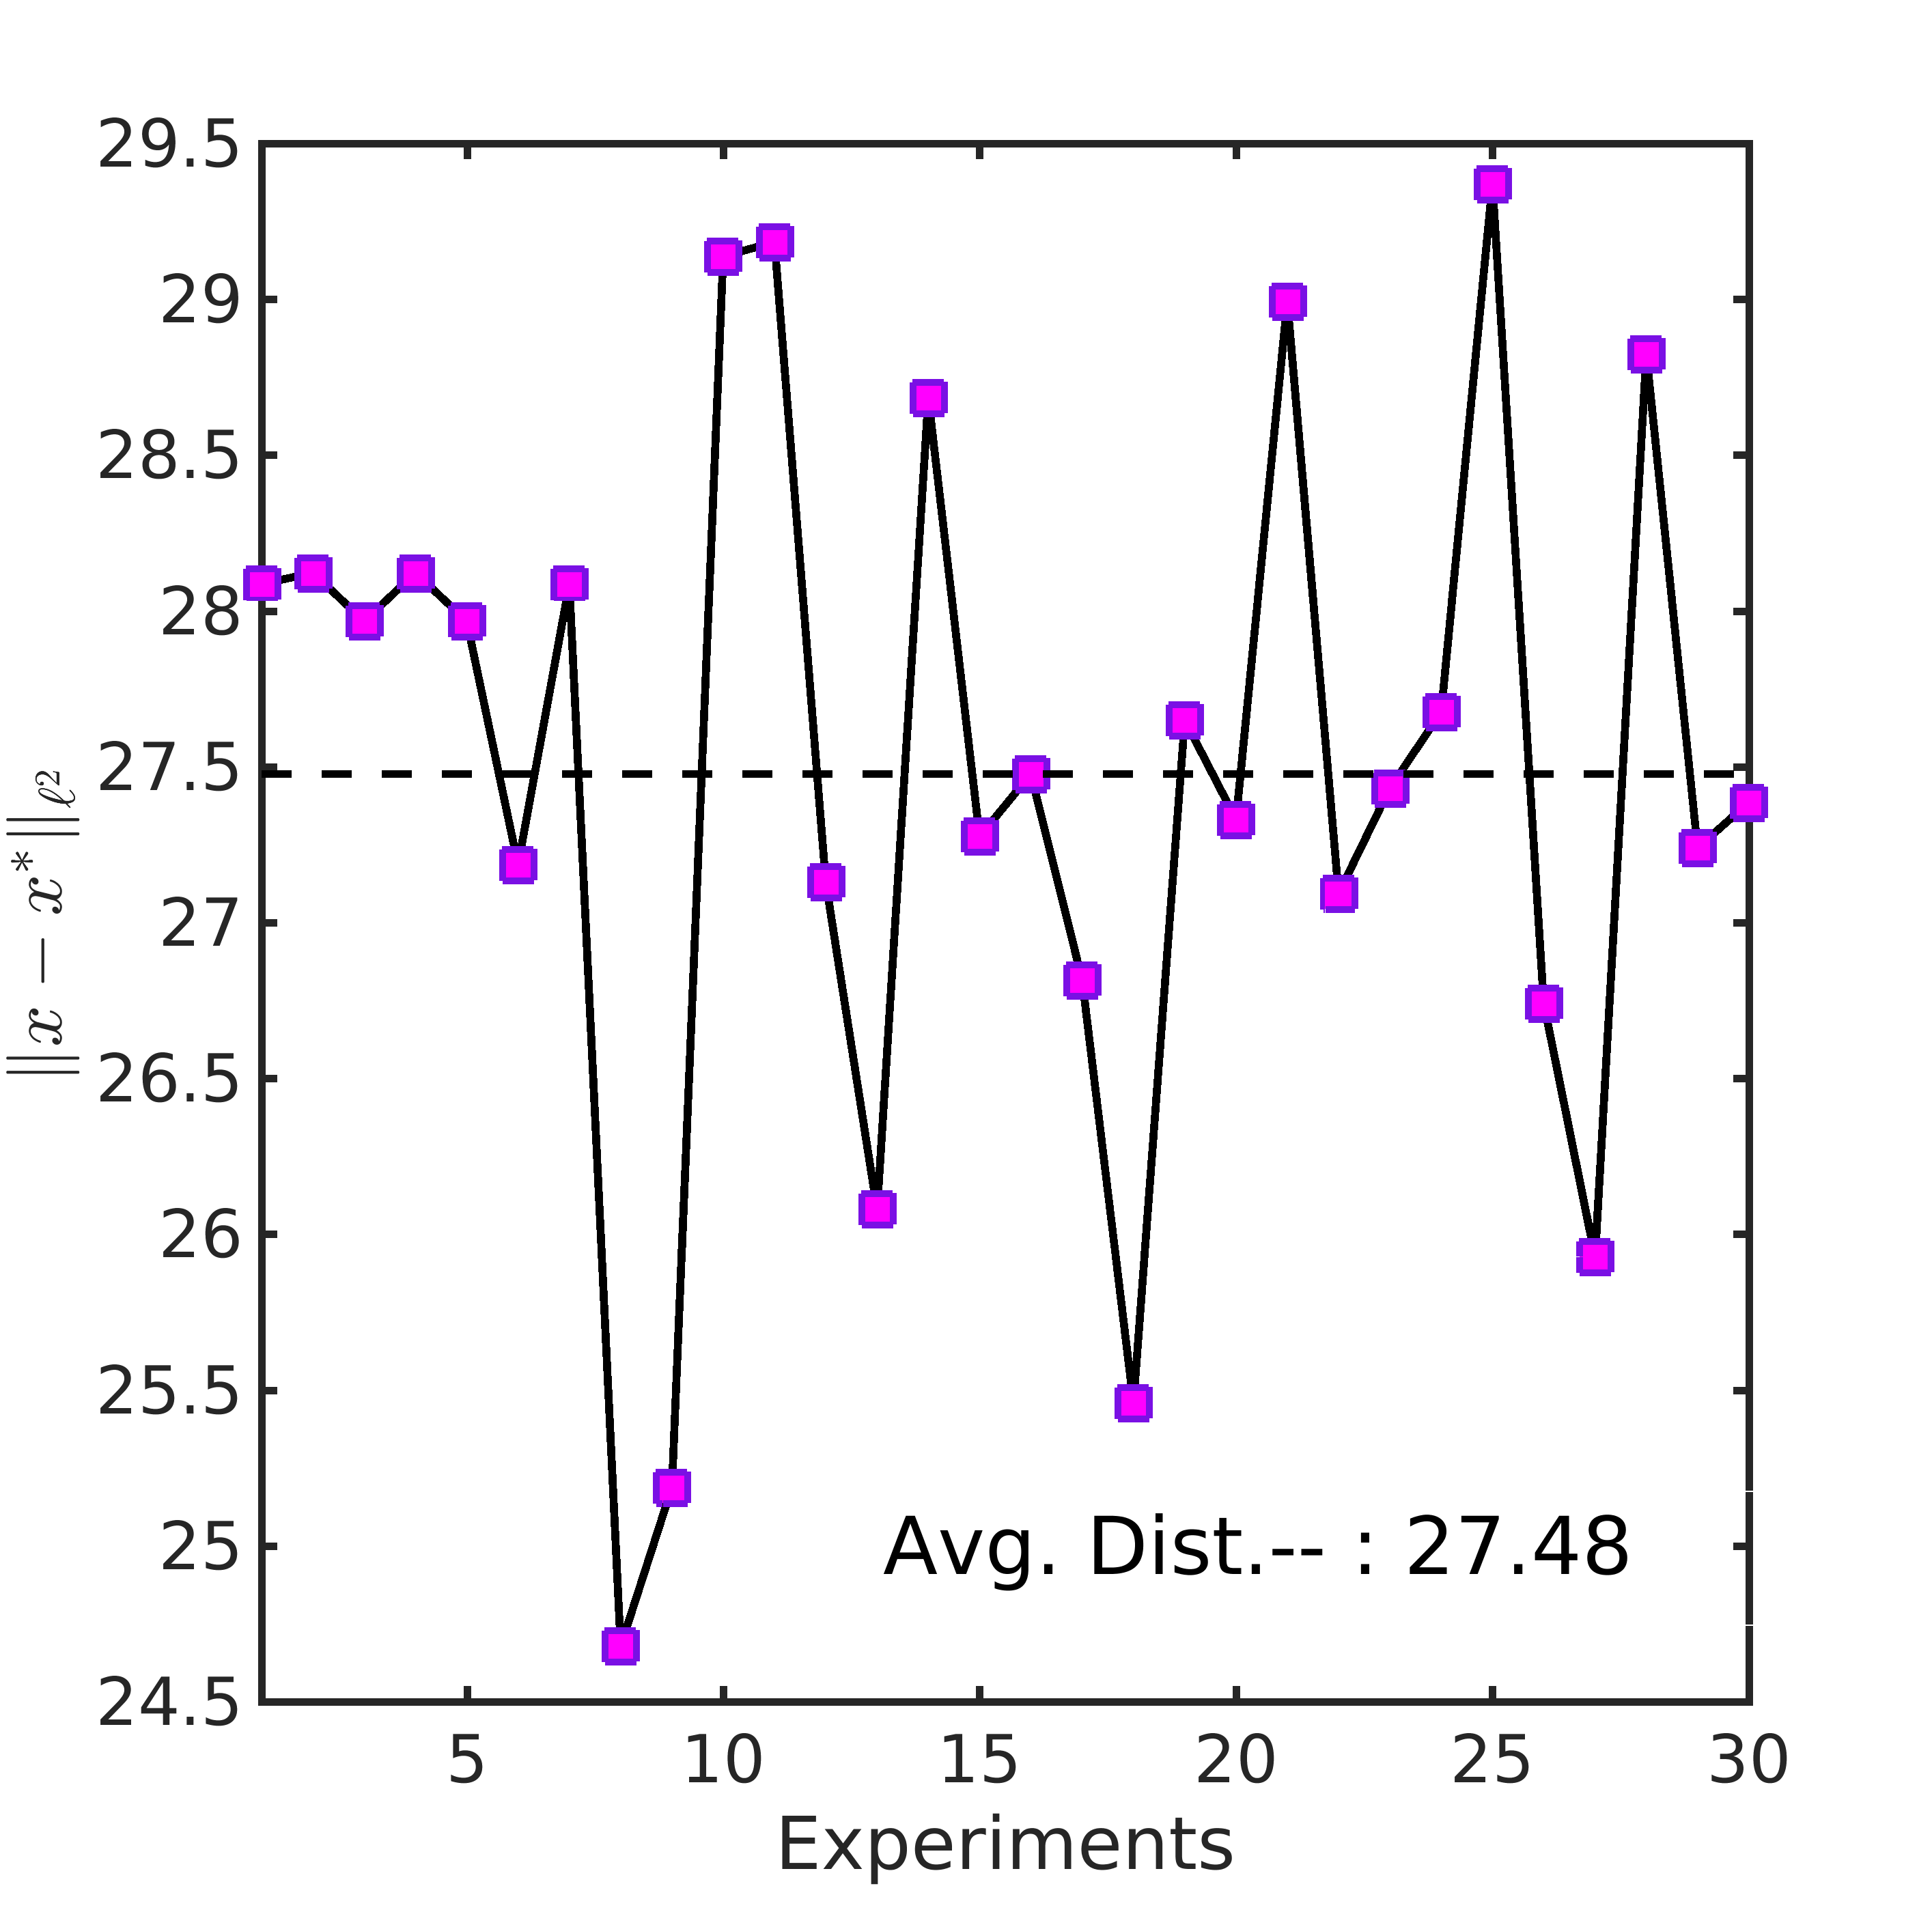
\includegraphics[scale=0.1]{./figures/ackley100Drandr0_1_dist.png}
	  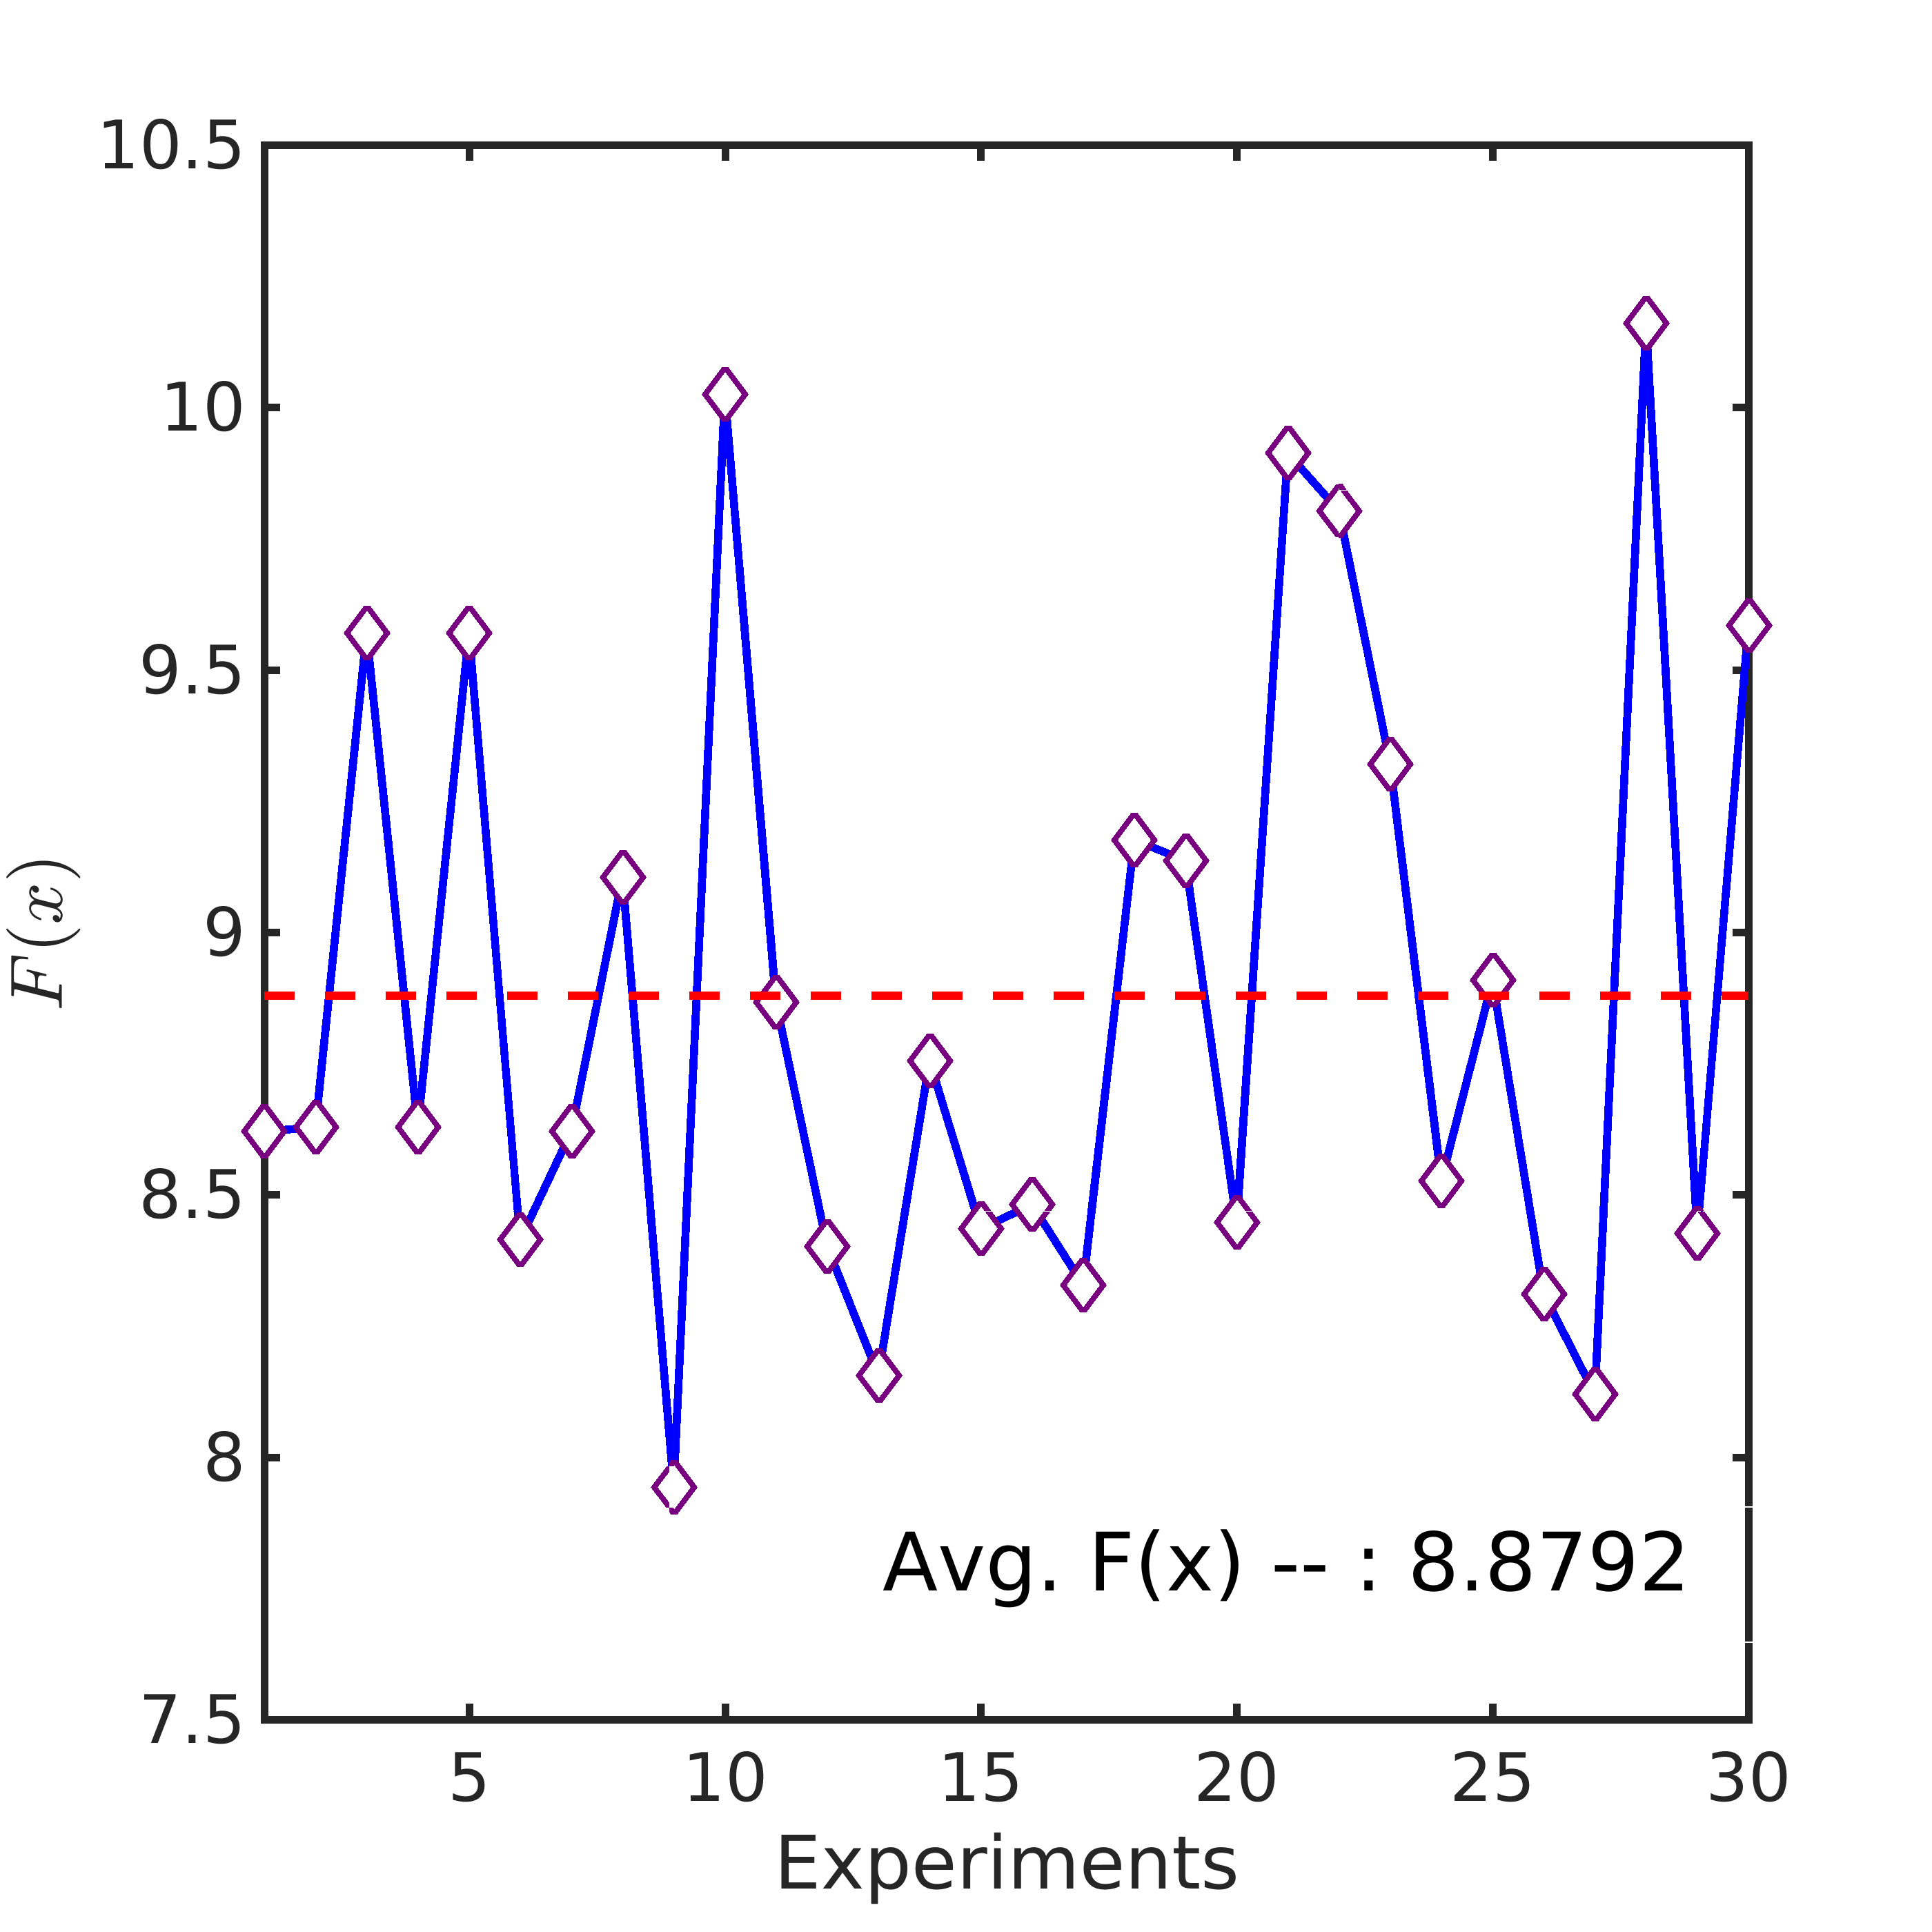
\includegraphics[scale=0.1]{./figures/ackley100Drandr0_1_val.png}
	  \vspace{-0.2cm}
	  \footnotesize{ \caption{: $\rho_0=0.1$.} }
\end{figure}
\end{columns}
\vspace{-0.6cm}
\begin{columns}[c]
	\column{6cm}
\begin{figure}[!htbp]
	\centering
	  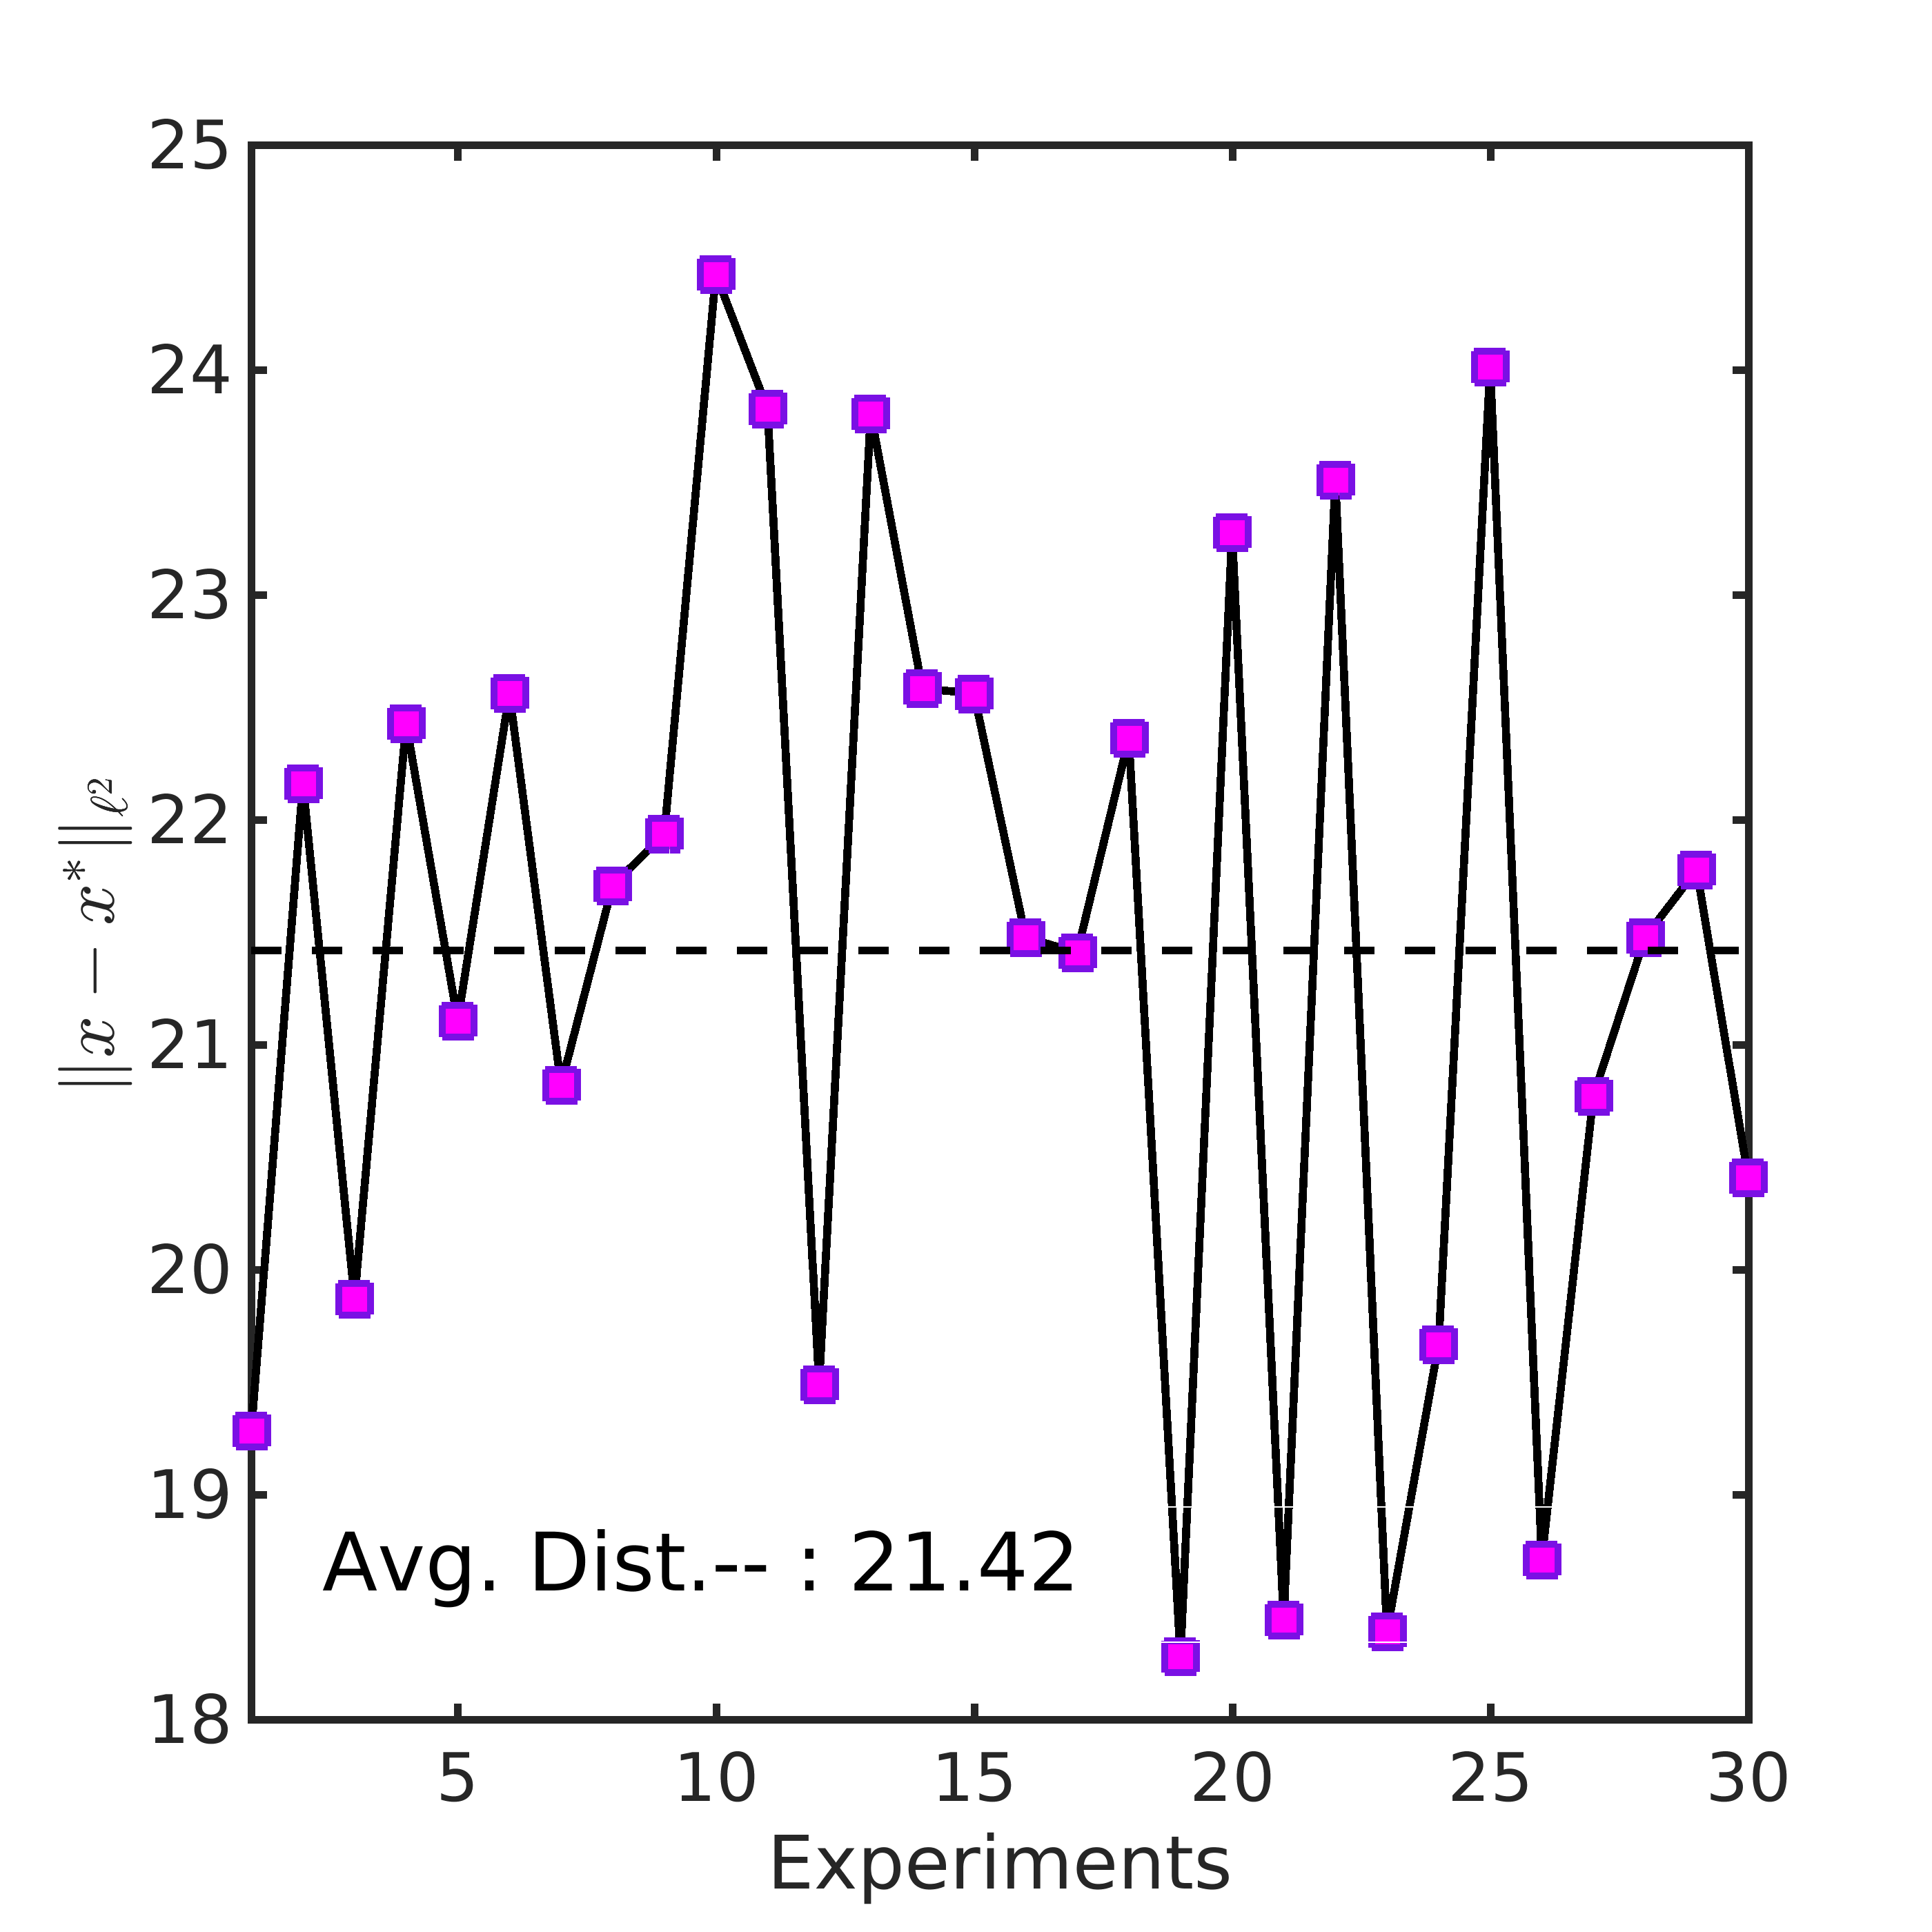
\includegraphics[scale=0.1]{./figures/ackley100Drandr0_5_dist.png}
	  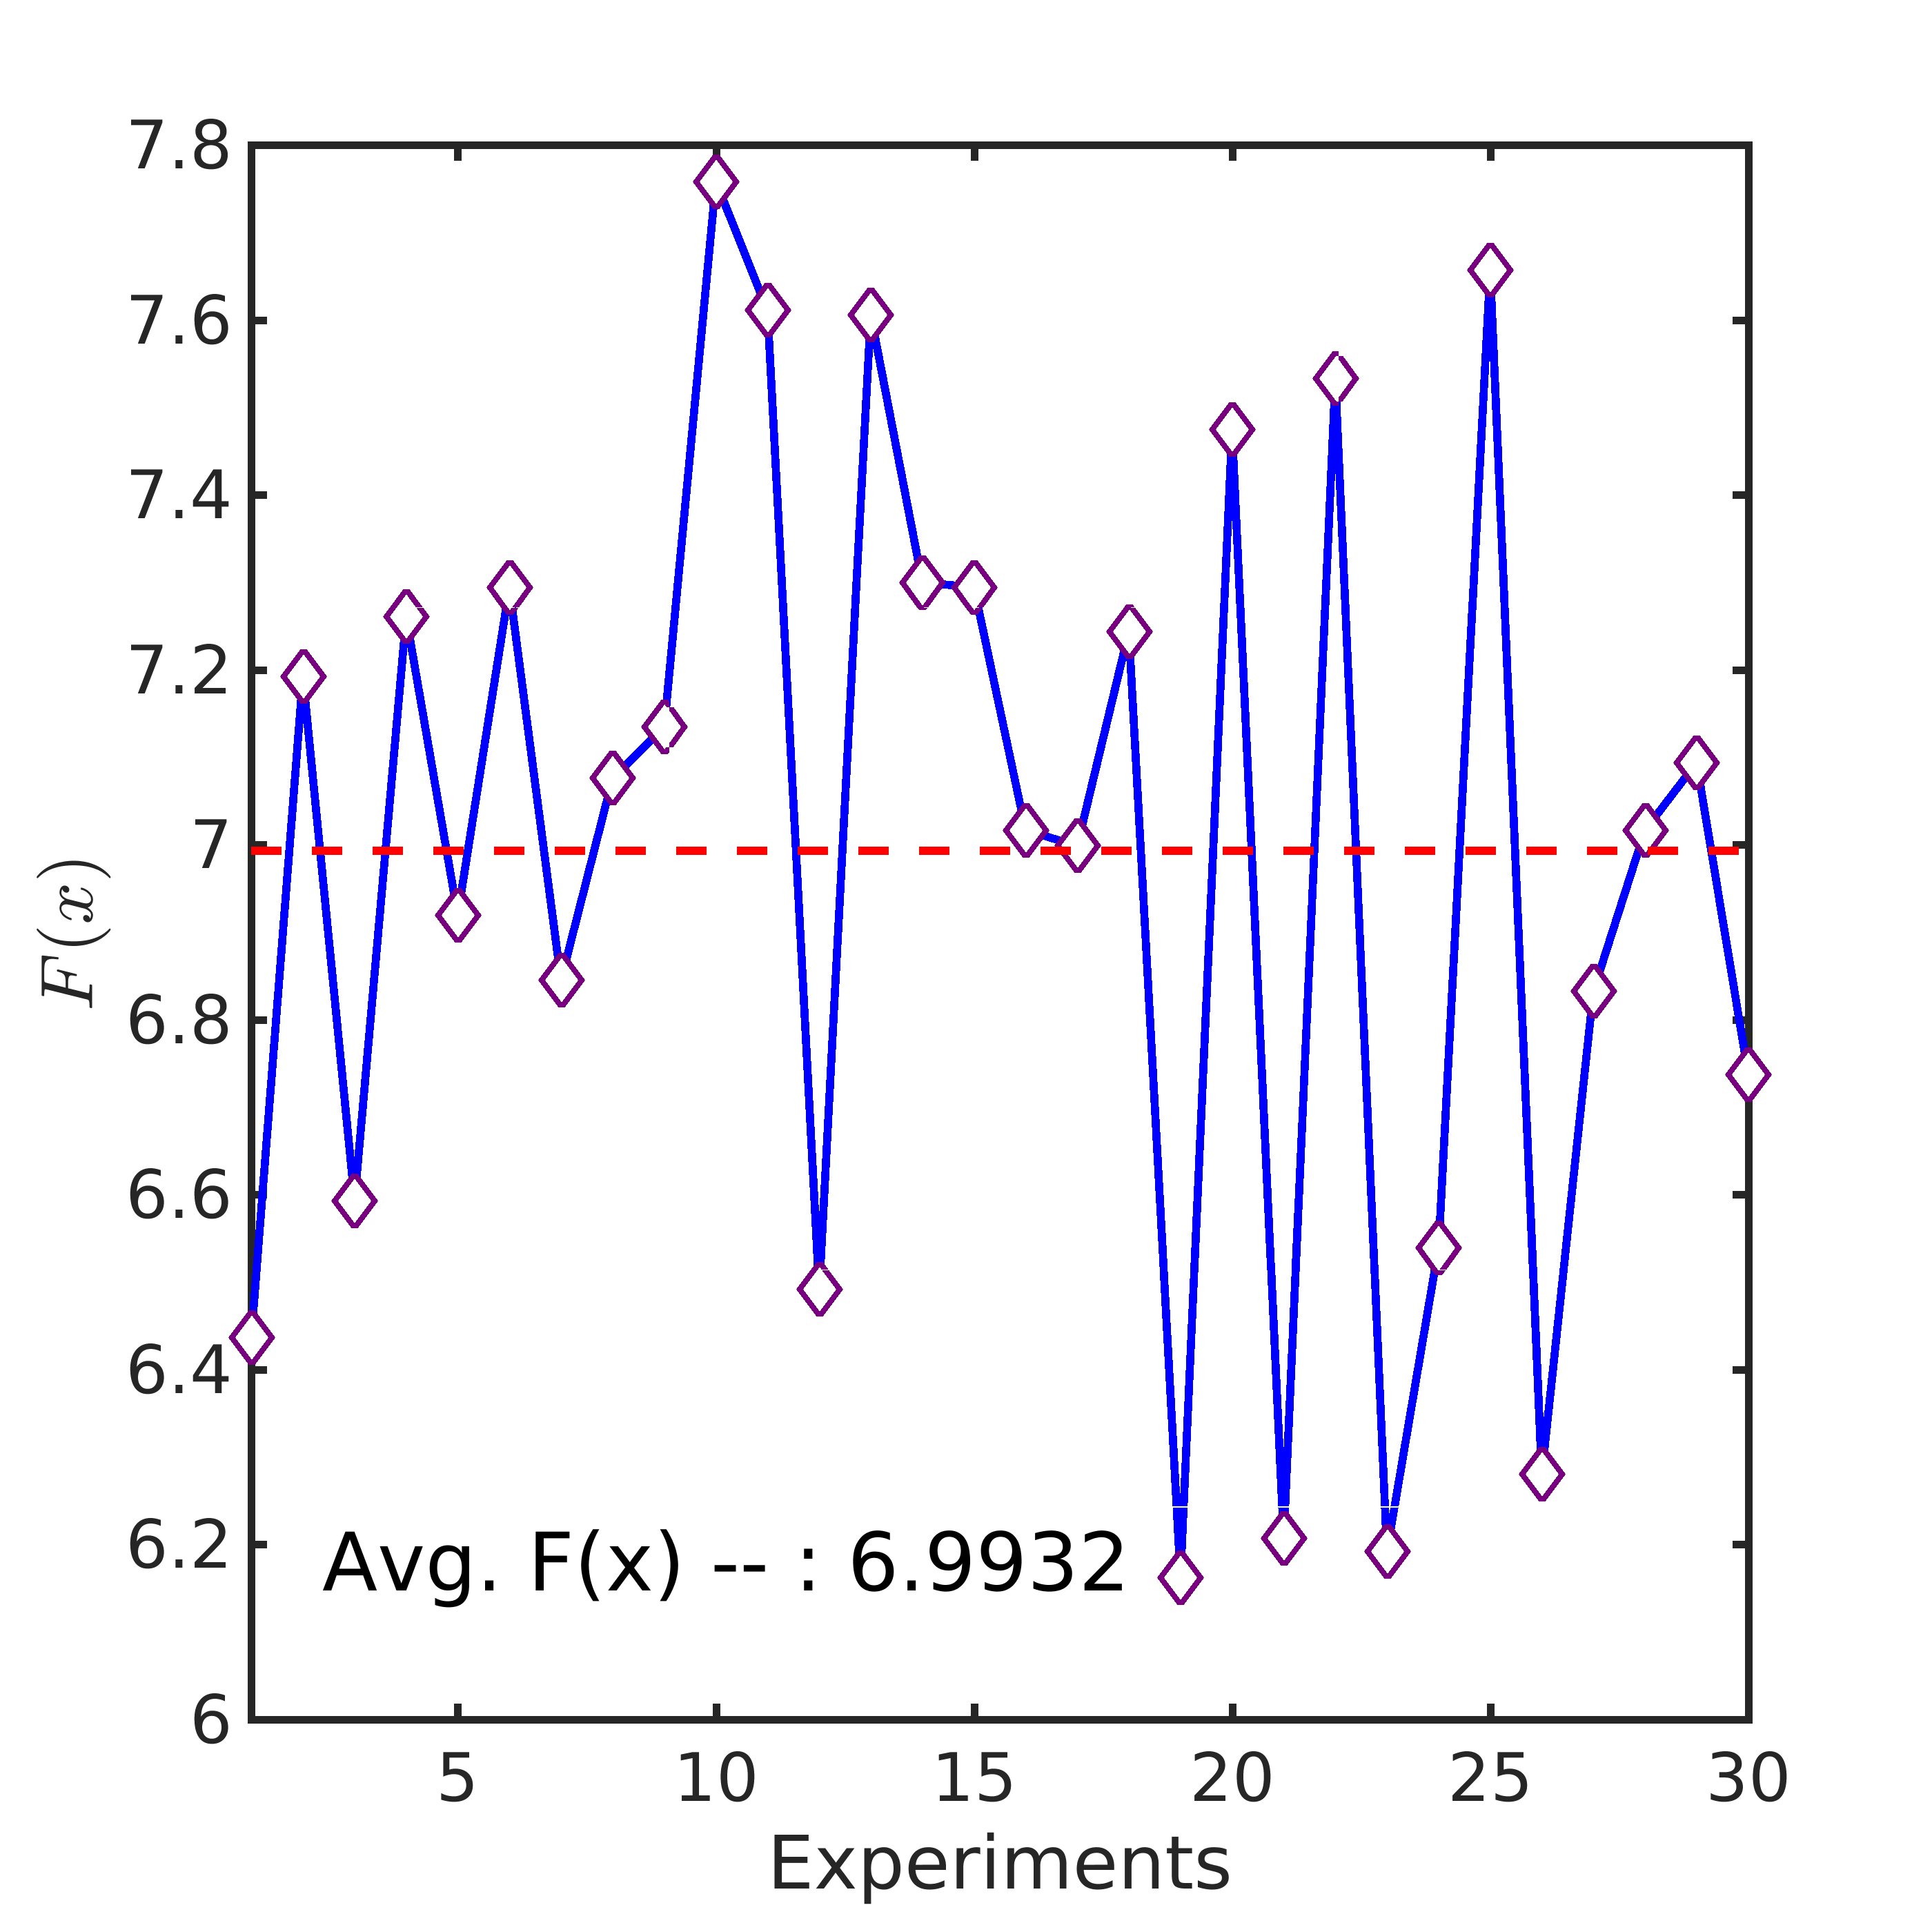
\includegraphics[scale=0.1]{./figures/ackley100Drandr0_5_val.png}
	  \vspace{-0.2cm}
	  \footnotesize{ \caption{: $\rho_0=0.5$.} }
\end{figure}
	\column{6cm}
\begin{figure}[!htbp]
	\centering
	  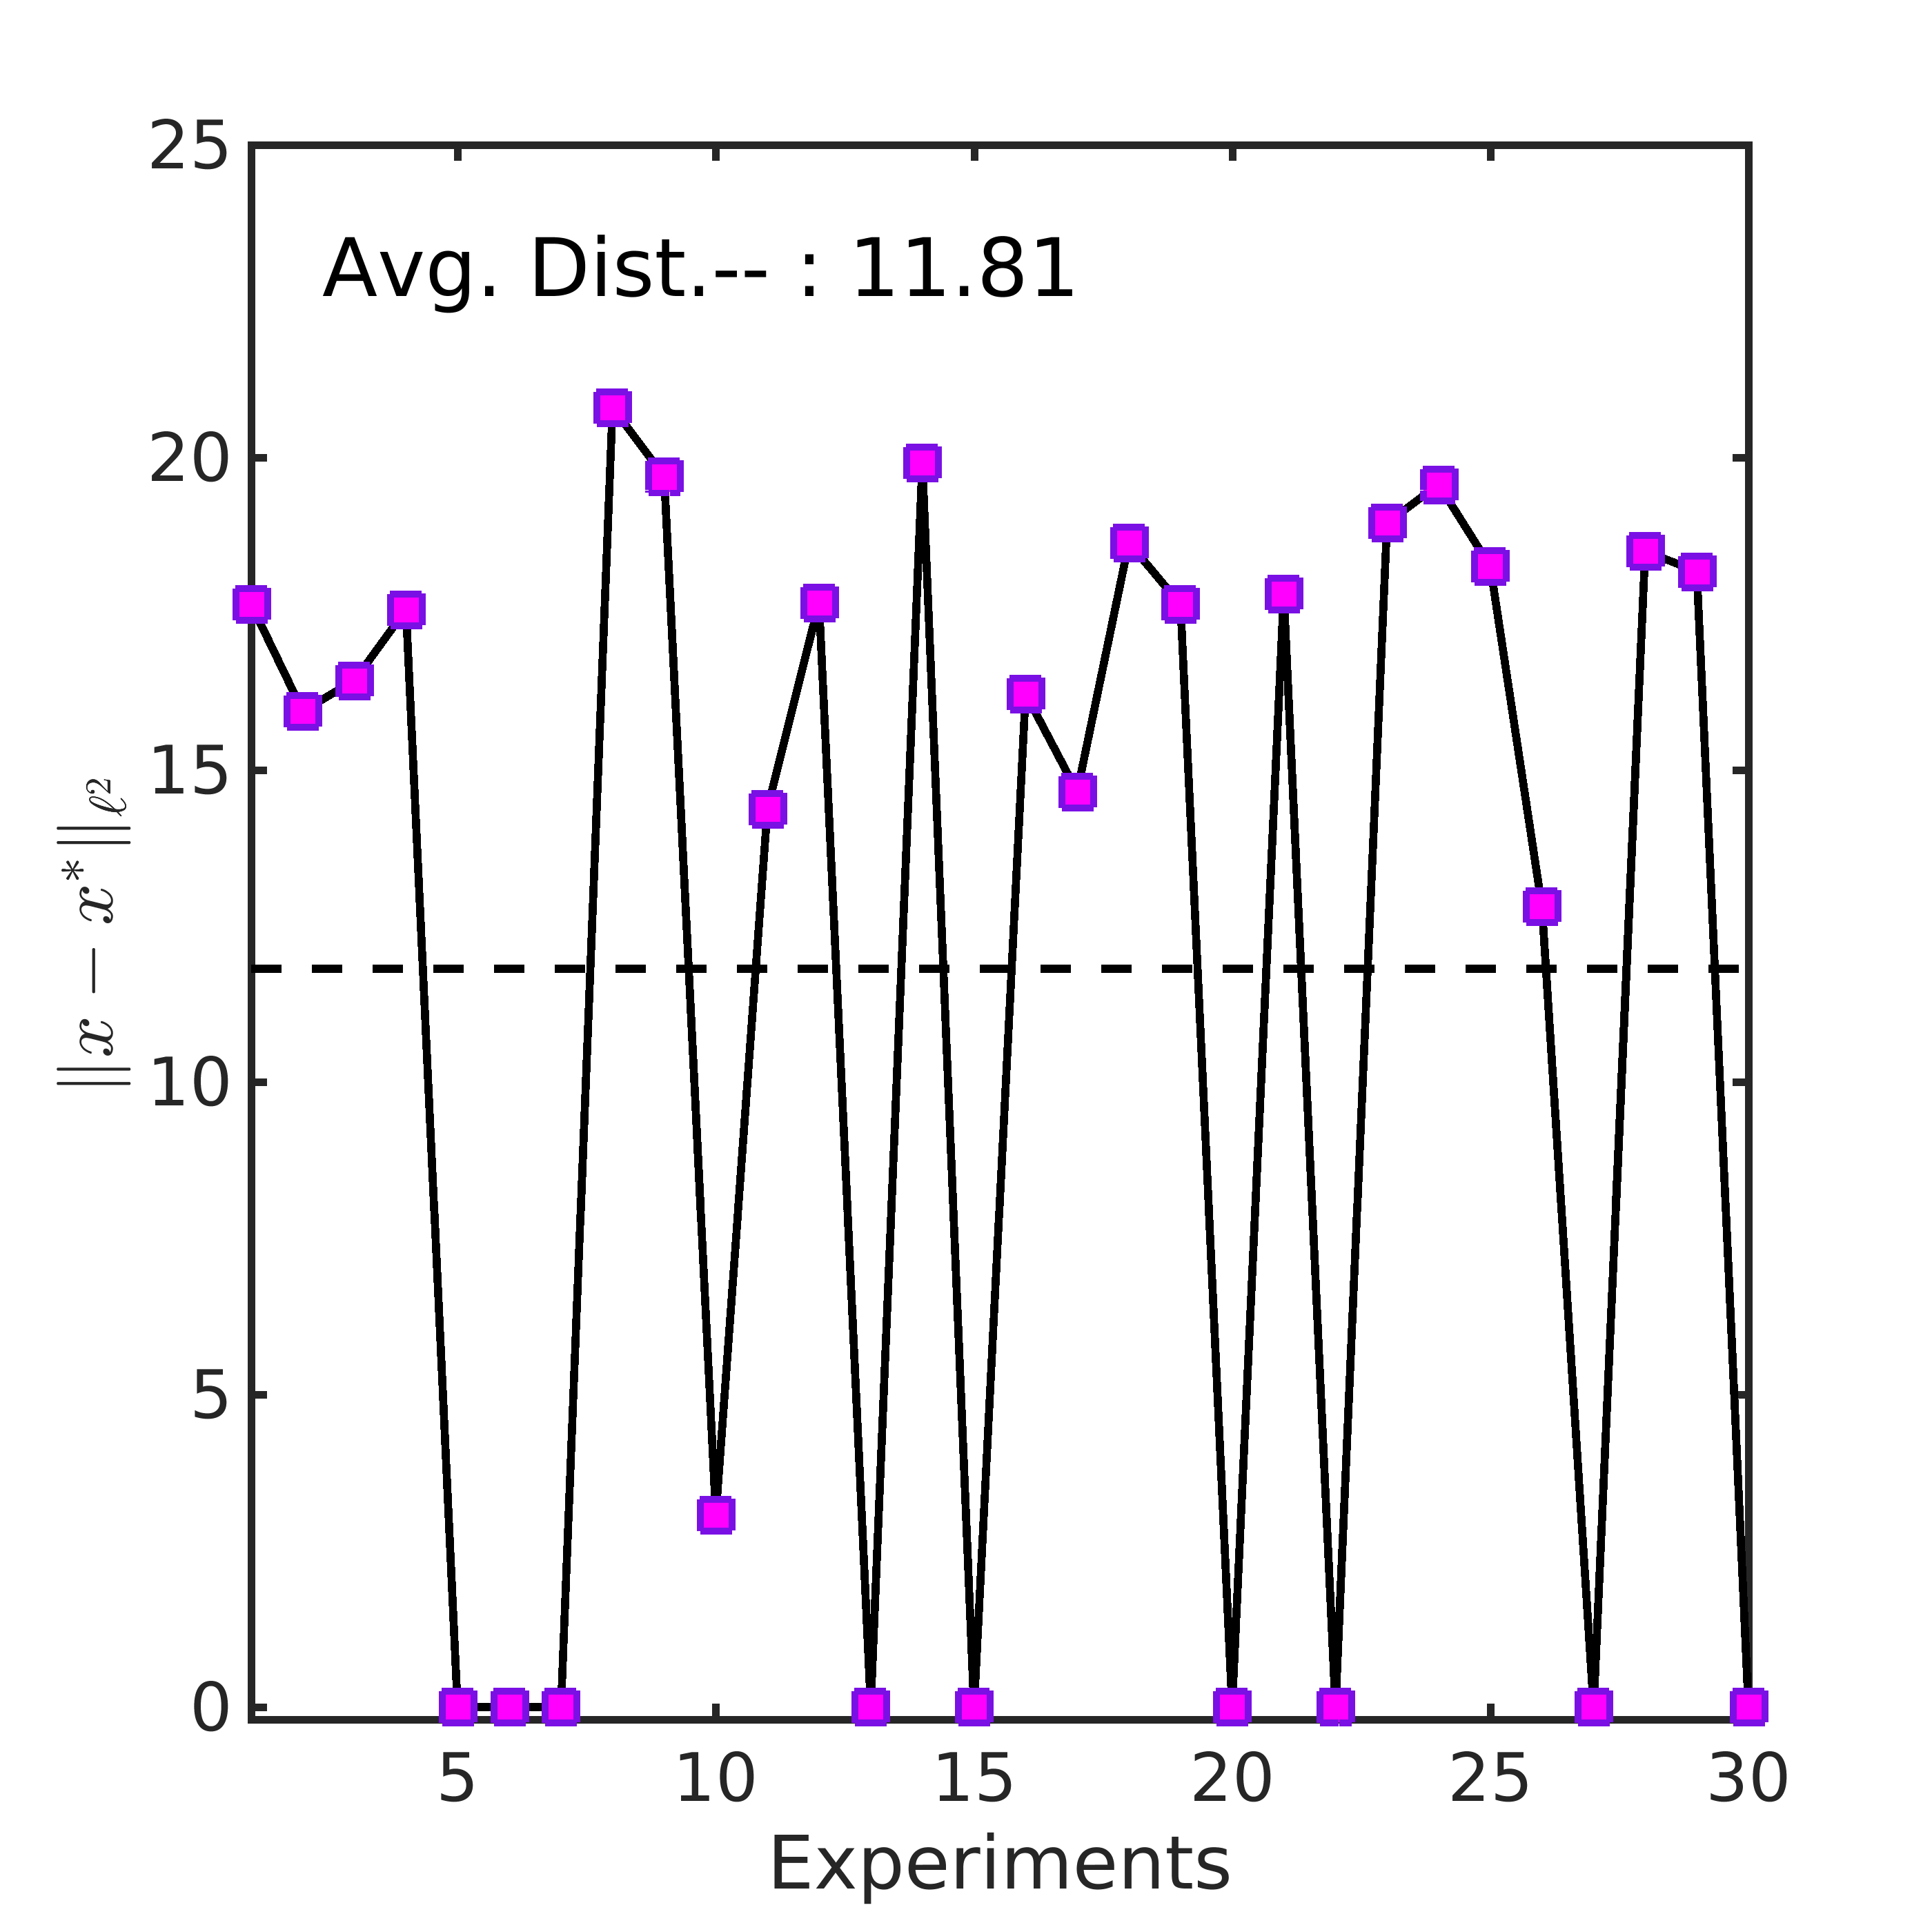
\includegraphics[scale=0.1]{./figures/ackley100Drandr0_8_dist.png}
	  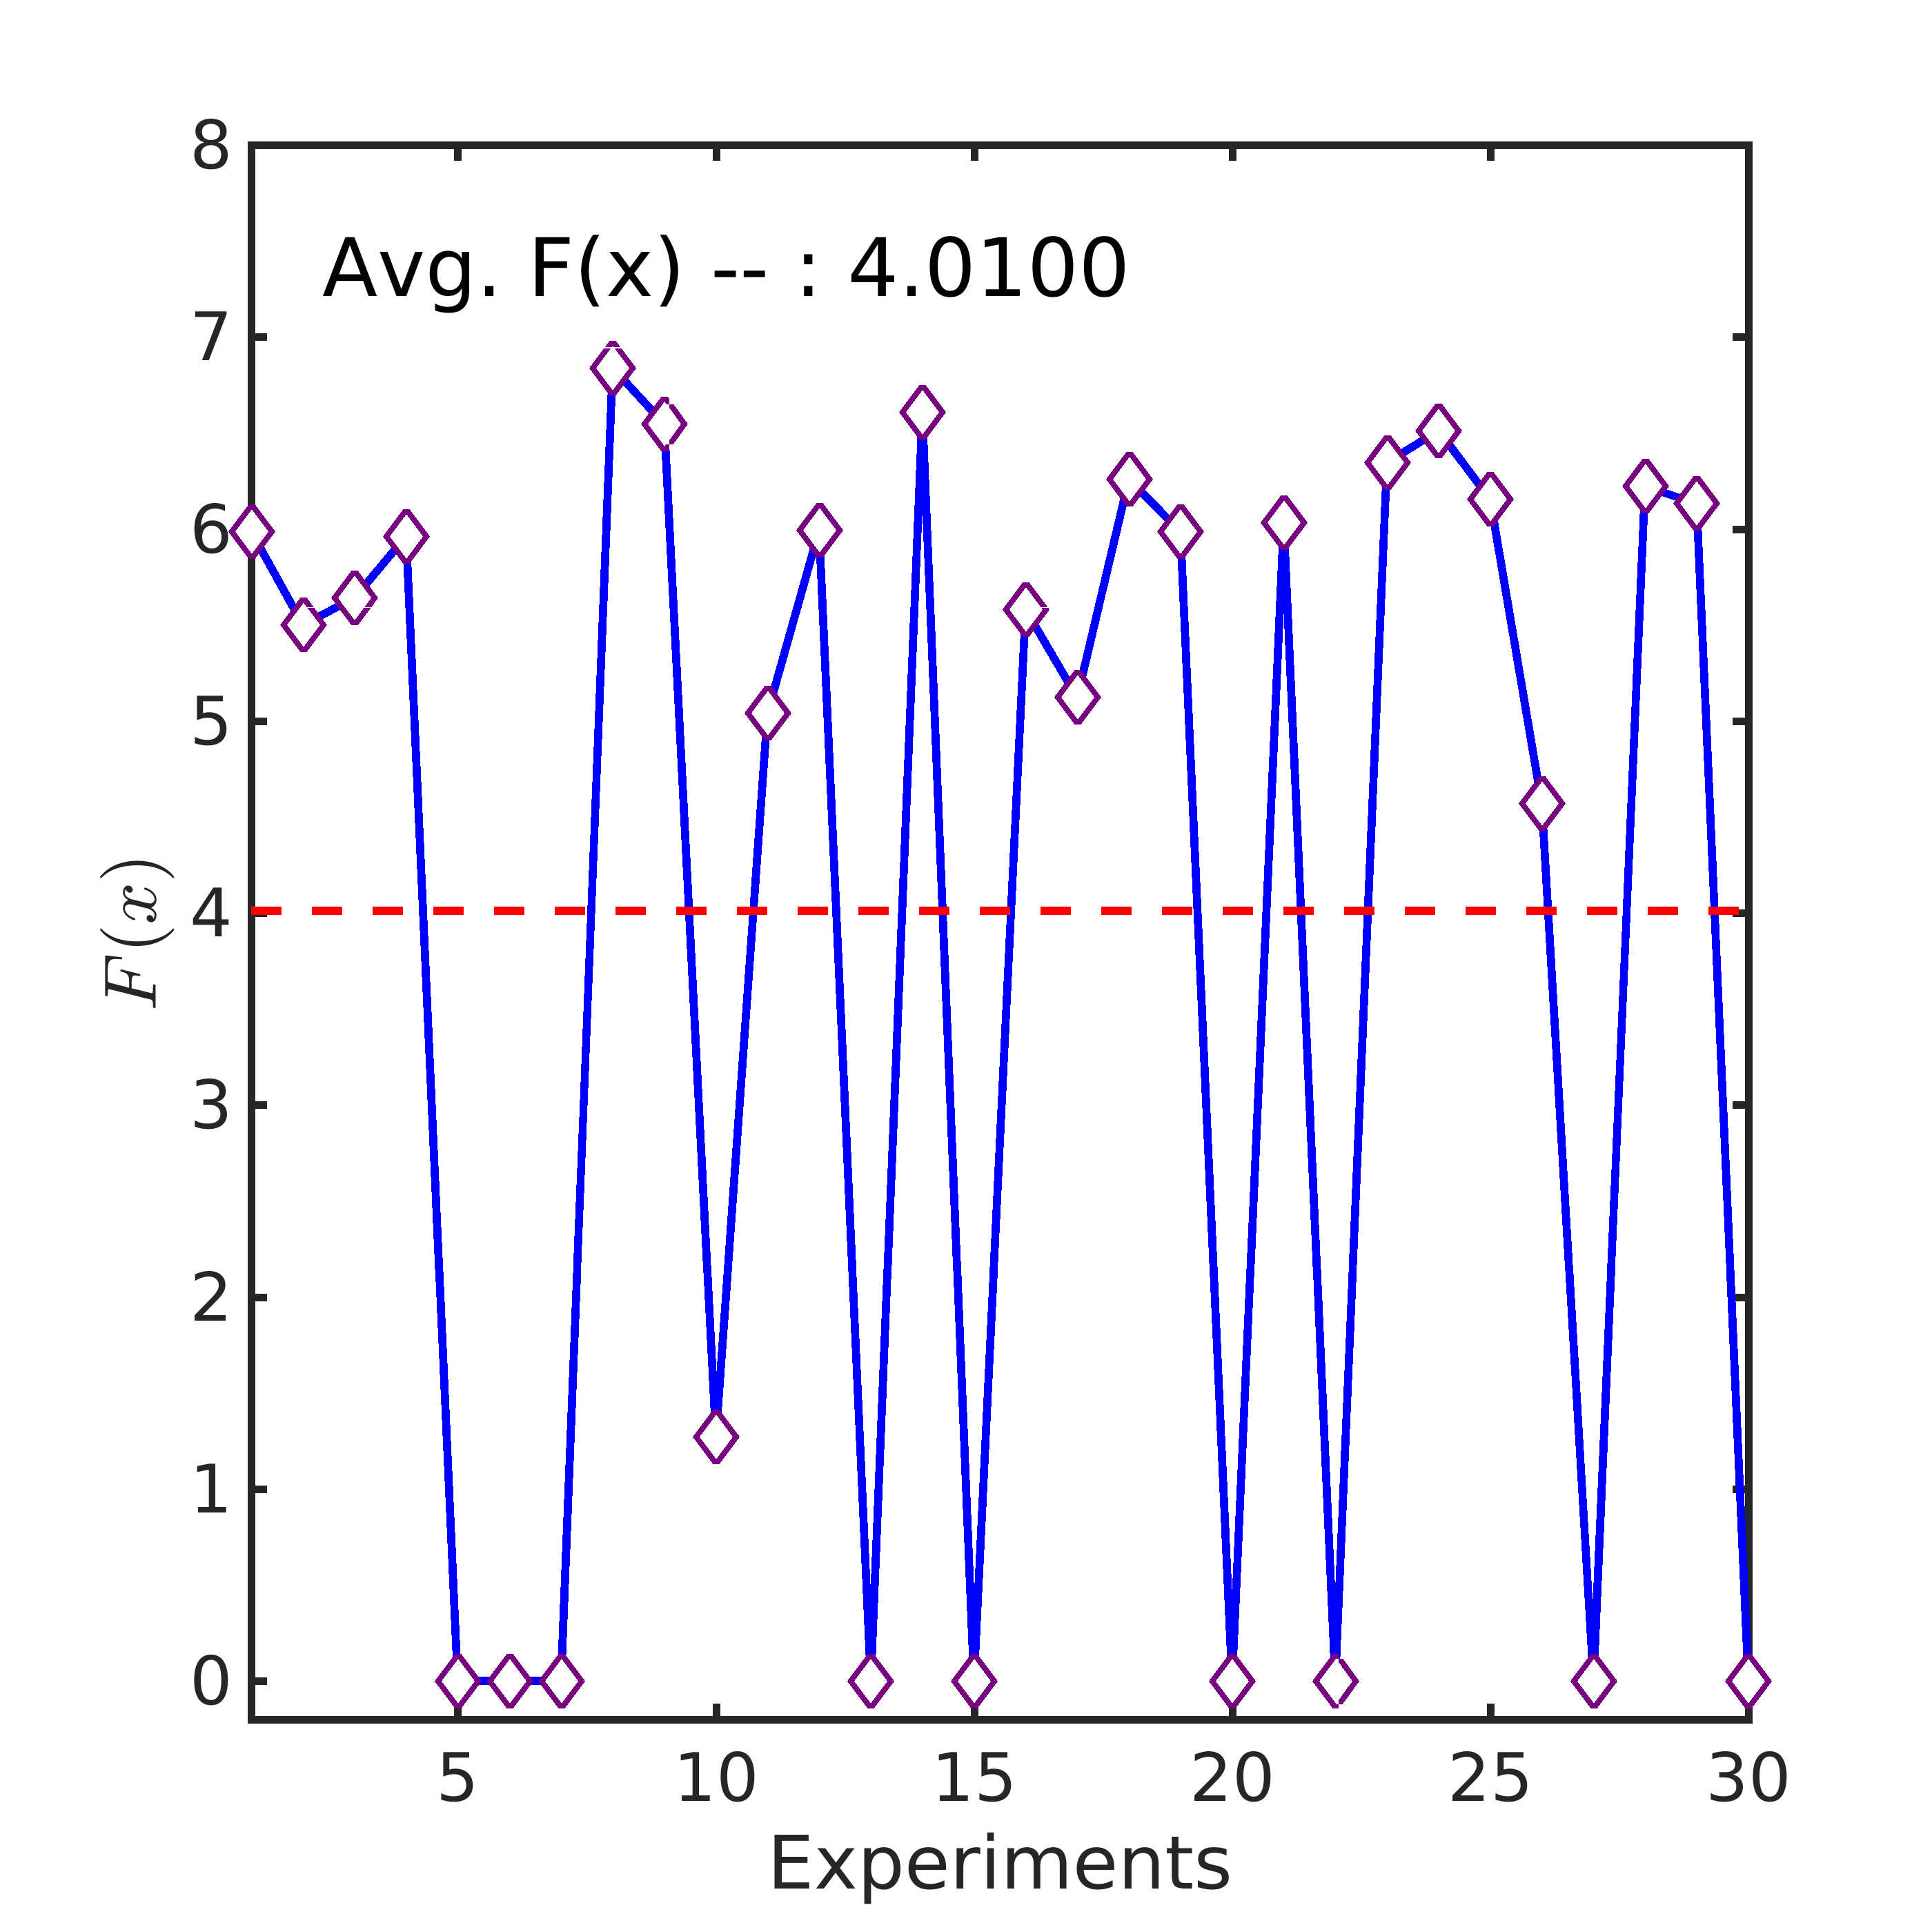
\includegraphics[scale=0.1]{./figures/ackley100Drandr0_8_val.png}
	  \vspace{-0.2cm}
	  \footnotesize{ \caption{: $\rho_0=0.8$.} }
\end{figure}
\end{columns}

\end{frame}
%%%%%%%%%%%%%%%%%%%%%%%%%%%%%%%%%%%%%%%%%%%%%%%%%%%%%%%%%%%%%%%%%%%%


%%%%%%%%%%%%%%%%%%%%%%%%%%%%%%%%%%%%%%%%%%%%%%%%%%%%%%%%%%%%%%%%%%%%
\begin{frame}{Ackley Function: 2500D}
\footnotesize{
	\begin{itemize}
		\item Apply HiCSa algorithm ($\eta=0.5$) to 2500D Ackley function with
			random initial value in  $[-10,10]^{2500}$ and $\rho_0 = 3.5$, $m_{max}=16$.
%        \item CPU time 3.7h [Intel(R) Core(TM) i7-4790, 3.60GHz]
	\end{itemize}
	}
\begin{figure}[!htbp]
	\centering
	  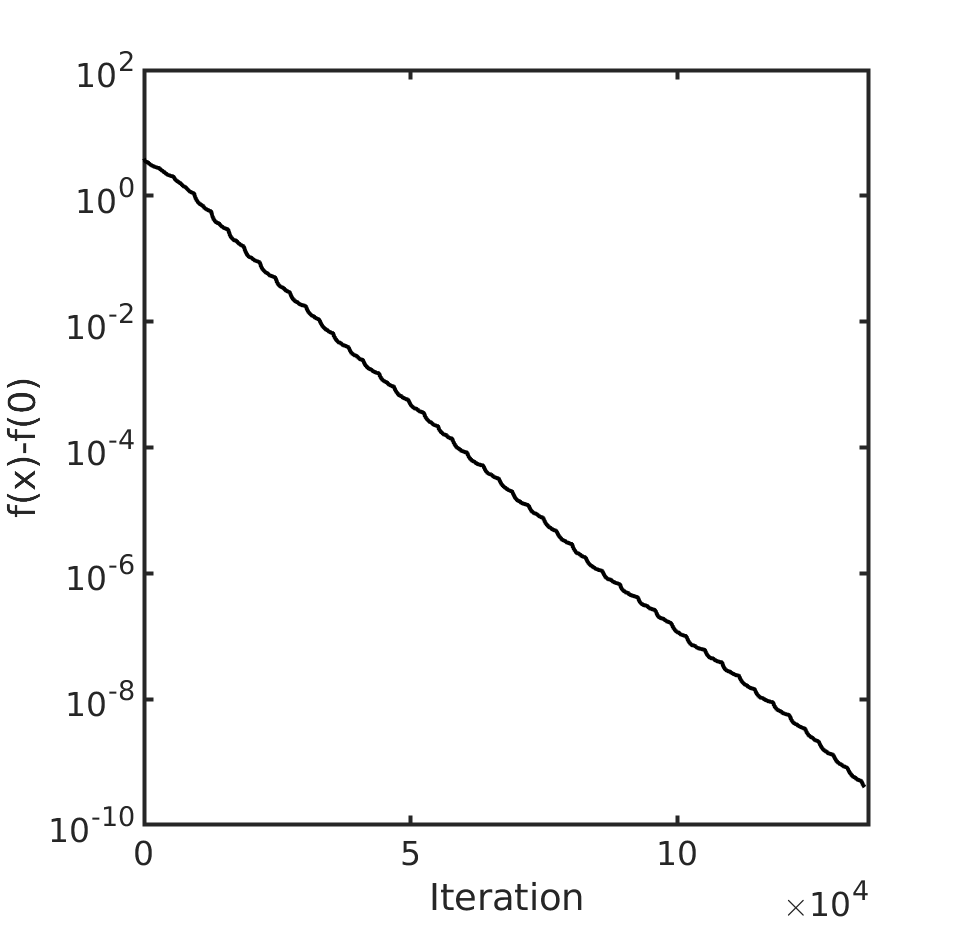
\includegraphics[scale=0.2]{./figures/ackley2500D.png}
	  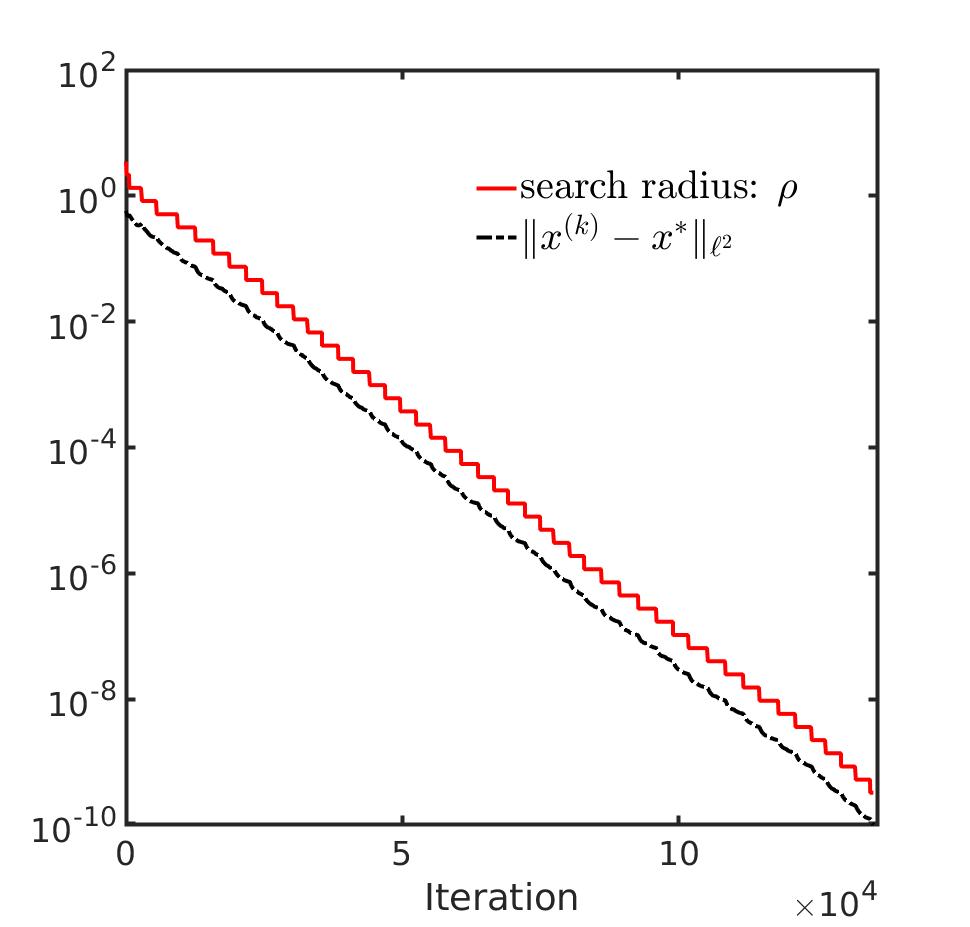
\includegraphics[scale=0.2]{./figures/ackley2500D_dist.png}
\end{figure}

%\footnotesize{
%\vspace{-0.3cm}
%\begin{table}[!htbp]
%%\caption{Iteration information}
%\begin{center}
%\begin{tabular}{|c|c|c|c|}
% \hline
%  $\rho$ &  Iter. & $\ell^2$-distance &  Fun. Val.
% \\\hline
%3.5 &  \makecell{ 5415 } & \makecell{ 1.8854368262e+02 \\ $\downarrow$ \\ 4.3980512458e+01  }
% & \makecell{  1.2310134936e+01 \\ $\downarrow$ \\  4.7600200861e+00}
% \\\hline
%1.75 &  \makecell{ 5064 } & \makecell{ $\downarrow$ \\  2.4909250731e+01 }
% & \makecell{   $\downarrow$ \\ 3.3115891477e+00 }
% \\\hline
%8.75e-01&  \makecell{ 4099 } & \makecell{ $\downarrow$ \\  1.0893125123e+01 }
% & \makecell{   $\downarrow$ \\ 2.0271413426e+00 }
% \\\hline
%4.375e-01&  \makecell{ 4869 } & \makecell{ $\downarrow$ \\  5.1289809138e+00 }
% & \makecell{   $\downarrow$ \\  8.8082043719e-01}
% \\\hline
%2.1875e-01&  \makecell{ 3269 } & \makecell{ $\downarrow$ \\ 2.5698591962e+00 }
% & \makecell{   $\downarrow$ \\ 3.4009221628e-01 }
% \\\hline
% $\downarrow$ & $\downarrow$ & $\downarrow$  & $\downarrow$
% \\\hline
%1.335144e-05 & 3340  & 1.5546421188e-04 & 1.2437651812e-05
% \\\hline
%\end{tabular}
%\end{center}
%\end{table}
%}
\end{frame}
%%%%%%%%%%%%%%%%%%%%%%%%%%%%%%%%%%%%%%%%%%%%%%%%%%%%%%%%%%%%%%%%%%%%

\subsection{Woods Function}
%%%%%%%%%%%%%%%%%%%%%%%%%%%%%%%%%%%%%%%%%%%%%%%%%%%%%%%%%%%%%%%%%%%%
\begin{frame}{Woods Function (CUTE)}

\footnotesize{
\begin{equation*}
	\begin{aligned}
		F(x) = \sum^{n/4}_{i=1} \Big[100(x_{4i-2}-x^2_{4i-3})^2 +
		(1-x_{4i-3})^2 + 90(x_{4i}-x_{4i-1})^2 +
		\\
		(1-x_{4i-1})^2 + 10(x_{4i-2}+x_{4i}-2)^2 +
		0.1(x_{4i-2}-x_{4i})^2
		\Big].
	\end{aligned}
\end{equation*}
}
\footnotesize{
\noindent The global minimizer is $(1,1,\dots,1)$ with $f=0$.
The initial value $x_j^{(0)}=-3.0$ if
$j$ is even, and  $x_j^{(0)}=-1.0$ if $j$ odd.
%The choices of $n$ are $4$, $20$, $80$, $320$, $1280$, $2000$.
We apply HiCS algorithm to 320D Woods functions with
$\rho_0 = 5$ and $m_{\max}=8$.
}
%
%\begin{table}[!htbp]
%\begin{center}
%\begin{tabular}{|c|c|c|c|c|}
% \hline
%n & Iterations & $\ell^2$-distance & $F(x)$ & \# $F$
%\\ \hline
%4 & 8 & 3.2768793351 & 6.9073368732e+02 & 100
%\\ \hline
%20 & 23 & 1.0972975755e+01 & 4.0331497607e+03 & 609
%\\ \hline
%80 & 111 & 2.0269797302e+01 & 1.9462281448e+04 & 10125
%\\ \hline
%320 & 586 &3.4206914228e+01 & 4.8860690790e+04 & 192279
%\\ \hline
%400 & &&&
%\\ \hline
%480 & &&&
%\\ \hline
%1280 & 2431 & 7.1988770199e+01 & 2.1053246815e+05 & 3198657
%%\\ \hline
%%2000 &  & & &
%\\ \hline
%\end{tabular}
%\end{center}
%\end{table}
\begin{figure}[!htbp]
	\centering
	  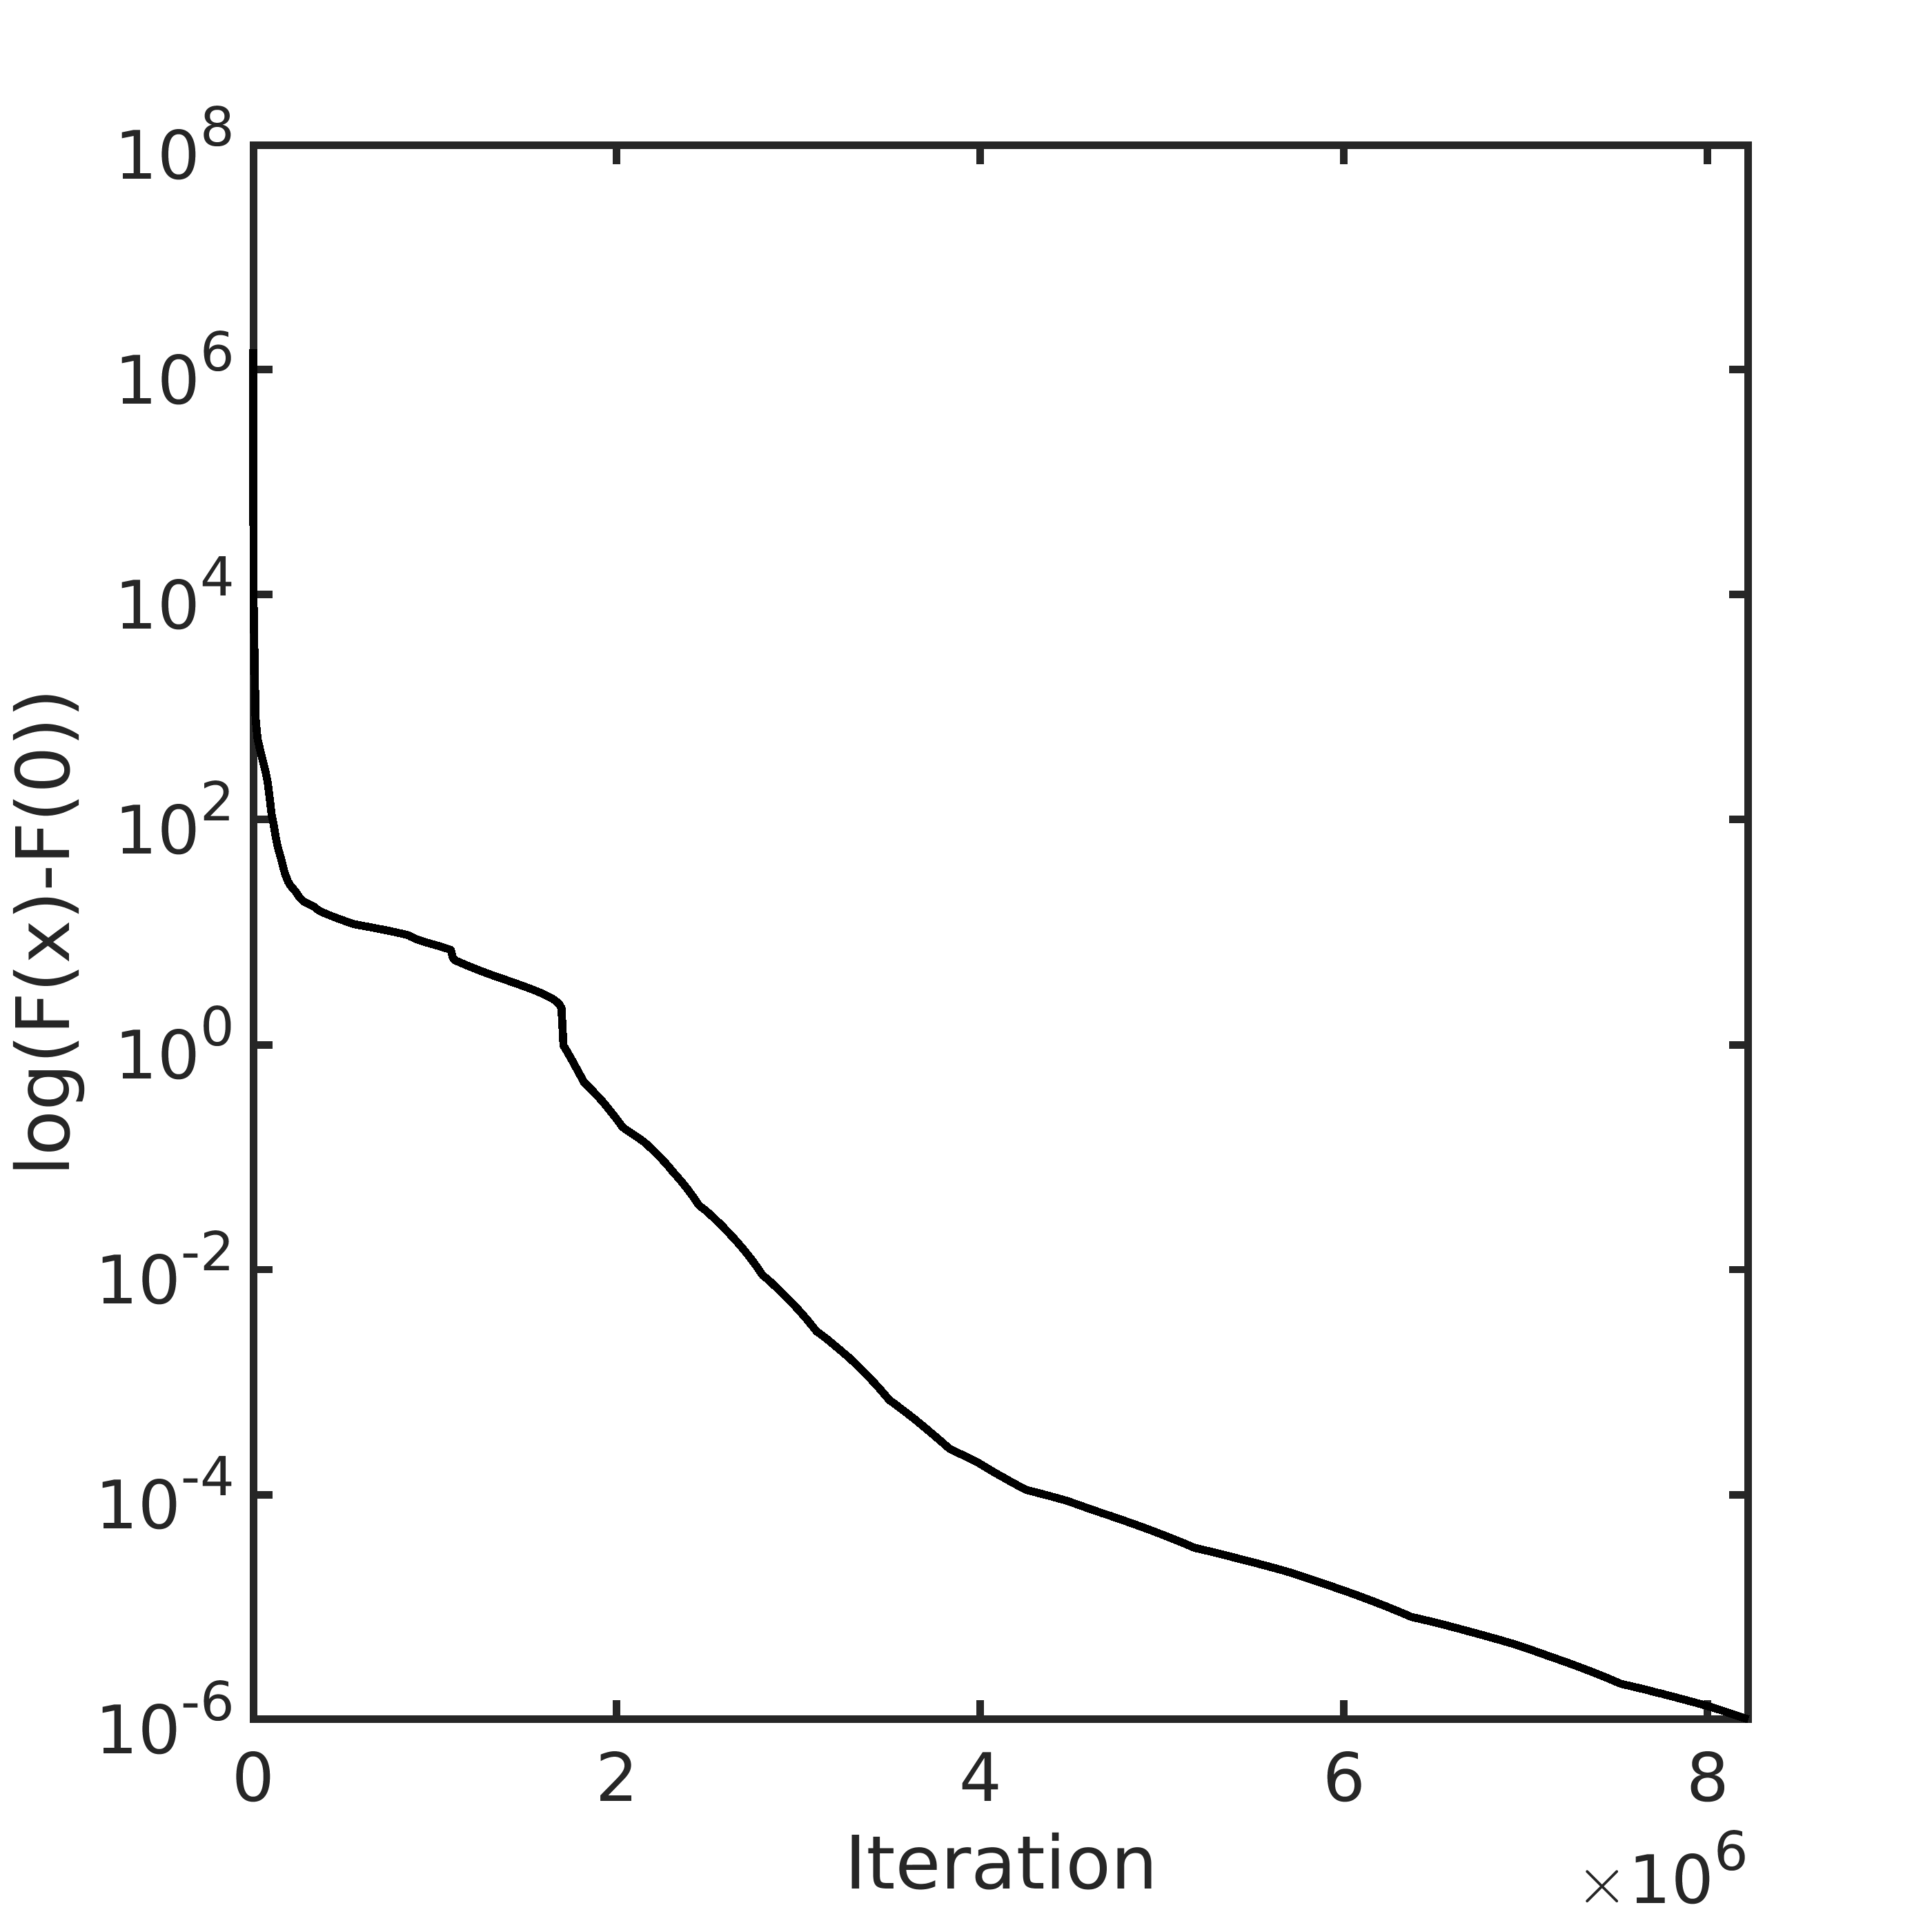
\includegraphics[scale=0.15]{./figures/woods320D.png}
	  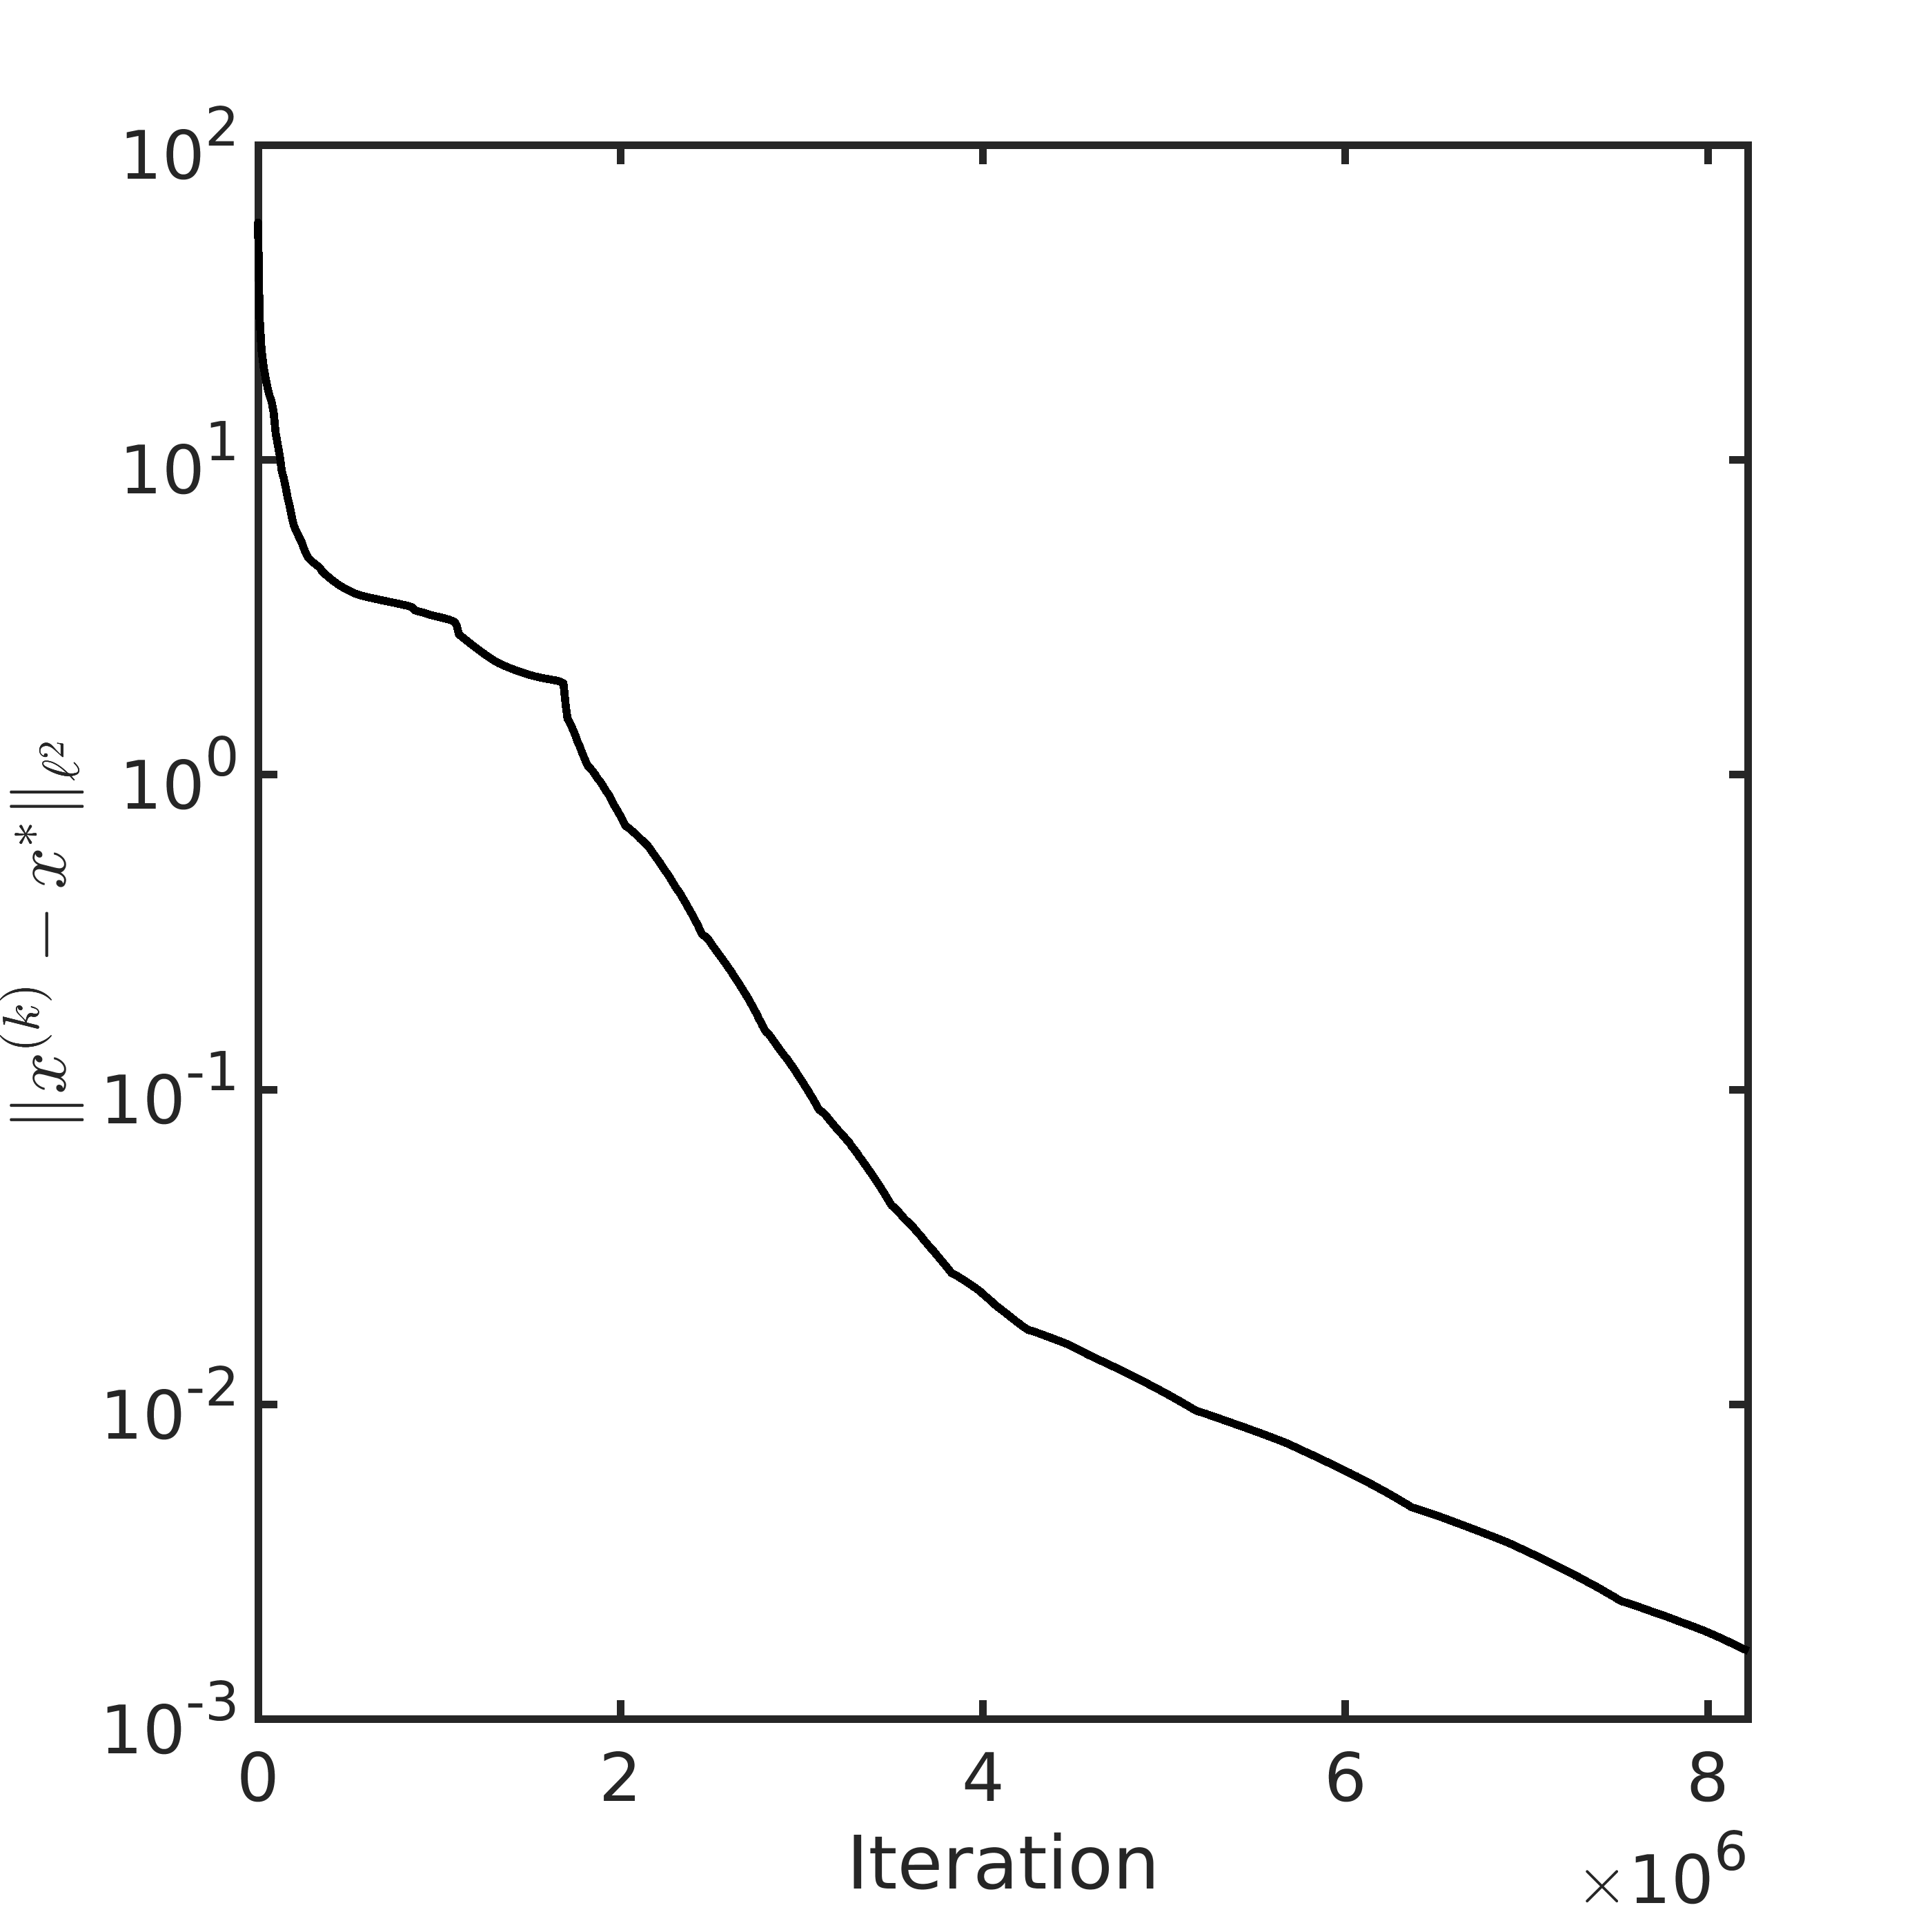
\includegraphics[scale=0.15]{./figures/woods320D_dist.png}
\end{figure}
\end{frame}
%%%%%%%%%%%%%%%%%%%%%%%%%%%%%%%%%%%%%%%%%%%%%%%%%%%%%%%%%%%%%%%%%%%%


%%%%%%%%%%%%%%%%%%%%%%%%%%%%%%%%%%%%%%%%%%%%%%%%%%%%%%%%%%%%%%%%%%%%%
%\begin{frame}{80D Woods Function: HiCSa}
%
%\footnotesize{
%}
%%The global minimizer is $(1,1,\dots,1)$ with $f=0$.
%%The initial value $x_j^{(0)}=-3.0$ if
%%$j$ is even, and  $x_j^{(0)}=-1.0$ if $j$ odd.
%%The choices of $n$ are $4$, $20$, $80$, $320$, $1280$, $2000$.
%We can further apply HiCSa approach ($\eta=0.5$) to approximating the
%minimizer of Woods function based on the above convergent results.
%Here we take $n=80$ as an example to demonstrate the iteration procedure.
%
%
%\begin{table}[!htbp]
%\begin{center}
%\begin{tabular}{|c|c|c|c|}
% \hline
%  $\rho$ &  Iter. & $\ell^2$-distance & $F(x)$
% \\\hline
%5.0 &  \makecell{ 111 } & 2.0269797302e+01 & 1.9462281448e+04
% \\\hline
%2.5 &  \makecell{ 21 } & 2.1446697698e+01 & 1.7213410433e+04
% \\\hline
%1.25&  \makecell{ 38 } & 2.3007762412e+01 & 1.4027762445e+04
% \\\hline
%0.625& \makecell{ 49 } & 2.1442322133e+01 & 9.2058823364e+03
% \\\hline
%0.3125&  \makecell{ 558 } & 1.8950544937e+01 & 2.3646230729e+03
% \\\hline
%0.15625&  \makecell{ 634 } & 1.6684359010e+01 & 1.2099516621e+03
% \\\hline
%0.078125&  \makecell{ 2502 } & 1.2212940331e+01 & 2.9382990538e+02
% \\\hline
% $\downarrow$ & $\downarrow$ & $\downarrow$  & $\downarrow$
% \\\hline
%1.907349e-05 & 114180  & 4.4027298178e-02 & 7.0921802110e-04
% \\\hline
%\end{tabular}
%\\
%\vspace{0.3cm}
%It costs $48665367$ function evaluations.
%\end{center}
%\end{table}
%
%\end{frame}
%%%%%%%%%%%%%%%%%%%%%%%%%%%%%%%%%%%%%%%%%%%%%%%%%%%%%%%%%%%%%%%%%%%%%


%%%%%%%%%%%%%%%%%%%%%%%%%%%%%%%%%%%%%%%%%%%%%%%%%%%%%%%%%%%%%%%%%%%%%
%\begin{frame}{Sphere Function}
%
%\footnotesize{
%\begin{align*}
%    f(x) = \sum_{i=1}^n x_i^2
%\end{align*}
%The Sphere function has $n$ local minima except for the
%global one $x=(0,0,\dots,0)$ with $f=0$.
%It is continuous, convex and unimodal.
%}
%
%\end{frame}
%%%%%%%%%%%%%%%%%%%%%%%%%%%%%%%%%%%%%%%%%%%%%%%%%%%%%%%%%%%%%%%%%%%%%

\subsection{ARWHEAD Function}
%%%%%%%%%%%%%%%%%%%%%%%%%%%%%%%%%%%%%%%%%%%%%%%%%%%%%%%%%%%%%%%%%%%%
\begin{frame}{ARWHEAD Function}

\footnotesize{
\begin{align*}
	F(x) = \sum_{i=1}^{n-1}[(x_i^2+x_n^2)^2 - 4 x_i +3]
\end{align*}
The least value of $F$ is zero, which occurs when the variables take the values
$x_j=1$, $j=1,2,\dots,n-1$ and $x_n=0$. We apply HiCSa method
($\eta=0.5$) to 640D ARWHEAD function.
The starting vector is given by $x_j^{(0)}=1$, $j=1,2,\dots,n$, as
Powell (2006) done. The search radius $\rho_0=3$ and $m_{\max}=32$.
}
%\begin{table}[!htbp]
%\begin{center}
%\begin{tabular}{|c|c|c|c|c|}
% \hline
%n & Iterations & $\ell^2$-distance & $F(x)$ & \# $F$
%\\ \hline
%20 & 4 & 2.7267544591 & 2.8896910374e+01 & 714
%\\ \hline
%40 & 4 & 2.7194459835 & 3.2490682380e+01 & 1394
%\\ \hline
%80 & 4 & 2.7160010429 & 4.0419838023e+01 & 2754
%\\ \hline
%160 & 4 & 2.7143310079 & 5.6917530175e+01 & 5474
%\\ \hline
%320 & 6 & 4.1936855232 & 7.9376401945e+01 & 13482
%\\ \hline
%\textcolor{blue}{640} & 8 & 5.1575248543 & 9.4421477077e+01 & 30127
%\\ \hline
%1000 &  & & &
%\\ \hline
%\end{tabular}
%\end{center}
%\end{table}
%
\begin{figure}[!htbp]
	\centering
	  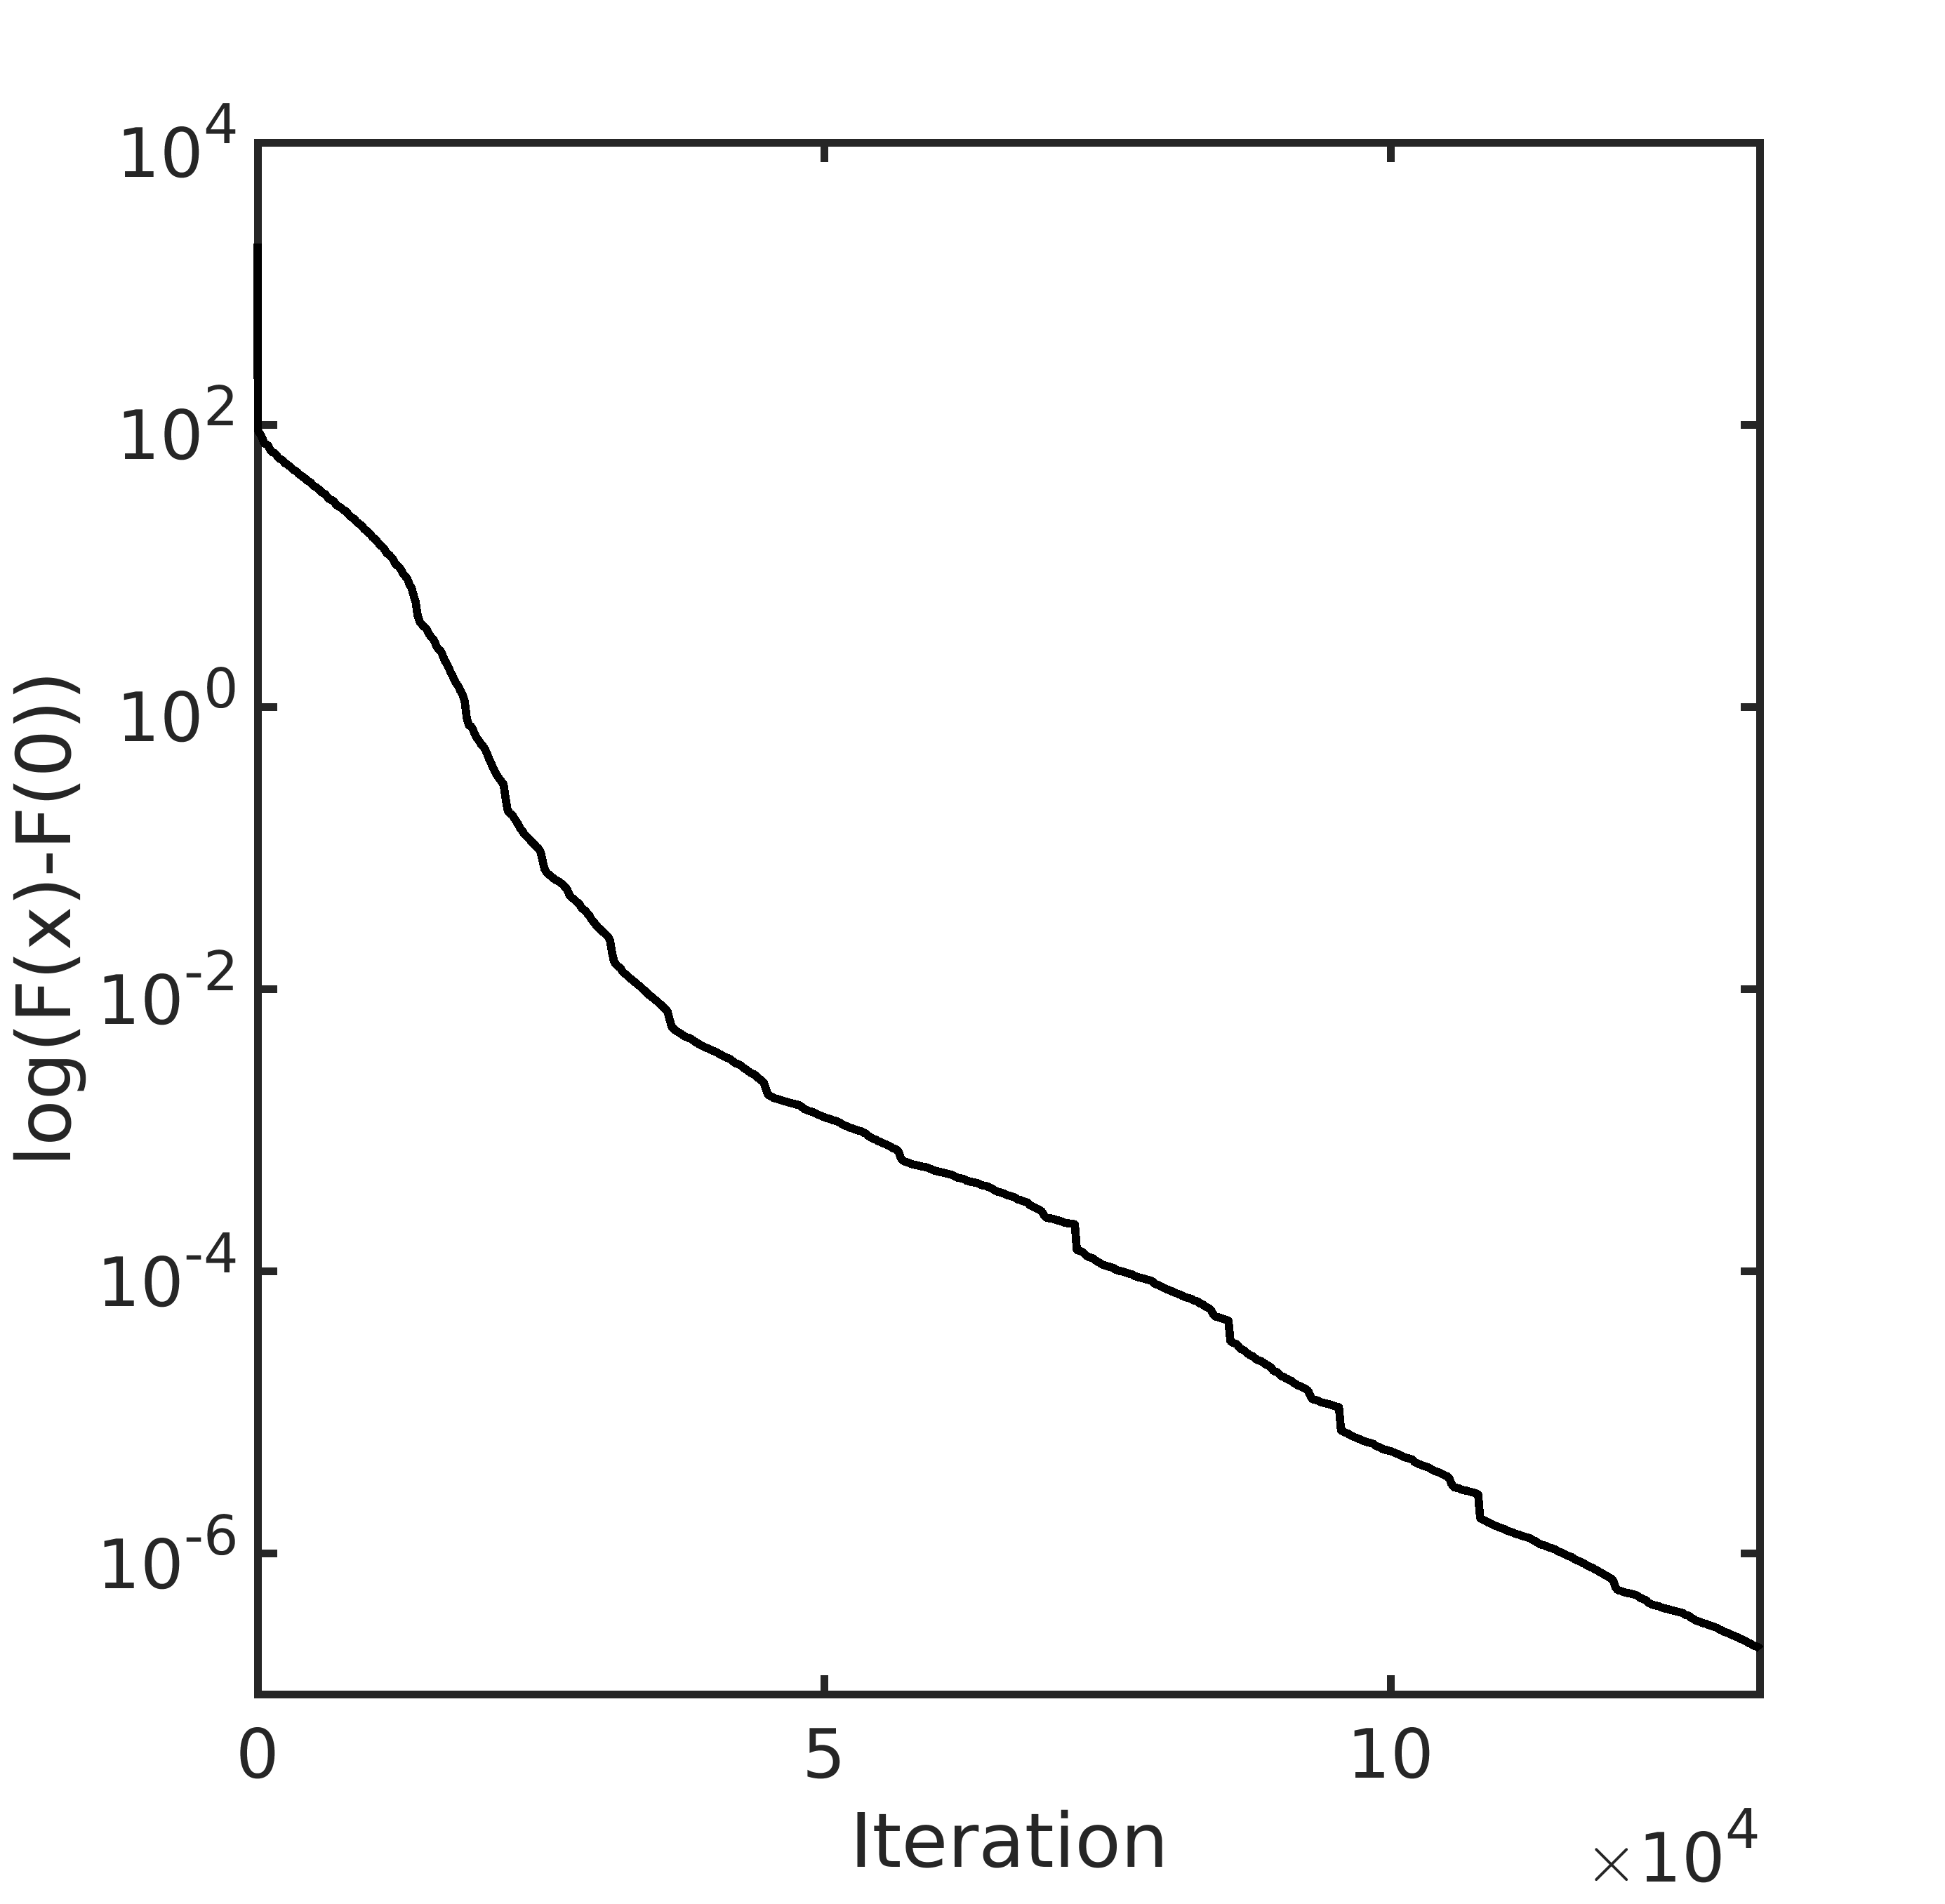
\includegraphics[scale=0.18]{./figures/arwhead640D.png}
	  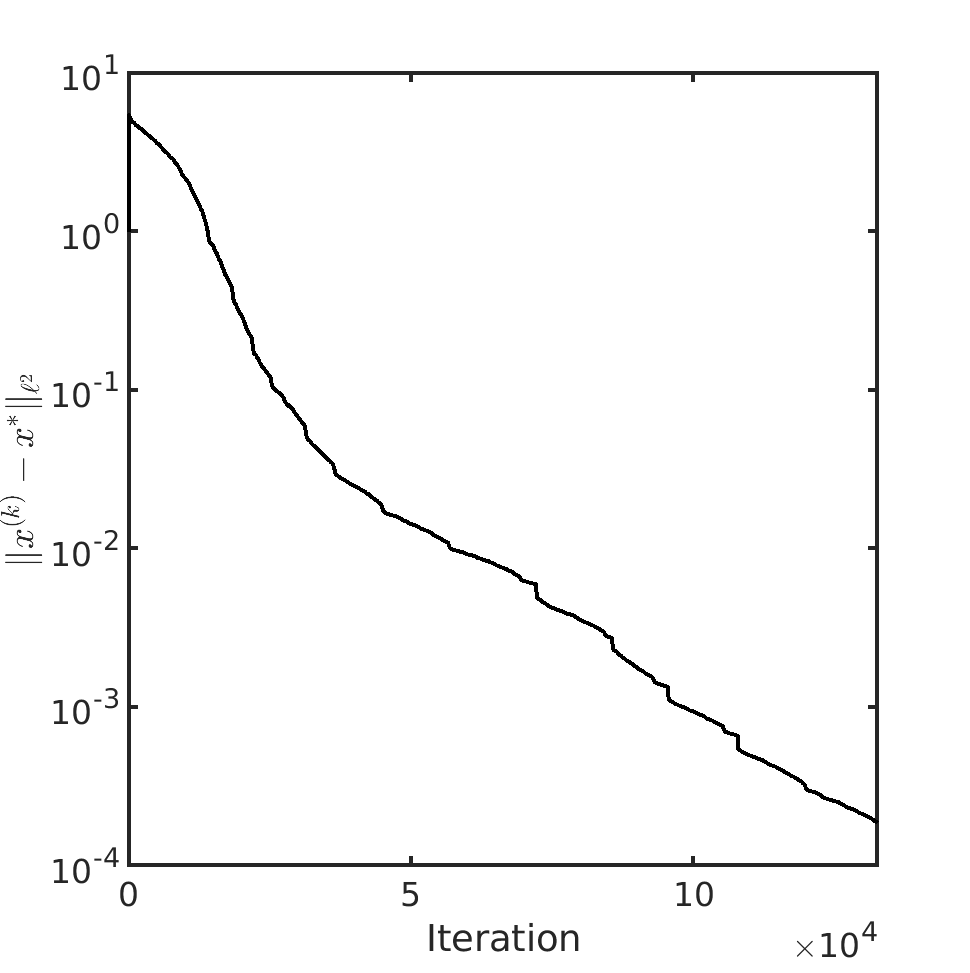
\includegraphics[scale=0.174]{./figures/arwhead640D_dist.png}
\end{figure}
\end{frame}
%%%%%%%%%%%%%%%%%%%%%%%%%%%%%%%%%%%%%%%%%%%%%%%%%%%%%%%%%%%%%%%%%%%%

%%%%%%%%%%%%%%%%%%%%%%%%%%%%%%%%%%%%%%%%%%%%%%%%%%%%%%%%%%%%%%%%%%%%%
%\begin{frame}{640D ARWHEAD Function: HiCSa}
%
%%\footnotesize{
%%%The global minimizer is $(1,1,\dots,1)$ with $f=0$.
%%%The initial value $x_j^{(0)}=-3.0$ if
%%%$j$ is even, and  $x_j^{(0)}=-1.0$ if $j$ odd.
%%%The choices of $n$ are $4$, $20$, $80$, $320$, $1280$, $2000$.
%%We can further apply HiCSa approach ($\eta=0.5$) to approximating the
%%minimizer of ARWHEAD function based on the above convergent results.
%%Here we take $n=640$ as an example to demonstrate the iteration procedure.
%%}
%
%\begin{figure}[!htbp]
%    \centering
%      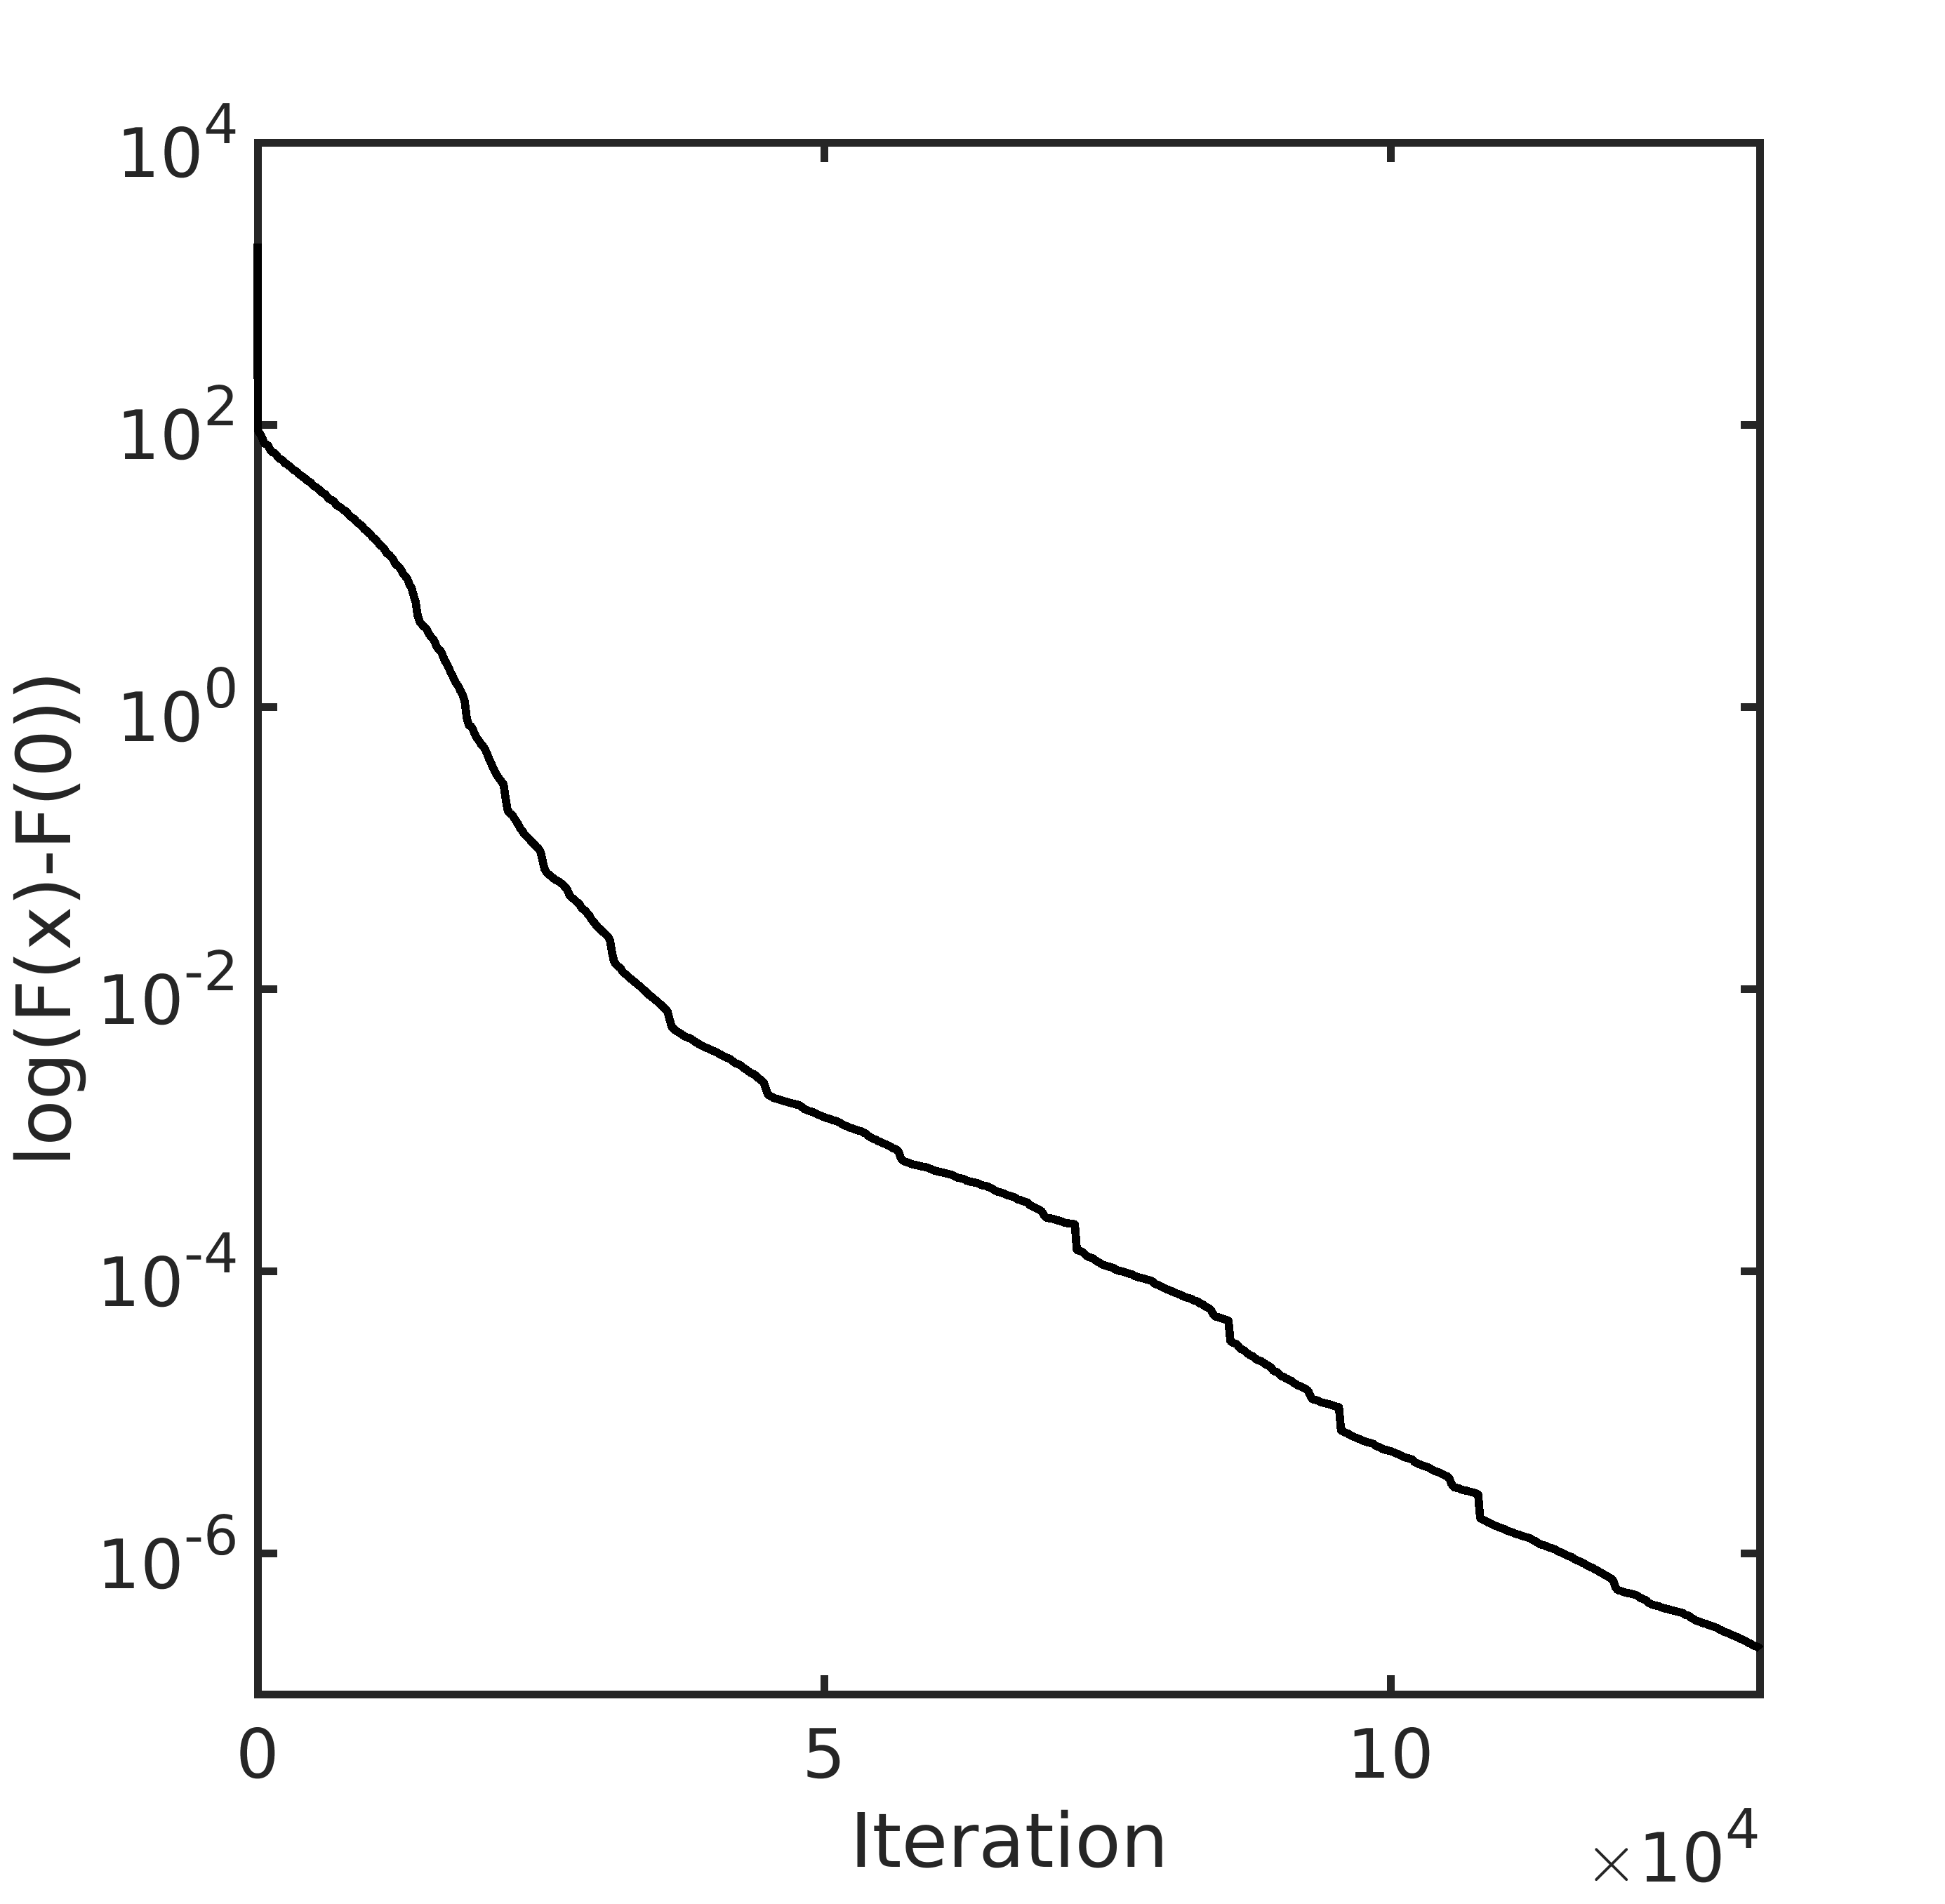
\includegraphics[scale=0.2]{./figures/arwhead640D.png}
%      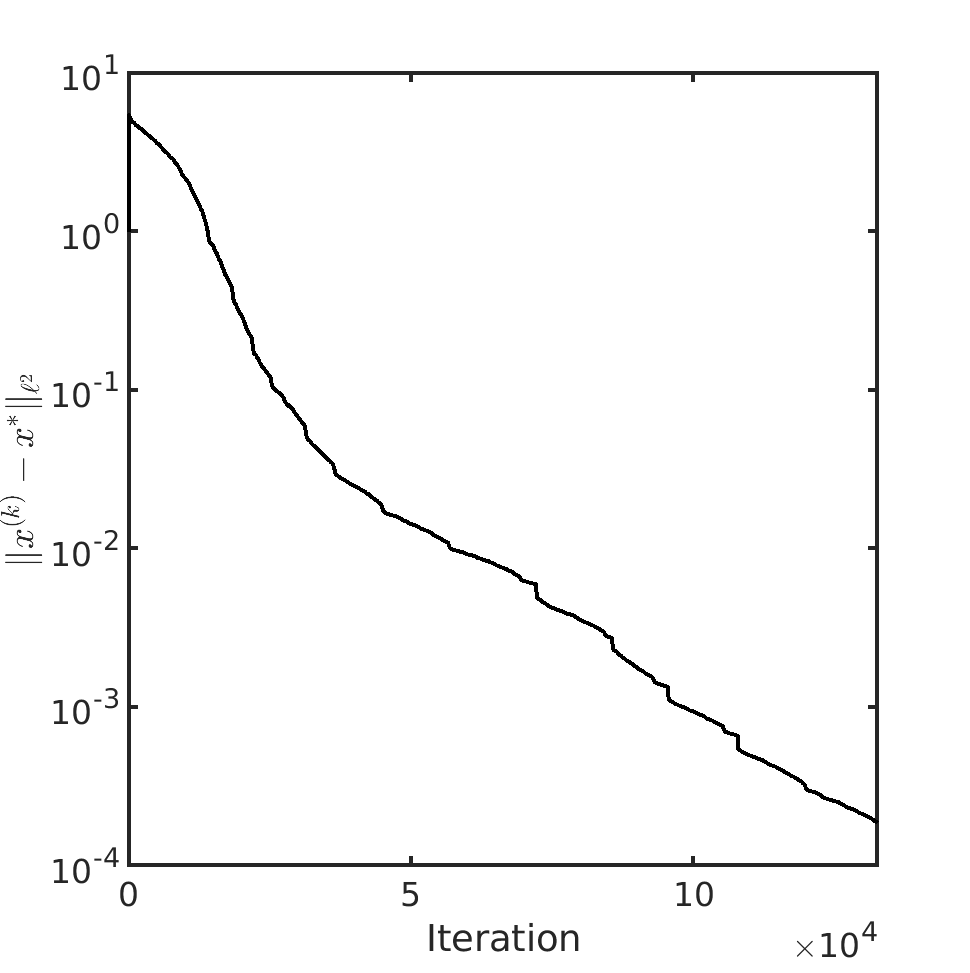
\includegraphics[scale=0.2]{./figures/arwhead640D_dist.png}
%\end{figure}
%%\begin{table}[!htbp]
%%\begin{center}
%%\begin{tabular}{|c|c|c|c|}
%% \hline
%%  $\rho$ &  Iter. & $\ell^2$-distance & $F(x)$
%% \\\hline
%%3.0 &  \makecell{ 8 } & 5.1575248543 & 9.4421477077e+01
%% \\\hline
%%1.5 &  \makecell{ 1 } & 5.1575248543e+00 & 9.4421477077e+01
%% \\\hline
%%0.75&  \makecell{ 8} & 5.3783368474e+00 & 9.3094586195e+01
%% \\\hline
%%0.375& \makecell{ 20} & 5.2806270221e+00 & 9.0804113723e+01
%% \\\hline
%%0.3125&  \makecell{ } & 1.8360260079e+01 & 1.5109701558e+02
%% \\\hline
%%0.15625&  \makecell{} &1.8016780347e+01 & 1.3743030983e+02
%% \\\hline
%%0.078125&  \makecell{ } & 1.6797229774e+01 & 1.1172829143e+02
%% \\\hline
%%0.0390625&  \makecell{ } & 3.4599901068e-01 & 5.9343258280e-01
%% \\\hline
%%1.953125e-02&  \makecell{ } & 2.6356847290e-01 & 2.1158089641e-01
%% \\\hline
%% $\downarrow$ & $\downarrow$ & $\downarrow$  & $\downarrow$
%% \\\hline
%%1.907349e-05 &   & 1.6760506513e-03 & 7.4452909429e-07
%% \\\hline
%%\end{tabular}
%%\\
%%\vspace{0.3cm}
%%It costs $102820247$ function evaluations.
%%\end{center}
%%\end{table}
%%\begin{itemize}
%%    \item It costs $102820247$ function evaluations.
%%\end{itemize}
%\end{frame}
%%%%%%%%%%%%%%%%%%%%%%%%%%%%%%%%%%%%%%%%%%%%%%%%%%%%%%%%%%%%%%%%%%%%%

\subsection{CHROSEN Function}
%%%%%%%%%%%%%%%%%%%%%%%%%%%%%%%%%%%%%%%%%%%%%%%%%%%%%%%%%%%%%%%%%%%%
\begin{frame}{CHROSEN Function}

\footnotesize{
\begin{align*}
	F(x) = \sum_{i=1}^{n-1}[(4(x_i-x_{i+1}^2)^2 + (1-x_{i+1})^2]
\end{align*}

The least value of $F$ is zero, which occurs when the variables take the values
$x_j=1$, $j=1,2,\dots,n$.
We apply HiCSa method ($\eta=0.5$) to 100D ARWHEAD function.
The starting vector is given by $x_j^{(0)}=-1$, $j=1,2,\dots,n$, as
Powell (2006) done. The search radius $\rho_0=5$ and $m_{\max}=32$.
}
%\begin{table}[!htbp]
%\begin{center}
%\begin{tabular}{|c|c|c|c|c|}
% \hline
%n & Iterations & $\ell^2$-distance & $F(x)$ & \# $F$
%\\ \hline
%10 & 4 & 6.5265183871 & 1.5837733615e+02 & 385
%\\ \hline
%20 & 4 & 9.0819518618 & 3.5637947273e+02 & 735
%\\ \hline
%40 & 4 & 1.2744786380e+01 & 7.5555050776e+02 & 1435
%\\ \hline
%80 & 4 & 1.7955627488e+01 & 1.5551760463e+03 & 2835
%\\ \hline
%\textcolor{blue}{100} & 4 & 2.0059901364e+01 & 1.9551042713e+03 & 3535
%%\\ \hline
%%160 & 4 & 2.5345459638e+01 & 3.1549985332e+03 & 5635
%%\\ \hline
%%320 & 4 & 3.5810421333e+01 & 6.3549121714e+03 & 11235
%%\\ \hline
%%640 & 4 & 5.0619988830e+01 & 1.2754869585e+04 & 22435
%%\\ \hline
%%1000 &  & & &
%\\ \hline
%\end{tabular}
%\end{center}
%\end{table}
%
\begin{figure}[!htbp]
	\centering
	  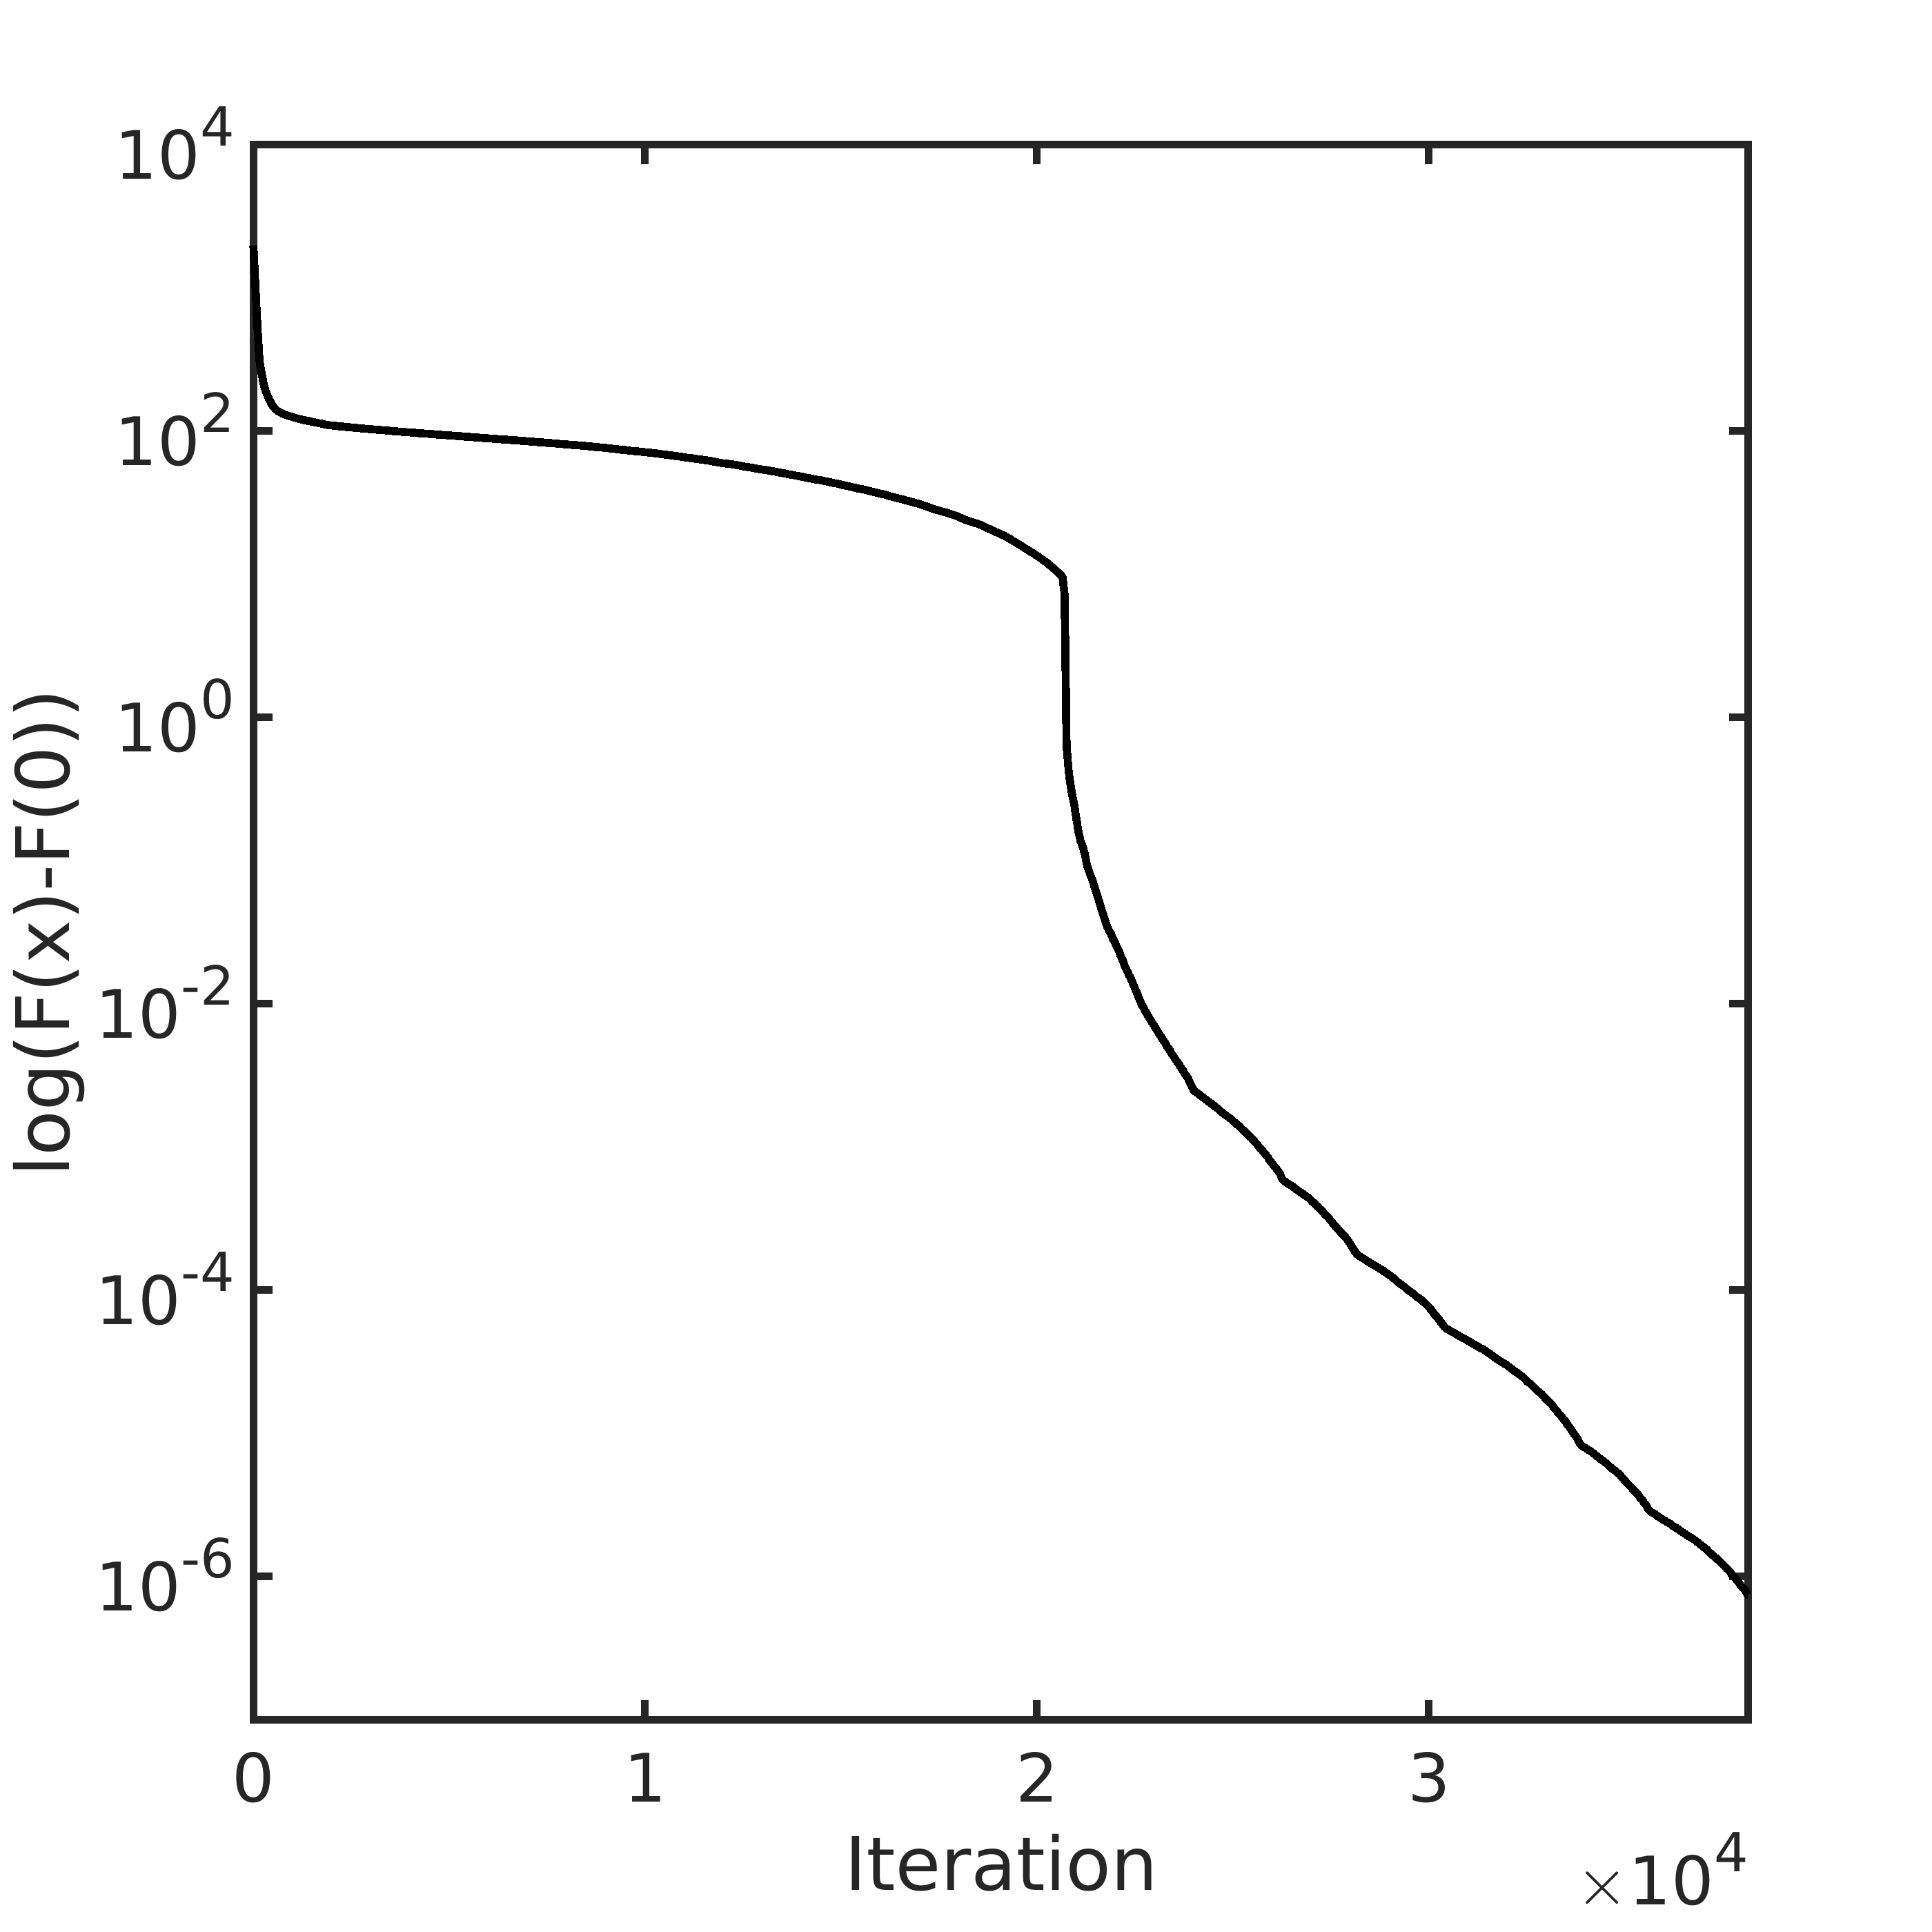
\includegraphics[scale=0.18]{./figures/chrosen100D.png}
	  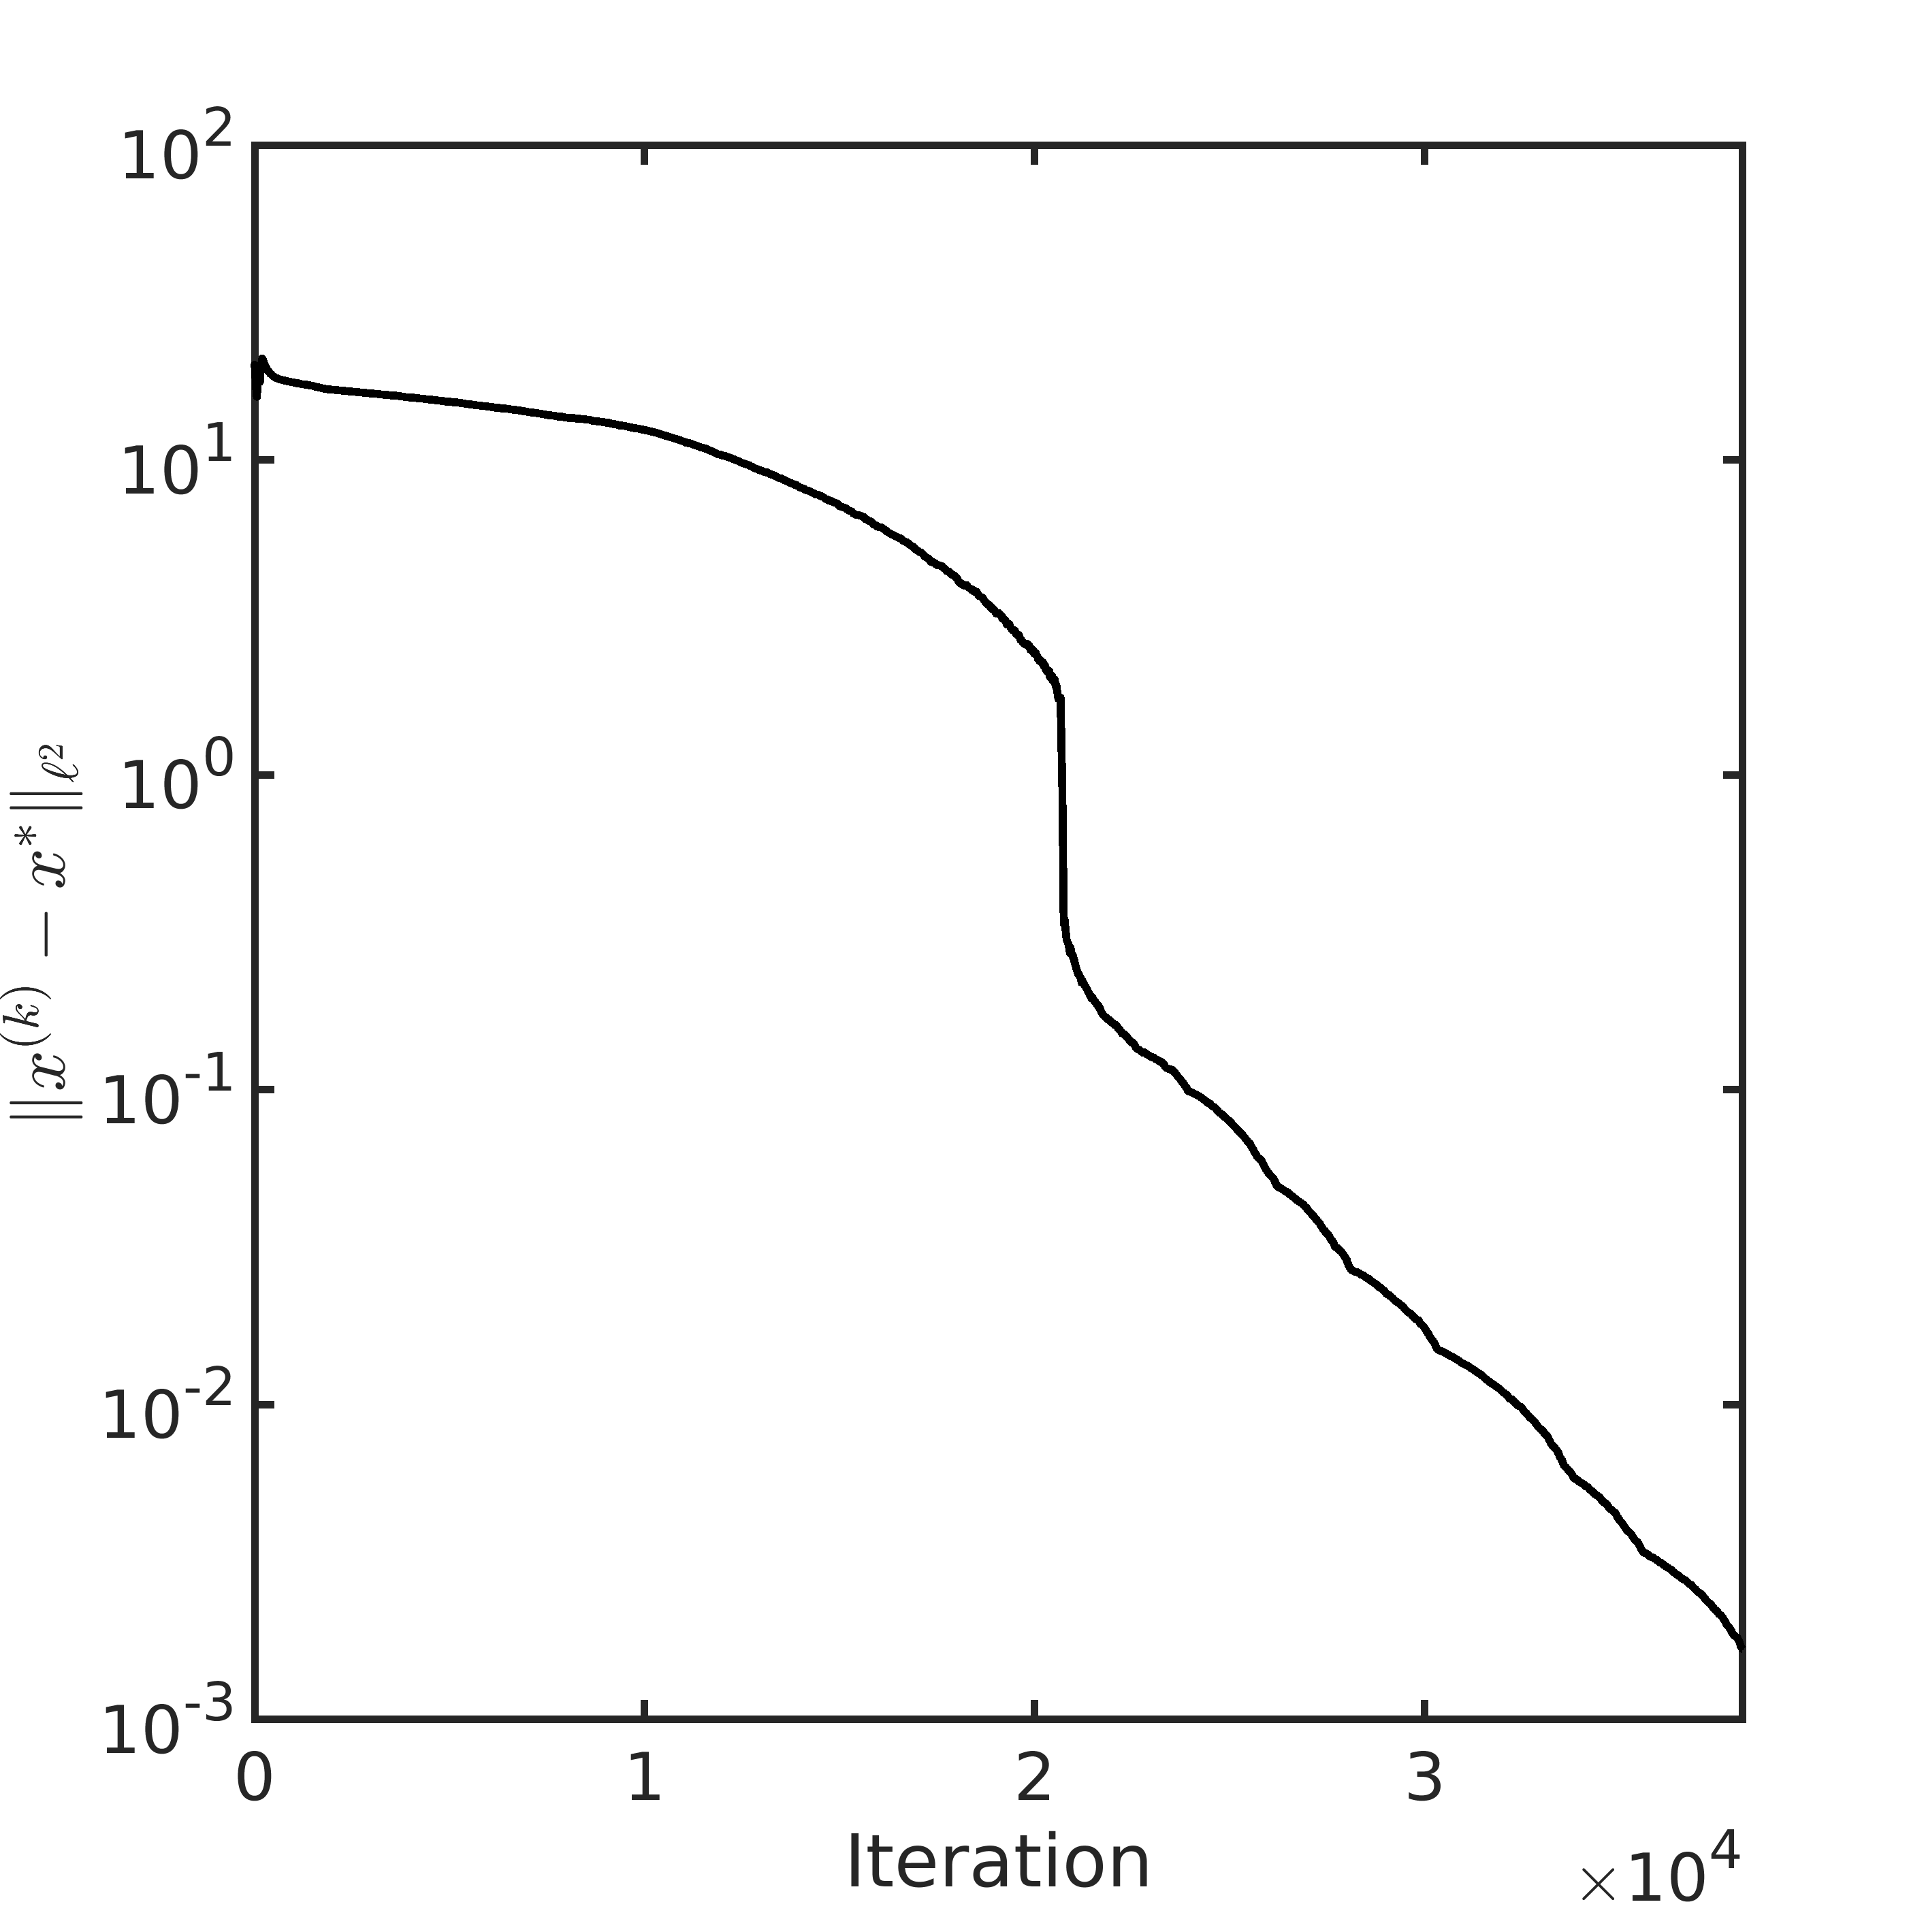
\includegraphics[scale=0.18]{./figures/chrosen100D_dist.png}
\end{figure}
\end{frame}
%%%%%%%%%%%%%%%%%%%%%%%%%%%%%%%%%%%%%%%%%%%%%%%%%%%%%%%%%%%%%%%%%%%%

%%%%%%%%%%%%%%%%%%%%%%%%%%%%%%%%%%%%%%%%%%%%%%%%%%%%%%%%%%%%%%%%%%%%%
%\begin{frame}{100D CHROSEN Function: HiCSa}
%
%\footnotesize{
%}
%%The global minimizer is $(1,1,\dots,1)$ with $f=0$.
%%The initial value $x_j^{(0)}=-3.0$ if
%%$j$ is even, and  $x_j^{(0)}=-1.0$ if $j$ odd.
%%The choices of $n$ are $4$, $20$, $80$, $320$, $1280$, $2000$.
%We can further apply HiCSa approach ($\eta=0.5$) to approximating the
%minimizer of CHROSEN function based on the above convergent results.
%Here we take $n=100$ as an example to demonstrate the iteration procedure.
%
%
%\begin{table}[!htbp]
%\begin{center}
%\begin{tabular}{|c|c|c|c|}
% \hline
%  $\rho$ &  Iter. & $\ell^2$-distance & $F(x)$
% \\\hline
%5.0 &  \makecell{ 4 } & 2.0059901364e+01 & 1.9551042713e+03
% \\\hline
%2.5 &  \makecell{ 100 } & 1.9298882974e+01 & 5.7446634570e+02
% \\\hline
%1.25&  \makecell{ 159 } & 1.9983269649e+01 & 2.1589406544e+02
% \\\hline
%0.625& \makecell{ 107 } & 1.8997693803e+01 & 1.7523312604e+02
% \\\hline
%0.3125&  \makecell{ 124 } & 1.8360260079e+01 & 1.5109701558e+02
% \\\hline
%0.15625&  \makecell{150 } &1.8016780347e+01 & 1.3743030983e+02
% \\\hline
%0.078125&  \makecell{1166 } & 1.6797229774e+01 & 1.1172829143e+02
% \\\hline
%0.0390625&  \makecell{18953 } & 3.4599901068e-01 & 5.9343258280e-01
% \\\hline
%1.953125e-02&  \makecell{232 } & 2.6356847290e-01 & 2.1158089641e-01
% \\\hline
% $\downarrow$ & $\downarrow$ & $\downarrow$  & $\downarrow$
% \\\hline
%1.907349e-05 & 2566  & 1.6760506513e-03 & 7.4452909429e-07
% \\\hline
%\end{tabular}
%\\
%\vspace{0.3cm}
%It costs $5217863$ function evaluations.
%\end{center}
%\end{table}
%
%\end{frame}
%%%%%%%%%%%%%%%%%%%%%%%%%%%%%%%%%%%%%%%%%%%%%%%%%%%%%%%%%%%%%%%%%%%%%
\section{Summary}
%%%%%%%%%%%%%%%%%%%%%%%%%%%%%%%%%%%%%%%%%%%%%%%%%%%%%%%%%%%%%%%%%%%%
\begin{frame}{Summary}
	\begin{itemize}
		\item Propose a
\textcolor{blue}{Hi}ll-\textcolor{blue}{C}limbing
	method with a \textcolor{blue}{S}tick (\textcolor{blue}{\textbf{HiCS}})
		\item Theory: \textcolor{blue}{Finite-step
			convergence} \textcolor{mypink3}{without convexity assumption}
		\item An efficient method of obtaining $O_h(x_k, \rho)$: \textcolor{blue}{Simplex	}
		\item Good properties:
			\begin{itemize}
				\item Only one parameter $\rho$ which can be adjusted
%                    (\textcolor{blue}{2500D Ackley function})
%                \item Be able to capture the local and global optimal states
				\item Capture the neighborhood of a minimizer
				\item Has potential to approximate the global minimizer
				\item Be able to implement to high dimension
			\end{itemize}
	\end{itemize}
\end{frame}
%%%%%%%%%%%%%%%%%%%%%%%%%%%%%%%%%%%%%%%%%%%%%%%%%%%%%%%%%%%%%%%%%%%%

%%%%%%%%%%%%%%%%%%%%%%%%%%%%%%%%%%%%%%%%%%%%%%%%%%%%%%%%%%%%%%%%%%%%
\begin{frame}
	\begin{centering}
	  \Huge Thanks for Your Attention ! \par
	\end{centering}
\end{frame}
%%%%%%%%%%%%%%%%%%%%%%%%%%%%%%%%%%%%%%%%%%%%%%%%%%%%%%%%%%%%%%%%%%%%

%%%%%%%%%%%%%%%%%%%%%%%%%%%%%%%%%%%%%%%%%%%%%%%%%%%%%%%%%%%%%%%%%%%%%
%\newcount\opaqueness
%\plainframe{
%  \itshape
%  \animate<1-10>
%  \Large
%
%  \only<1-10>{
%  \animatevalue<1-10>{\opaqueness}{10}{100}
%  \begin{colormixin}{\the\opaqueness!averagebackgroundcolor}
%    \begin{centering}
%      \Huge Thanks for Your Attention \par
%    \end{centering}
%  \end{colormixin}
%  }
%}
%%%%%%%%%%%%%%%%%%%%%%%%%%%%%%%%%%%%%%%%%%%%%%%%%%%%%%%%%%%%%%%%%%%%%


%\section{Some \LaTeX{} Examples}
%
%\subsection{Tables and Figures}
%
%\begin{frame}{Tables and Figures}
%
%\begin{itemize}
%\item Use \texttt{tabular} for basic tables --- see Table~\ref{tab:widgets}, for example.
%\item You can upload a figure (JPEG, PNG or PDF) using the files menu.
%\item To include it in your document, use the \texttt{includegraphics} command (see the comment below in the source code).
%\end{itemize}
%
%% Commands to include a figure:
%%\begin{figure}
%%\includegraphics[width=\textwidth]{your-figure's-file-name}
%%\caption{\label{fig:your-figure}Caption goes here.}
%%\end{figure}
%
%\begin{table}
%\centering
%\begin{tabular}{l|r}
%Item & Quantity \\\hline
%Widgets & 42 \\
%Gadgets & 13
%\end{tabular}
%\caption{\label{tab:widgets}An example table.}
%\end{table}
%
%\end{frame}
%
%\subsection{Mathematics}
%
%\begin{frame}{Readable Mathematics}
%
%Let $X_1, X_2, \ldots, X_n$ be a sequence of independent and identically distributed random variables with $\text{E}[X_i] = \mu$ and $\text{Var}[X_i] = \sigma^2 < \infty$, and let
%$$S_n = \frac{X_1 + X_2 + \cdots + X_n}{n}
%      = \frac{1}{n}\sum_{i}^{n} X_i$$
%denote their mean. Then as $n$ approaches infinity, the random variables $\sqrt{n}(S_n - \mu)$ converge in distribution to a normal $\mathcal{N}(0, \sigma^2)$.
%
%\end{frame}
%

\end{document}
